% Формат документа и размер шрифта
\documentclass[a4paper,12pt]{article}
\usepackage{lectures}
\begin{document}

\begin{titlepage}
  \begin{center}
  
  	{\HugeАлгоритмы и Структуры Данных}
	\\ \
	\\ \
	\\ \
	{\Huge \textbf{Мини-Кормен}}
    \\ \
    \\ \
    
    \begin{figure}[h]
    \begin{center}
        \begin{minipage}[h]{0.8\linewidth}
        \includegraphics[height=18cm, width=\linewidth]{mini-kormen.jpg}
        \end{minipage}
    \end{center}
    \end{figure}
    \ \\
    
    {\Large Вадим Гринберг} \\ 
    \ \\ 
    {\Large Алексей Хачиянц} \\ 
   
\end{center}
\end{titlepage}

\tableofcontents

\newpage

\section{Рекурсивные алгоритмы: задача о Ханойской башне. Оценка времени работы 
рекурсивного алгоритма при помощи рекуррентного соотношения. Доказательство 
оптимальности рекурсивного алгоритма.}

\subsection{Ханойские башни}
Рассмотрим классическую задачу, предложенную Эдуардом Люка в 1883 году. Есть 
три стержня, при этом на первый стержень нанизано 8 дисков. Нужно перенести все 
диски на другой стержень, соблюдая два правила: диски можно двигать только по 
одному и нельзя класть
диск большего радиуса на диск меньшего радиуса. Возможно ли это?

Придуманная профессором Люка легенда гласит, что в Великом храме города Бенарес,
 под собором, отмечающим середину мира, находится бронзовый диск, на котором 
 укреплены 3 алмазных стержня, высотой в один локоть и толщиной с пчелу. 
 Давным-давно, в самом начале времён, монахи этого монастыря провинились перед 
 богом Брахмой. Разгневанный Брахма воздвиг три высоких стержня и на один из 
 них возложил 64 диска, сделанных из чистого золота. Причем так, что каждый 
 меньший диск лежит на большем.

Как только все 64 диска будут переложены со стержня, на который Брахма сложил 
их при создании мира, на другой стержень, башня вместе с храмом обратятся в пыль
 и под громовые раскаты погибнет мир.

Интуиция подсказывает, что это возможно. Но каков тогда алгоритм и сколько 
операций ему необходимо?

Чтобы переместить $n$ дисков с первого стержня на второй, можно сначала 
переместить $n - 1$ диск на третий стержень, перенести самый большой диск на 
второй стержень, а затем переместить $n - 1$ диск с третьего стержня на второй. 
Такое рекурсивное решение представлено в Алгоритме \ref{algo:hanoi}.

\begin{algorithm}[H]
	\caption{Рекурсивный алгоритм решения задачи о Ханойской башне}
	\label{algo:hanoi}
	\begin{algorithmic}[1]
		\Require Число дисков $n$, начальный $i$, конечный $j$ и вспомогательный 
		$k$ стержни.
		\Ensure Последовательность пар $(x, y)$, соответствующих перемещению диска 
		со стержня $x$ на стержень $y$, приводящая к перемещению $n$ верхних дисков 
		со стержня $i$ на стержень $j$.
		\Function{Hanoi3}{$n,i,j,k$}
			\If{$n > 0$}
				\State \textsc{Hanoi3}($n-1,i,j,k$)
				\State move $i \to k$
				\State \textsc{Hanoi3}($n-1,k,j,i$)
			\EndIf
		\EndFunction
	\end{algorithmic}
\end{algorithm}

Покажем с помощью дерева операций, как алгоритм работает для трёх дисков:

\begin{center}
	\begin{forest}
		for tree={
			parent anchor=south,
			child anchor=north,
			if n children=0{
				font=\itshape,
				tier=terminal,
			}{},
		}
		[{H(3,1,2,3)} [{H(2,1,3,2)} [{H(1,1,2,3)} [$1 \to 2$]]
		[$1 \to 3$]
		[{H(1,2,3,1)} [$2 \to 3$]]]
		[$1 \to 2$] 
		[{H(2,3,2,1)} [{H(1,3,1,2)} [$3 \to 1$]]
		[$3 \to 2$]
		[{H(1,1,2,3)} [$1 \to 2$]]]]
	\end{forest}
\end{center}

По сути, данный алгоритм обходит дерево в глубину, выполняя необходимые 
перестановки.

\subsection{Оптимальность рекурсивного алгоритма и время его работы.}

Докажем, что данный алгоритм является \textbf{оптимальным}, то есть нет 
алгоритма, который бы решал эту же задачу быстрее.

Пусть $T_n$~--- минимальное количество операций, за которое можно перенести 
$n$ дисков. Сразу же заметим, что для переноса 0 дисков действий вообще не 
нужно. Тогда $T_0 = 0$.

Показанный ранее алгоритм показывает, что 
$T_n \leqslant 2T_{n - 1} + 1\text{ для } n > 0.$

Возникает логичный вопрос: а можно ли быстрее? Увы, но нет. Рано или поздно 
придётся перенести самый широкий диск. Но для этого необходимо поставить 
$n - 1$ диск на один стержень. Тогда можно сделать вывод, что $T_n \geqslant 
2T_{n - 1} + 1\text{ для } n > 0.$

Отсюда получаем, что минимальное количество операций задаётся следующим 
\emph{рекуррентным соотношением}:

\[T_n = \begin{cases}
2T_{n - 1} + 1, & n > 0 \\
0, & n = 0
\end{cases}\]

Прекрасно. Мы знаем, что алгоритм \ref{algo:hanoi} наиболее оптимален и знаем 
рекуррентное соотношение, задающее количество операций. Но можно ли найти 
\emph{замкнутую} формулу~--- такую, что она сразу даст нужное значение? Да, 
можно.

\begin{theorem}
	$T_n = 2^{n} - 1$
\end{theorem}
\begin{proof}
	Докажем это по индукции. База верна, так как $T_0 = 0 = 2^{0} - 1$. Теперь 
	пусть предположение верно для $n - 1$, то есть $T_{n - 1} = 2^{n - 1} - 1$.
	 Тогда \[T_{n} = 2T_{n - 1} + 1 = 2(2^{n - 1} - 1) + 1 = 2^n - 2 + 1 = 2^n - 1\qedhere\]
\end{proof}

Теперь немного изменим задачу.
\subsection{Четыре стержня}

Допустим, что у нас четыре стержня, два из которых --- вспомогательные. Обозначим
\[n_m = \sum_{i=1}^mi = \frac{m(m+1)}{2}.\]
Для простоты предположим, что изначально на первом стержне находится $n_m$ дисков.

Чтобы переместить $n_m$ дисков с первого стержня на второй, можно сначала 
переместить $n_{m-1}$ дисков на четвертый стержень, затем переместить оставшиеся
 $m$ самых больших дисков на второй стержень, используя Алгоритм \ref{algo:hanoi}
  и третий стержень в качестве вспомогательного, и наконец переместить $n_{m-1}$
   дисков с четвертого стержня на второй. Такое рекурсивное решение представлено
    в Алгоритме \ref{algo:hanoi4}.

\begin{algorithm}[H]
	\caption{Рекурсивный алгоритм решения задачи о Ханойской башне на 4-х стержнях}
	\label{algo:hanoi4}
	\begin{algorithmic}[1]
		\Require Число дисков $n_m = m(m+1)/2$, начальный $i$, конечный $j$ и 
		вспомогательные $k$ и $l$ стержни.
		\Ensure Последовательность пар $(x, y)$, соответствующих перемещению диска 
		со стержня $x$ на стержень $y$, приводящая к перемещению $n$ верхних дисков
		 со стержня $i$ на стержень $j$.
		\Function{Hanoi4}{$n_m,i,j,k,l$}
			\If{$n > 0$}
				\State \textsc{Hanoi4}($n-m,i,l,k,j$)
				\State \textsc{Hanoi3}($m,i,j,k$)
				\State \textsc{Hanoi4}($n-m,l,j,i,k$)
			\EndIf
		\EndFunction
	\end{algorithmic}
\end{algorithm}

Алгоритм \ref{algo:hanoi4} можно обобщить на случай произвольного числа дисков 
$n$, например, так: на верхнем уровне рекурсии выбрать $n_{m-1}$, ближайшее 
снизу к $n$, а вместо $m$ в вызове алгоритма \algname{Hanoi3} использовать 
$n - n_m$.

Обозначим за $g(n_m)$ число шагов, требующихся Алгоритму \ref{algo:hanoi4} для 
решения задачи с $n_m$ дисками. Получаем следующее рекуррентное соотношение:
\[g(n_m) = \begin{cases}
	0, & n_m = 0; \\
	2g(n_{m-1}) + 2^m - 1, & n > 0.
	\end{cases}\]

Докажем по индукции, что $g(n_m) = (m - 1)2^m + 1$ (эту оценку можно получить, проанализировав дерево рекурсии).
\begin{description}
	\item[Базис:] $g(n_0) = 0 = -1 + 1 = (0 - 1) \cdot 2^0 + 1$.
	\item[Шаг:] Предположим, что $g(n_{m-1}) = (m - 2)2^{m-1} + 1$. Тогда
	\begin{align*} % requires amsmath; align* for no eq. number
	   g(n_m) = {}& 2g(n_{m-1}) + 2^m - 1 = \\
	   = {}& 2((m - 2)2^{m-1} + 1) + 2^m - 1 = \\
	   = {}& (m - 2)2^m + 2 + 2^m - 1 = \\
	   = {}& (m - 1)2^m + 1.
	\end{align*}
\end{description}

Таким образом, число шагов асимптотически зависит от числа входных дисков $n$ как $\Theta(\sqrt{n}2^{\sqrt{2n}})$.\footnote{Смысл этого утверждения уточним на следующих лекциях.} Можно ли переместить диски быстрее --- открытый вопрос.

Как можно обобщить Алгоритм \ref{algo:hanoi4} на случай произвольного числа стержней? Сработает ли такой вариант?

\begin{algorithm}[H]
	\caption{Рекурсивный алгоритм решения задачи о Ханойской башне, общий случай}
	\label{algo:hanoik}
	\begin{algorithmic}[1]
		\Require Число дисков $n_m = m(m+1)/2$, начальный $i$, конечный $j$ и множество вспомогательных $P$ стержней.
		\Ensure Последовательность пар $(x, y)$, соответствующих перемещению диска со стержня $x$ на стержень $y$, приводящая к перемещению $n$ верхних дисков со стержня $i$ на стержень $j$.
		\Function{Hanoi}{$n,i,j,P$}
			\If{$n > 0$}
				\State choose $p \in P$
				\State $R \mathrel{:=} P \setminus p$
				\If{$R = \varnothing$}
					\State \textsc{Hanoi3}($n,i,j,p$)
				\Else
					\State \textsc{Hanoi}($n-m,i,p,R \cup \{j\}$)
					\State \textsc{Hanoi}($m,i,j,R$)
					\State \textsc{Hanoi}($n-m,p,j,R \cup \{i\}$)
				\EndIf
			\EndIf
		\EndFunction
	\end{algorithmic}
\end{algorithm}
\newpage
\section{$O$-, $o$-, $\Omega$-, $\omega$-, $\Theta$- обозначения. Оценка сложности алгоритмов.}

\subsection{Асимптотические обозначения}

Введем следующие обозначения:

\[\Theta(g(n)) = \left\{ f(n)\mid \exists c_1>0, c_2>0 \exists n_0: \forall n \geqslant n_0 \implies 0\leqslant c_1g(n)\leqslant f(n) \leqslant c_2g(n) \right\},\]

$\Theta$ --- \emph{асимптотическое} $=$. Например, $2n = \Theta(n)$. По определению, $c_1n \leqslant 2n \leqslant c_2n$. Тогда $c_1 = 1, c_2 = 2$.

\[O(g(n)) = \left\{ f(n)\mid \exists  c_2>0 \exists n_0: \forall n \geqslant n_0 \implies 0\leqslant f(n) \leqslant c_2g(n) \right\}\]

$O$ --- \emph{асимптотическое} $\leqslant$. Например, по этому определению $n = O(n \log{n})$, так как при достаточно больших $n_0$ $\log n_0 > 1$. Тогда $c_2 = 1$.

\[\Omega(g(n)) = \left\{ f(n)\mid \exists c_1>0 \exists n_0: \forall n \geqslant n_0 \implies 0\leqslant c_1g(n)\leqslant f(n) \right\}\]

$\Omega$ --- \emph{асимптотическое} $\geqslant$. Например, $n \log n = \Omega(n \log n)$ и $n \log n = \Omega(n)$. В обоих случаях подходит $c_1 = 1$.

\[o(g(n)) = \left\{ f(n)\mid \forall  c_2>0 \exists n_0: \forall n \geqslant n_0 \implies 0\leqslant f(n) \leqslant c_2g(n) \right\}\]

$o$ --- \emph{асимптотическое} $<$. Например, $n = o(n \log n)$. Покажем это. Пусть $n < c_2 n \log n \iff 1 < c_2 \log n \iff n > 2^{1/c_2}$. Тогда $n_0 = [2^{1/c_2} + 1]$

\[\omega(g(n)) = \left\{ f(n)\mid \forall c_1>0 \exists n_0: \forall n \geqslant n_0 \implies 0\leqslant c_1g(n)\leqslant f(n) \right\}\]

$\omega$ --- \emph{асимптотическое} $>$. Например, нельзя сказать, что $n \log n = \omega(n \log n)$. Но можно сказать, что  $n \log n = \omega(n)$.

Когда мы пишем такую нотацию, мы подразумеваем функции, а не числа. Если же указывать функции явно, то это можно сделать с помощью $\lambda$-нотации:

\[\lambda n.n \in o(\lambda n.n \log_2 n)\]

\textbf{Примечание:} данная нотация очень похожа на лямбда-функции в Python:
\[\verb|lambda x: x * x| \iff \lambda x. x^2\] 

Заметим, что в логарифмах можно свободно менять основание: $\log_c n = \frac {\log_2 n}{\log_2 c}$. Именно поэтому не пишут основание логарифма.
\newpage
\section{Сортировка вставкой и слиянием. Использование инварианта цикла при доказательстве корректности сортировки вставкой}

\subsection{Задача сортировки}
Одна из классических задач мира алгоритмов, встречающаяся на практике повсеместно~--- \emph{задача сортировки}. Поставим её формально.

\textbf{Вход:} последовательность из $n$ чисел $[a_{1}, a_{2}, \ldots, a_{n}]$.

\textbf{Выход:} последовательность из $n$ чисел $[a'_{1}, a'_{2}, \ldots, a'_{n}]$ такая, что $a'_{1} \leqslant a'_{2} \leqslant \ldots \leqslant a'_{n}$.

Вообще говоря, на вход может подаваться последовательность, состоящая из элементов любого линейно упорядоченного множества.

\subsection{Сортировка вставкой} 
Рассмотрим алгоритм \emph{сортировки вставками}:

\begin{algorithm}[H]
	\caption{Алгоритм сортировки вставками}
	\label{algo:insertion-sort}
	\begin{algorithmic}[1]
		\Require Массив $a[1..n]$ из $n$ чисел. 
		\Ensure Массив $a$ становится отсортированным по возрастанию.
		\Function{Insertion-Sort}{$A$}
		\For{$j \mathrel{:=} 2$ \textbf{to} $A.length$}\Comment{вставка $A[j]$ в отсортированный массив $A[1..j - 1]$}
		\State $key \mathrel{:=} A[j]$
		\State $i \mathrel{:=} j - 1$
		\While{$i > 0$ \textbf{and} $A[i] > key$}
		\State $A[i + 1] \mathrel{:=} A[i]$
		\State $i \mathrel{:=} i - 1$
		\EndWhile
		\State $A[i + 1] \mathrel{:=} key$
		\EndFor
		\EndFunction
	\end{algorithmic}
\end{algorithm}

По сути, мы поочередно добавляем каждый $i + 1$-ый элемент в отсортированную подпоследовательность из первых $i$ элементов так, чтобы последовательность оставалась отсортированной.

\subsection{Корректность алгоритма сортировки вставками.}
Возникает логичный вопрос~--- а можем ли мы сказать, что этот алгоритм делает именно то, что нам нужно? Другими словами, \emph{корректен} ли он? Оказывается, что да. Докажем это.

Для этого стоит рассмотреть так называемый \emph{инвариант цикла}~--- нечто, что не изменяется при переходе на следующую итерацию цикла. В данном случае он будет таков: на $j$-й итерации цикла первые $i - 1$ элементов массива будут упорядочены.

Далее нужно рассмотреть три свойства инварианта цикла:
\begin{itemize}
	\item \textbf{Инициализация:} Инвариант цикла выполняется на первой итерации;
	
	\item \textbf{Переход:} Инвариант сохраняется при переходе на следующую итерацию;
	
	\item \textbf{Завершение:} При окончании цикла инвариант даёт какое-то ценное свойство полученного массива.
	\end{itemize}
	Можно сказать, что первые два свойства доказывают корректность инварианта. Приступим:
	\begin{itemize}
		\item \textbf{Инициализация:} На первой итерации цикла элемент вставляется в массив из одного элемента. Но он, очевидно, отсортирован. Тогда инвариант цикла выполняется для первой итерации.
		
		\item \textbf{Переход:} Пусть массив $[a_1, \ldots, a_{j - 1}]$ уже отсортирован. В теле цикла делается следующее: до тех пор, пока $a_{j}$ меньше стоящего перед ним элемента, они меняются местами. По сути, элемент просто вставляется на нужное место. Тогда инвариант выполняется при переходе на следующую итерацию. Следовательно, инвариант корректен.
		
		\item \textbf{Завершение:} Цикл завершается тогда, когда $j = n + 1$. Заметим, что это будет итерация под номером $n$. Но тогда (согласно инварианту цикла) первые $n$ элементов массива, то есть весь массив, будут упорядочены. Тогда в конце массив окажется отсортированным. Тем самым мы доказали, что алгоритм корректен.
		\end{itemize}

\subsection{Время работы сортировки вставками.}
Хорошо, он корректен. Но насколько быстро он работает? Достаточно очевидны три факта:
\begin{itemize}
	\item Скорость работы зависит от входных данных;
	\item Чем больше элементов, тем дольше будет работать алгоритм;
	\item Если алгоритм уже отсортирован, то он будет работать быстрее.
	\end{itemize}
	Обычно время работы рассматривают в трёх случаях~--- в худшем, в лучшем и в среднем. Хотя оценка в лучшем случае не несёт особо ценной информации, так как всегда можно модифицировать алгоритм так, что на некоторых наборах данных он будет работать очень быстро.
	
	Для оценки времени работы введём асимптотическую оценку $\Theta$:
	\[\Theta(g(n)) = \{f(n)\mid\exists\,c_1, c_2 > 0: \forall n\geqslant n_0 \implies 0 \leqslant c_1g(n) \leqslant f(n) \leqslant c_2g(n)\}\]
	
	Рассмотрим следующий пример. Пусть $f(n) = 3n^2 + 2n + 6$. Тогда $f(n) \in \Theta(n^2)$. Хотя правильней писать так, но на практике все пишут, что $f(n) = \Theta(n^2)$.
	
	Стоит обратить внимание, что асимтотическая оценка показывает рост функции. Но не стоит забывать про константы~--- может выйти так, что для достаточно маленьких $n$ функция из $\Theta(n^3)$ работает быстрее, чем функция из $\Theta(n)$:
	\begin{center}
		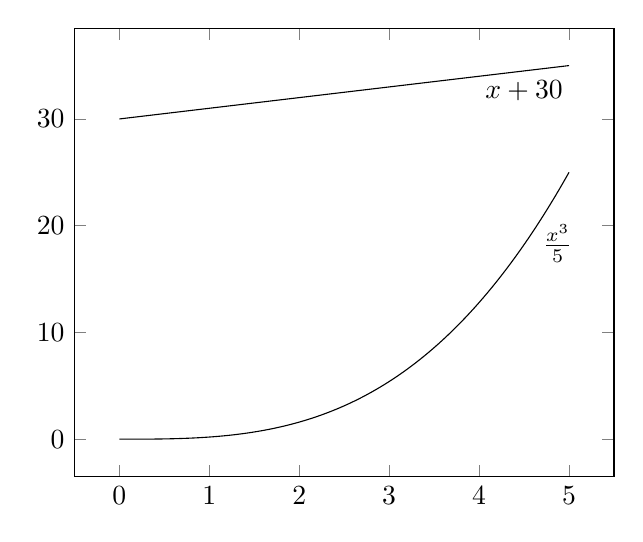
\begin{tikzpicture}
		\begin{axis}
		\addplot [domain=0:5, samples=101,unbounded coords=jump]{x+30} node[below,pos=0.9] {$x + 30$};
		\addplot [domain=0:5, samples=101,unbounded coords=jump]{0.2 * x^3} node[below,pos=0.85] {$\quad \frac{x^3}{5}$};
		\end{axis}
		\end{tikzpicture}
		\end{center}
		
		Вернёмся к оценке времени работы алгоритма. Пусть его скорость работы равна $T(n)$.
		
		Рассмотрим худший случай. Когда он достигается? Когда приходится делать максимальное число перестановок. Тогда на $i$-й итерации совершается $\Theta(i)$ операций. Следовательно, \[T(n) = \sum_{k = 0}^{n} \Theta(k) = \Theta(n^2).\]
		
		В среднем случае все исходы равновероятны. Тогда в среднем будет выполняться половина всех возможных перестановок. А это $\Theta(n^2)$.
		
		В лучшем случае не совершается ни одной перестановки. Это означает, что массив уже отсортирован. Тогда алгоритм работает за $\Theta(n)$ (так как он просто проходится по массиву).
		
\subsection{Сортировка слиянием}
Рассмотрим другой алгоритм --- \emph{сортировку слиянием}.

\begin{algorithm}[H]
	\caption{Алгоритм сортировки слиянием}
	\label{algo:merge-sort}
	\begin{algorithmic}[1]
		\Require Массив $a[1..n]$ из $n$ чисел. 
		\Ensure Отсортированный по возрастанию массив, содержащий в точности все элементы входного массива $a$.
		\Function{Merge-Sort}{$A$}
		\State $n \mathrel{:=} A.$length
		\If{$n > 1$}
		\State $B_1 \mathrel{:=} \textsc{Merge-Sort}\left(A\left[1: \lfloor n/2 \rfloor\right]\right)$
		\State $B_2 \mathrel{:=} \textsc{Merge-Sort}\left(A\left[\lfloor n/2 \rfloor + 1 : n\right]\right)$
		\State $A \mathrel{:=} \textsc{Merge}(B_1, B_2)$ \Comment{сливаем два отсортированных массива в один}
		\EndIf
		\State return $A$
		\EndFunction
	\end{algorithmic}
\end{algorithm}

В Алгоритме \ref{algo:merge-sort} мы делим массив на две (почти) равные части и сортируем каждую из них рекурсивно.
Функция \algname{Merge}, описанная в алгоритме \ref{algo:merge}, за линейное время <<сливает>> два отсортированных подмассива в один большой отсортированный массив. В качестве упражнения докажите корректность \algname{Merge}. Из этого будет следовать корректность сортировки вставками.
\begin{algorithm}[H]
	\caption{Алгоритм слияния двух отсортированных массивов}
	\label{algo:merge}
	\begin{algorithmic}[1]
		\Require Отсортированные массивы $a = [a_1, a_2, \ldots, a_m]$ и $b = [b_1, b_2, \ldots, b_m]$.
		\Ensure Отсортированный массив $c = [c_1, c_2, \ldots, c_{m + n}]$, состоящий из элементов $a$ и $b$.
		\Function{Merge}{$a, b$}
		\While{$a \neq \varnothing$ \textbf{and} $b \neq \varnothing$}
			\If{$a[1] < b[1]$}
				\State append $a[1]$ to $c$
				\State delete $a[1]$
			\Else
				\State append $b[1]$ to $c$
				\State delete $b[1]$
			\EndIf
		\EndWhile
		\If{$b = \varnothing$}
			\State append $a$ to $c$
		\Else
			\State append $b$ to $c$
		\EndIf
		\State return c
		\EndFunction
	\end{algorithmic}
\end{algorithm}

Этот алгоритм <<сортировки слиянием>> иллюстрирует подход <<разделяй и властвуй>>: данные делят на части, для каждой из них решают задачу рекурсивно, а затем решают задачу для исходных данных, используя полученные решения подзадач.

\subsection*{Время работы сортировки слиянием}
Время работы сортировки слиянием удовлетворяет рекуррентному соотношению:
\begin{displaymath}
T(n) = \left\{
\begin{array}{ll}
\Theta(1), & \textrm{если }n = 1;\\
2T(n / 2) + \Theta(n), & \textrm{если }n > 1.
\end{array}
\right.
\end{displaymath}
Действительно, алгоритм решает задачу рекурсивно для двух подмассивов размера (примерно) $n/2$, а затем за время $\Theta(n)$ <<сливает>> результаты.

Часто в рекуррентном соотношении базовый случай опускают, подразумевая, что $T(n) = \Theta(1)$ для малых $n$.


Проанализировав дерево рекурсии, можно увидеть, что на каждом из его $\Theta(\log n)$ уровней выполняется $cn$ операций, где $c$ --- некоторая константа (общая для всех уровней). Таким образом, время работы сортировки слиянием --- $\Theta(n \log n)$.
\newpage
\section{Быстрая сортировка, время работы в худшем, лучшем и среднем случаях.}

\subsection{Алгоритм быстрой сортировки.}

Быстрая сортировка, подобно сортировке слиянием, применяет парадигму ``разделяй и властвуй''. Ниже описан процесс сортировки подмассива $A[p..r]$, состоящий, как и все алгоритмы с использованием декомпозиции, из трех этапов.

\begin{description}
	\item[Разделение.] Массив $A[p..r]$ разбивается на два (возможно, пустых) подмассива $A[p..q - 1]$ и $A[q + 1..r]$, таких, что каждый элемент $A[p..q - 1]$ меньше или равен $A[q]$, который, в свою очередь, не превышает любой элемент подмассива $A[q + 1..r]$. Индекс $q$ вычисляется в ходе процедуры разбиения.
	
	\item[Властвование.] Подмассивы $A[p..q - 1]$ и $A[q + 1..r]$ сортируются с помощью рекурсивного вызова процедуры быстрой сортировки.
	
	\item[Комбинирование.] Поскольку подмассивы сортируются на месте, для их объединения не требуются никакие действия: весь массив $A[p..r]$ оказывается
	отсортированным.
\end{description}

Быстрая сортировка реализуется следующей процедурой:

\begin{algorithm}[H]
	\caption{Алгоритм быстрой сортировки}
	\label{algo:quick-sort}
	\begin{algorithmic}[1]
		\Require Массив $A[p..r]$.
		\Ensure Отсортированный массив $A[p..r]$.
		\Function{QuickSort}($A, p, r$)
		\If{$p < r$}
			\State $q = \algname{Partition}(A, p, r)$
			\State \algname{QuickSort}$(A, p, q - 1)$
			\State \algname{QuickSort}$(A, q + 1, r)$
		\EndIf
		\EndFunction
	\end{algorithmic}
\end{algorithm}

Вызов процедуры \textsc{QuickSort}$(A, 1, |A|)$ отсортирует весь массив $A$.

\subsection{Разбиение массива.}

Главной частью алгоритма быстрой сортировки является процедура \algname{Partition}, изменяющая порядок элементов подмассива $A[p..r]$ без привлечения дополнительной памяти.

\begin{algorithm}[H]
	\caption{Алгоритм разбиения массива по опорному элементу.}
	\label{algo:partition}
	\begin{algorithmic}[1]
		\Require Массив $A[p..q]$ из $q - p + 1$ чисел, $1 \leq p \leq q \leq |A|$. 
		\Ensure Массив $A[p..q]$ переупорядочивается относительно опорного элемента $x = A[p]$ таким образом, что все элементы, меньшие $x$, оказываются слева от $x$, а все элементы, большие $x$~--- справа от $x$; алгоритм возвращает индекс элемента $x$ в переупорядоченном массиве.
		\State $x = A[r]$
		\State $i = p - 1$
		\For{$j = p$ \textbf{to} $r - 1$}
			\If{$A[j] \leqslant x$}
				\State $i = i + 1$
				\State swap$(A[i], A[j])$
			\EndIf
		\EndFor
		\State swap$(A[i + 1], A[r])$
		\State return $i + 1$
	\end{algorithmic}
\end{algorithm}

Рассмотрим работу алгоритма на примере массива $\{6, 3, 8, 7, 5 ,1\}$:
\begin{enumerate}
	\item $j = 1$. Так как $6 > 3$, то запускается тело цикла. Тогда $i = 1$ и 3 остаётся на месте.
	
	\item $j = 2$. Так как $6 < 8$, то ничего не изменяется.
	
	\item $j = 3$. Так как $6 < 7$, то ничего не изменяется.
	
	\item $j = 4$. Так как $6 > 5$, то запускается тело цикла. Тогда $i = 2$ и числа 5 и 8 меняются местами.
	\[\begin{array}{|c|c|c|c|c|c|}
	\hline 6 & 3 & \textbf{8} & 7 & \textbf{5} & 1 \\
	\hline
	\end{array}
	\longrightarrow
	\begin{array}{|c|c|c|c|c|c|}
	\hline 6 & 3 & \textbf{5} & 7 & \textbf{8} & 1 \\
	\hline
	\end{array}\]
	
	\item $j = 5$. Так как $6 > 1$, то запускается тело цикла. Тогда $i = 3$ и 7 и 1 меняются местами.
	
	\[\begin{array}{|c|c|c|c|c|c|}
	\hline 6 & 3 & 5 & \textbf{7} & 8 & \textbf{1} \\
	\hline
	\end{array}
	\longrightarrow
	\begin{array}{|c|c|c|c|c|c|}
	\hline 6 & 3 & 5 & \textbf{1} & 8 & \textbf{7} \\
	\hline
	\end{array}\]
	
	\item Последний шаг --- переставить опорный элемент на место $i$:
	
	\[\begin{array}{|c|c|c|c|c|c|}
	\hline \textbf{6} & 3 & 5 & \textbf{1} & 8 & 7 \\
	\hline
	\end{array}
	\longrightarrow
	\begin{array}{|c|c|c|c|c|c|}
	\hline \textbf{1} & 3 & 5 & \textbf{6} & 8 & 7 \\
	\hline
	\end{array}\]
\end{enumerate}

Эта процедура всегда выбирает элемент $x = A[r]$ в качестве опорного. Разбиение подмассива $A[p..r]$ будет выполняться относительно этого элемента. В начале выполнения процедуры массив разделяется на четыре области (они могут быть пустыми). В начале каждой итерации цикла \textbf{for} в строках 3-6 каждая область удовлетворяет определенным свойствам, которые можно сформулировать в виде инварианта цикла:

В начале каждой итерации цикла в строках 3-6 для любого индекса $k$ массива справедливо следующее:
\begin{enumerate}
	\item Если $p \leqslant k \leqslant i$, то $A[k] \leqslant x$.
	\item Если $i + 1 \leqslant k \leqslant j - 1$, то $A[k] > x$.
	\item Если $k = r$, то $A[k] = x$.
\end{enumerate}

Индексы между $j$ и $r - 1$ не подпадают ни под один из трех перечисленных случаев, и значения соответствующих им элементов не имеют определенной связи с опорным элементом $x$.

\begin{theorem}
	Алгоритм разбиения массива по опорному элементу корректен.
\end{theorem}
\begin{proof}
	Докажем, что выполняются три основных свойства.
	
	\textbf{Инициализация.} Перед первой итерацией цикла $i = p - 1$ и $j = p$. Между элементами с индексами $i$ и $j$ нет никаких элементов, как нет их и между элементами с индексами $i + 1$ и $j - 1$, поэтому первые два условия 
	инварианта цикла тривиально выполняются. Присваивание в строке 1 удовлетворяет третьему условию.
	
	\textbf{Сохранение.} Нужно рассмотреть два случая, выбор 
	одного из которых определяется проверкой в строке 4. 
	\begin{itemize}
		\item Пусть $A[j] > x$. Тогда единственное действие, которое выполняется в этом случае в цикле,~--- это увеличение на единицу значения $j$. При 
		увеличении значения $j$ условие 2 выполняется для элемента  $A[j - 1]$, а все остальные элементы остаются неизменными.
		\item Пусть $A[j] \leqslant x$. В этом случае увеличивается значение $i$, элементы $A[i]$ и $A[j]$ меняются местами, после чего на единицу увеличивается значение $j$. В результате перестановки получаем $A[ ш] \leqslant x$, и условие 1 выполняется. Аналогично
		получаем $A[j - 1] > x$ поскольку элемент, который был переставлен в позицию элемента $A[j - 1]$, согласно инварианту цикла больше $x$.
	\end{itemize}
	
	\textbf{Завершение.} По завершении работы алгоритма $j = r$. Поэтому каждый элемент массива является членом одного из трех множеств, описанных в инварианте цикла. Таким образом, все элементы массива разбиты на три множества: величина которых не превышает $x$, превышающие $x$ и одноэлементное множество, состоящее из элемента $x$.
\end{proof}

\subsection{Сложность алгоритма быстрой сортировки.}

Так как \algname{Partition}$(A, p, q)$ содержит один проход по массиву, то время работы процедуры \algname{Partition} над подмассивом $A[p..q]$ равно $\Theta(n)$,
где $n = p - q + 1$.

Теперь рассмотрим массив длины $n$ и оценим худшее и лучшее время работы алгоритма быстрой сортировки на нём.

В \textbf{худшем случае}, когда массив дли изначально упорядочен, на каждом шаге разбиения одна из частей оказывается пустой. Время работы алгоритма в этом случае описывается рекуррентным соотношением \[T(n) = T(n-1) + \Theta(n)\]
Легко видеть, что в данном случае $T(n) = \Theta(n^2)$.

В \textbf{лучшем случае} на каждом шаге разбиения выбирается медиана разбиваемого подмассива. Тогда справедливо соотношение
\[T(n) = 2T\left(\frac{n}{2}\right) + \Theta(n)\]
То же самое соотношение описывает сложность сортировки слиянием. Ранее было доказано, что сортировка слияниями работает за $\Theta(n \log n)$. Тогда $T(n) = \Theta(n\log n)$.


\subsection{Средний случай}
Предположим, что все элементы массива различны и рассмотрим рандомизированный алгоритм быстрой сортировки, в котором при разбиении подмассива в качестве опорного элемента  выбирается элемент со случайным индексом в этом подмассиве. Для удобства анализа модифицируем алгоритм так, что разбиение будет повторяться до тех пор, пока не окажется, что индекс опорного элемента после разбиения подмассива $a[p..q]$ находится в отрезке $[p + \frac{1}{4}n, q - \frac{1}{4}n]$, где $n = q - p + 1$ --- длина разбиваемого подмассива.

Математическое ожидание числа попыток разбиения равно 2, так как вероятность выбрать подходящий опорный элемент за одну попытку равна $1/2$. Поэтому время работы модифицированной процедуры \algname{Partition} в среднем вдвое больше времени работы исходной процедуры и асимптотически равно $\Theta(n)$.

В процессе быстрой сортировки массива из $n$ элементов мы решаем различные подзадачи, требующие отсортировать массивы меньших размеров. Назовем \emph{$j$-подзадачей} подзадачу, в которой требуется отсортировать массив, чей размер лежит в границах $\left(\left(\frac{3}{4}\right)^{j+1} n, \left(\frac{3}{4}\right)^{j} n\right]$.

На решение одной $j$-подзадачи за вычетом рекурсивного решения ее подзадач меньшего размера в среднем требуется время $O\left(\left(\frac{3}{4}\right)^jn\right)$, так как процедура \algname{Partition} в среднем занимает линейное время, а фаза объединения решений подзадач меньшего размера тривиальна. Различные $j$-подзадачи не пересекаются и не вкладываются друг в друга, а значит общее число $j$-подзадач $\le \left(\frac{4}{3}\right)^{j+1}$. Таким образом, из-за линейности математического ожидания общее время, уходящее на все $j$-подзадачи, в среднем равно $O(n)$. Максимальное значение $j$ не превышает $\log_{\frac{4}{3}}n$. Поэтому время работы всего алгоритма в среднем случае --- $O(n\log n)$.

Можно показать, что эта оценка справедлива и для алгоритма быстрой сортировки со случайным выбором опорного элемента, в котором результаты <<неудачного>> разбиения не отменяются.
\newpage

\section{Сортировка при помощи двоичного дерева поиска и ее связь с быстрой сортировкой. Примеры решения рекуррентных соотношений: решение с использованием дерева рекурсии и методом подстановки. Основная теорема.}

\subsection{Сортировка при помощи двоичного дерева поиска и её связь с быстрой сортировкой.}
Для начала введём понятие двоичного дерева поиска.

\textbf{Двоичное дерево поиска}~--- это бинарное дерево, удовлетворяющее следующему свойству: \emph{пусть $x$ представляет собой узел в бинарном дереве. Если $y$ является узлом в левом поддереве $x$, то $x.key \geqslant y.key$. Если же $y$ является узлом в правом поддереве $x$, то $y.key \geqslant x.key$.} Из этого свойства следует, что при обходе дерева слева направо будут перечислены все элементы дерева в возрастающем порядке.

Рассмотрим алгоритм сортировки с помощью двоичного дерева поиска. Он состоит в том, что создаётся пустое двоичное дерево поиска, в которое постепенно добавляются элементы массива. Можно доказать, что операция вставки в дерево работает за $O(h)$, где $h$~--- высота дерева. Тогда получаем, что такой алгоритм будет работать за $O(nh)$. В случае \textbf{сбалансированного дерева} $h = O(\log n)$. 

Теперь рассмотрим связь между бинарными деревьями поиска и алгоритмом быстрой сортировки. Вспомним, что результатом работы алгоритма разбиения массива \ref{algo:partition} будет массив, в котором все элементы, не большие опорного, будут левее него, а те, которые больше~--- справа. Тогда можно сказать, что этот алгоритм ``правит'' дерево, составленное из элементов массива так, чтобы для опорного элемента выполнялось условие бинарного дерева поиска. 

\subsection{Примеры решения различных рекуррентных соотношений.}

\subsubsection{Пример 1.}

Рассмотрим следующее \textbf{рекуррентное соотношение}:
\[T(n) \leq 2T(n/2) + cn\]
По умолчанию полагается, что $T(1) = O(1)$. Построим дерево рекурсии для данного соотношения.

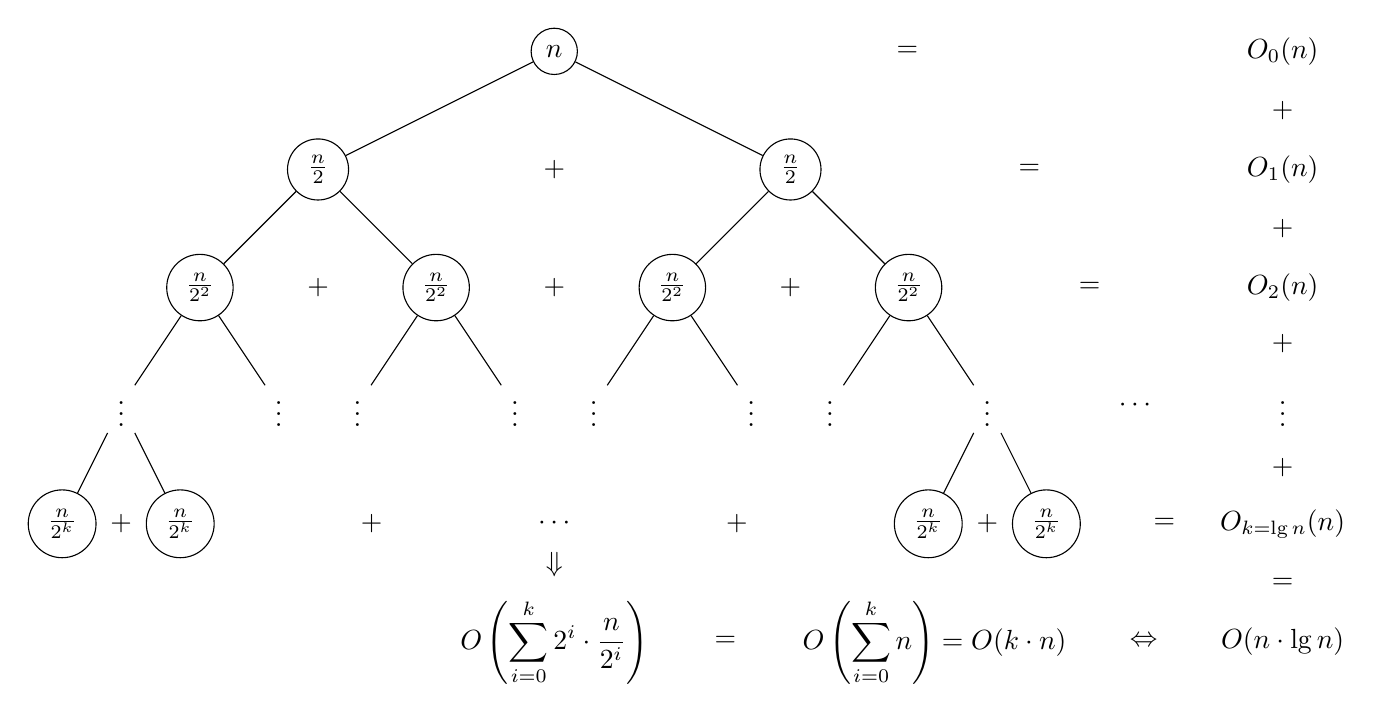
\begin{tikzpicture}[level/.style={sibling distance=60mm/#1}]
\node [circle,draw] (z){$n$}
child {node [circle,draw] (a) {$\frac{n}{2}$}
	child {node [circle,draw] (b) {$\frac{n}{2^2}$}
		child {node {$\vdots$}
			child {node [circle,draw] (d) {$\frac{n}{2^k}$}}
			child {node [circle,draw] (e) {$\frac{n}{2^k}$}}
		} 
		child {node {$\vdots$}}
	}
	child {node [circle,draw] (g) {$\frac{n}{2^2}$}
		child {node {$\vdots$}}
		child {node {$\vdots$}}
	}
}
child {node [circle,draw] (j) {$\frac{n}{2}$}
	child {node [circle,draw] (k) {$\frac{n}{2^2}$}
		child {node {$\vdots$}}
		child {node {$\vdots$}}
	}
	child {node [circle,draw] (l) {$\frac{n}{2^2}$}
		child {node {$\vdots$}}
		child {node (c){$\vdots$}
			child {node [circle,draw] (o) {$\frac{n}{2^k}$}}
			child {node [circle,draw] (p) {$\frac{n}{2^k}$}
				child [grow=right] {node (q) {$=$} edge from parent[draw=none]
					child [grow=right] {node (q) {$O_{k = \lg n}(n)$} edge from parent[draw=none]
						child [grow=up] {node (r) {$\vdots$} edge from parent[draw=none]
							child [grow=up] {node (s) {$O_2(n)$} edge from parent[draw=none]
								child [grow=up] {node (t) {$O_1(n)$} edge from parent[draw=none]
									child [grow=up] {node (u) {$O_0(n)$} edge from parent[draw=none]}
								}
							}
						}
						child [grow=down] {node (v) {$O(n \cdot \lg n)$}edge from parent[draw=none]}
					}
				}
			}
		}
	}
};
\path (a) -- (j) node [midway] {+};
\path (b) -- (g) node [midway] {+};
\path (k) -- (l) node [midway] {+};
\path (k) -- (g) node [midway] {+};
\path (d) -- (e) node [midway] {+};
\path (o) -- (p) node [midway] {+};
\path (o) -- (e) node (x) [midway] {$\cdots$}
child [grow=down] {
	node (y) {$O\left(\displaystyle\sum_{i = 0}^k 2^i \cdot \frac{n}{2^i}\right)$}
	edge from parent[draw=none]
};
\path (q) -- (r) node [midway] {+};
\path (s) -- (r) node [midway] {+};
\path (s) -- (t) node [midway] {+};
\path (s) -- (l) node [midway] {=};
\path (t) -- (u) node [midway] {+};
\path (z) -- (u) node [midway] {=};
\path (j) -- (t) node [midway] {=};
\path (y) -- (x) node [midway] {$\Downarrow$};
\path (v) -- (y)
node (w) [midway] {$O\left(\displaystyle\sum_{i = 0}^k n\right) = O(k \cdot n)$};
\path (q) -- (v) node [midway] {=};
\path (e) -- (x) node [midway] {+};
\path (o) -- (x) node [midway] {+};
\path (y) -- (w) node [midway] {$=$};
\path (v) -- (w) node [midway] {$\Leftrightarrow$};
\path (r) -- (c) node [midway] {$\cdots$};
\end{tikzpicture}

Теперд докажем с помощью \textbf{метода подстановки}, что $T(n) \leq cn\log_2n$:
\begin{description}
	\item[Базис.] $T(2) \leq c \leq c \cdot 2\log_22.$
	\item[Шаг.] Пусть утверждение доказано для всех $m \leq n$. Тогда \[T(n) \leq 2T(n/2) + cn \leq 2c(n/2)\log_2(n/2) + cn =\]
	\[= cn(\log_2n - 1) + cn = cn\log_2n.\]
\end{description}

Докажем, что $T(n) \leq kn \log_b n$ для некоторых констант $k$ и $b$ с помощью метода \textbf{частичной подстановки}. Если это так, то
\[T(n) \leq 2T(n/2) + cn \leq 2k(n/2)\log_b(n/2) + cn.\]

Кажется удобным выбрать $b = 2$. Тогда
\[T(n) \leq 2k(n/2)(\log_2n - 1) + cn = kn\log_2n - kn + cn \leq kn\log_2 n\]
при $k \geq c$.

\subsubsection{Пример 2.}

Теперь рассмотрим следующее рекуррентное соотношение: \[F(n) \leqslant F(n/2) + cn\]
Построим дерево рекурсии для данного соотношения. Легко заметить, что оно будет иметь вид $cn \to cn/2 \to cn/4 \to \ldots \to c$. На $i$-ом уровне~--- одна подзадача размера $n / 2^i$, требующая $cn / 2^i$ времени (не считая времени, уходящего на рекурсивные вызовы). Всего уровней~--- $\log_2 n$. Общее время:
\[F(n) \leq \sum_{i=0}^{\log_2n - 1}\frac{cn}{2^i} = cn\sum_{i=0}^{\log_2n - 1}\frac{1}{2^i} \leq cn \sum_{i=0}^{\infty}\frac{1}{2^i} = 2cn = O(n).\]

Докажем, что $F(n) \leq kn^d$ для некоторых констант $k$ и $d$ методом частичной подстановки. Если это так, то
\[F(n) \leq F(n/2) + cn \leq k(n/2)^d + cn = \frac{k}{2^d}n^d + cn.\]

Кажется удобным выбрать $d = 1$. Тогда $F(n) \leq \frac{kn}{2} + cn = kn$ при $k = 2c$.

Проверим, что базисное условие тоже выполняется: $F(2) \leq c \leq 2c \cdot 2$.

\subsubsection{Пример 3.}
Рассмотрим следующее рекуррентное соотношение:
\[T(n) \leq aT(n/2) + cn\]
Попробуем доказать, что $T(n) \leq kn^d$ для некоторых констант $k$ и $d$. Если это так, то
\[T(n) \leq aT(n/2) + cn \leq ak(n/2)^d + cn = \frac{a}{2^d}kn^d + cn.\]

Кажется удобным выбрать $d = \log_2 a$ так, что $a / 2^d = 1$. Однако чтобы избавиться от $cn$ в правой части вышеприведенного равенства, усилим гипотезу индукции.

Докажем, что $T(n) \leq kn^d - \ell n$ для $d = \log_2a$ и некоторых констант $k$ и $\ell$. Если это так, то
\[T(n) \leq aT(n/2) + cn \leq a(k(n/2)^d - \ell(n/2)) + cn =\]
\[= \frac{a}{2^d}kn^d - \frac{a\ell}{2}n + cn = kn^d - (\frac{a\ell}{2} - c)n = kn^d - \ell n\]
при $a\ell/2 - c = \ell$, т.е. при $\ell = 2c / (a - 2)$.

Базис: $T(2) \leq 2 \leq k \cdot 2^d - 2\ell$ при подходящем $k$.

Так как $\ell = 2c / (a - 2)$, доказательство применимо только к случаю $a > 2$. В этом случае $T(n) = O(n^{\log_2a})$.

\subsubsection{Пример 4.}
Рассмотрим следующее рекуррентное соотношение:
\[T(n) \leq 2T(n/2) + cn^2\]

Рассмотрим дерево рекурсии для данного соотношения. На $i$-ом уровне --- $2^i$ подзадач размера $n / 2^i$, каждая из которых требует $c(n/2^i)^2$ времени (не считая времени, уходящего на рекурсивные вызовы). Один уровень требует $2^ic(n / 2^i)^2 = cn^2 / 2^i$ времени. Всего уровней --- $\log_2 n$. Общее время:
\[T(n) \leq \sum_{i=0}^{\log_2n - 1}\frac{cn^2}{2^i} = cn^2\sum_{i=0}^{\log_2n - 1}\frac{1}{2^i} \leq 2cn^2 = O(n^2).\]

Докажем, что $T(n) \leq kn^d$ для некоторых констант $k$ и $d$ методом частичной подстановки. Если это так, то
\[T(n) \leq 2T(n/2) + cn^2 \leq 2k(n/2)^d + cn^2 = \frac{k}{2^{d-1}}n^d + cn^2.\]

Кажется удобным выбрать $d = 2$. Тогда
\[T(n) \leq \frac{k}{2}n^2 + cn^2 = kn^2\]
при $k = 2c$.

Базис: $T(2) \leq c \leq 2c \cdot 2^2$.

\subsection{Основная теорема о рекуррентных соотношениях. Доказательство основной теоремы.}
\begin{theorem}
	
	Пусть $a > 1$ и $b > 1$~--- константы, $f(n)$~--- функция, а $T(n)$ определена на множестве неотрицательных целых чисел с помощью рекуррентного соотношения \[T(n) = aT(n/b) + f(n),\] где $n/b$ интерпретируется либо как $\lfloor n/b \rfloor$, либо как $\lceil n/b\rceil$. Тогда Т(п) имеет следующие асимптотические границы.
	\begin{enumerate}
		\item Если $f(n) = O(n^{\log_b a - \varepsilon})$ для некоторой константы $\varepsilon > 0$, то $T(n) = \Theta(n^{\log_b a})$.
		\item Если $f(n) = \Theta(n^{\log_b a})$, то $T(n) = \Theta(n^{\log_b a}\lg n)$.
		\item Если $f(n) = \Omega(n^{\log_b a - \varepsilon})$ для некоторой константы $\varepsilon > 0$ и $af(n/b) \leqslant cf(n)$ для некоторой константы $c < 1$ и всех достаточно больших $n$, то $T(n) = \Theta(f(n))$.
	\end{enumerate}
\end{theorem}
\begin{proof}
	Доказательство этой теоремы будет разбито на две части. 
	
	В первой части анализируется данное соотношение только для точных степеней числа $b$. Анализ проводится с помощью доказательства двух лемм. В первой из них
	решение основного рекуррентного соотношения сводится к вычислению выражения, содержащего суммирование. Во второй лемме определяются границы этой суммы. В третьей лемме с помощью первых двух доказывается версия основной
	теоремы для случая, когда $n$~--- точная степень $b$.
	
	\begin{lemma}
		Пусть $a \geqslant 1$ и $b > 1$~--- константы, а $f(n)$~--- неотрицательная функция, определённая для точных степеней $b$. Определим функцию $T(n)$ на этом же множестве следующим образом:
		\[T(n) = \begin{cases}
		\Theta(1), & n = 1 \\
		aT(n/b) + f(n), & n = b^i, i > 1
		\end{cases}\]
		Тогда \[T(n) = \Theta(n^{\log_b a}) + \sum_{j = 0}^{\log_b n - 1}a^j f(n/b^j)\]
	\end{lemma}
	\begin{proof}
		Рассмотрим дерево рекурсии для данного рекуррентного соотношения. Корень дерева имеет стоимость $f(n)$, и у него $a$ дочерних ветвей, стоимость каждой из которых равна $f(n/b)$. (В ходе этих рассуждений, особенно для
		визуального представления дерева рекурсии, удобно считать число а целым, хотя это и не следует из каких-либо математических соотношений.) Каждая из этих
		дочерних ветвей, в свою очередь, также имеет $a$ дочерних ветвей (таким образом, получается, что на втором уровне дерева имеется $a^2$ узлов), время выполнения каждой из которых равно $f(n/b^2)$. Обобщая эти рассуждения, можно сказать, что на $j$-м уровне находится $a^j$ узлов, стоимость каждого из которых равна $f(n/b^j)$. Стоимость каждого листа равна $T(1) = \Theta(1)$, и все листья находятся на глубине $\log_b n$, поскольку $n/b^{\log_b n} = 1$. Всего же у дерева $a^{\log_b n} = n^{\log_b a}$ листьев.
	\end{proof}
	\begin{lemma}
		Пусть $a \geqslant 1$ и $b > 1$~--- константы, а $f(n)$~--- неотрицательная функция, определённая для точных степеней $b$. Определим функцию $g(n)$ на этом же множестве следующим образом:
		\[g(n) = \sum_{j = 0}^{\log_b n - 1}a^j f(n/b^j)\]
		Тогда её можно асимптотически оценить следующим образом:
		\begin{enumerate}
			\item Если $f(n) = O(n^{\log_b a - \varepsilon})$ для некоторой константы $\varepsilon > 0$, то $g(n) = O(n^{\log_b a})$.
			\item Если $f(n) = \Theta(n^{\log_b a})$, то $g(n) = \Theta(n^{\log_b a}\lg n)$.
			\item Если $f(n) = \Omega(n^{\log_b a - \varepsilon})$ для некоторой константы $\varepsilon > 0$ и $af(n/b) \leqslant cf(n)$ для некоторой константы $c < 1$ и всех достаточно больших $n$, то $g(n) = \Theta(f(n))$.
		\end{enumerate}
	\end{lemma}
	\begin{proof}
		Рассмотрим первый случай. Тогда получаем, что \[g(n) = O\left(\sum_{j = 0}^{\log_b n - 1}a^j \left(\frac{n}{b^j}\right)^{\log_b a - \varepsilon}\right).\]
		Оценим данную сумму в $O$-обозначениях:
		\begin{multline*}
			\sum_{j = 0}^{\log_b n - 1}a^j \left(\frac{n}{b^j}\right)^{\log_b a - \varepsilon} = n^{\log_b a - \varepsilon} \sum_{j = 0}^{\log_b n - 1} \left(\frac{ab^{\varepsilon}}{b^{\log_b a}}\right)^j = n^{\log_b a - \varepsilon} \sum_{j = 0}^{\log_b n - 1} \left(b^{\varepsilon}\right)^j = \\ = n^{\log_b a - \varepsilon} \frac{b^{\varepsilon \log_b n} - 1}{b^{\varepsilon} - 1}
			= n^{\log_b a - \varepsilon} \frac{n^{\varepsilon} - 1}{b^{\varepsilon} - 1}
		\end{multline*}
		Так как $b$~--- константа, то последнее выражение можно представить в виде $n^{\log_b a - \varepsilon}O(n^{\varepsilon}) = O(n^{\log_b a})$.
		
		Теперь рассмотрим второй случай. Согласно нему, \[g(n) = \Theta\left(\sum_{j = 0}^{\log_b n - 1}a^j \left(\frac{n}{b^j}\right)^{\log_b a}\right).\]Опять же, распишем сумму:
		\[\sum_{j = 0}^{\log_b n - 1}a^j \left(\frac{n}{b^j}\right)^{\log_b a} = n^{\log_b a} \sum_{j = 0}^{\log_b n - 1}\left(\frac{a}{b^{\log_b a}}\right)^{j} = n^{\log_b a} \sum_{j = 0}^{\log_b n - 1} 1 = n^{\log_b a} \log_b n\]
		Отсюда получаем желаемое.
		
		Далее, случай 3 доказывается аналогично. Поскольку $f(n)$ фигурирует в определении функции $g(n)$ и все члены $g(n)$ неотрицательны, можно заключить, что для точных степеней $b$ справедливо соотношение $g(n) = \Omega(f(n))$. Согласно нашему предположению из формулировки леммы, для некоторой константы $c > 1$ и всех достаточно больших $n$ выполняется неравенство $af(n/b) \leqslant cf(n)$. Повторив итерацию $j$ раз, получаем, что $a^{j}f(n/b^j) \leqslant c^jf(n)$ в предположении, что итерируемые значения достаточно велики. Поскольку последнее (и наименьшее) такое значение равно $n/b^{j - 1}$, хватит предположения о том, что оно достаточно велико.
		
		Подстановка в уравнение и упрощение приводят к геометрической прогрессии, зависящей только от $c$. Эта прогрессия убывающая, поэтому её можно ограничить сверху некоторым выражением, которое зависит только от $c$, т.е. константой. Тогда $g(n) = O(f(n)) \implies g(n) = \Theta(f(n))$.
	\end{proof}
	Дальнейшее доказательство сводится к рассмотрению трёх случаев с использованием этих лемм.
	
	На данный момент теорема доказана только для степеней числа $b$. Но выполняется ли она дла любого $n$? Сейчас мы докажем, что да, выполняется.
	
	Чтобы завершить доказательство основной теоремы, необходимо обобщить проведенный ранее анализ на случай, когда рекуррентное соотношение определено не только для точных степеней числа $b$, но и для всех целых чисел. Получить
	нижнюю границу для выражения
	\[T(n) = aT(\lceil n/b \rceil) + f(n)\]
	и верхнюю границу для
	\[T(n) = aT(\lfloor n/b \rfloor) + f(n)\]
	не составляет труда, поскольку в первом случае для получения нужного результата можно использовать неравенство $\lceil n/b \rceil \geqslant n/b$, а во втором~--- неравенство $\lfloor n/b \rfloor \leqslant n/b$. Чтобы получить нижнюю границу второго рекуррентного 
	соотношения, необходимо применить те же методы, что и при нахождении верхней границы для первого рекуррентного соотношения, поэтому здесь будет показан поиск только последней. 
	Сперва введём последовательность $n_i$ следующим образом:
	\[n_i = \begin{cases}
	n, & i = 0 \\
	\lceil n_{i - 1}/b \rceil, & i > 0
	\end{cases}\]
	Дерево рекурсии, представленное для случая точной степени, модифицируется следующим образом: на каждом уровне $n/b^i$ меняется на $n_i$. Теперь определим $k$ такое, что $n_k$~--- константа. Для этого воспользуемся неравенством $\lceil x \rceil \leqslant x + 1$:
	\[\begin{array}{c}
		n_0 \leqslant n, \\
		n_1 \leqslant \dfrac{n}{b} + 1, \\
		n_2 \leqslant \dfrac{n}{b^2} + \dfrac{1}{b} + 1, \\
		\vdots
	\end{array}\]
	Тогда получаем (с применением суммы убывающей геометрической прогрессии), что
	\[n_j < \frac{n}{b^j} + \frac{b}{b - 1}\]
	Пусть $j = \lfloor \log_b n \rfloor$. Тогда
	\[n_j < \frac{n}{b^j} + \frac{b}{b - 1} < \frac{n}{b^{\log_b n - 1}} + \frac{b}{b - 1} = \frac{1}{1/b} + \frac{b}{b - 1} = O(1)\]
	Тогда можно пользоваться аналогом формулы из первой леммы:
	 \[T(n) = \Theta(n^{\log_b a}) + \sum_{j = 0}^{\lfloor \log_b n \rfloor\ - 1}a^j f(n_j)\]
	 Докажем, что для данной суммы выполняются те же условия, что и для случая с целой степенью. Начнем со случая 3. Если $af(n/b) \leqslant cf(n)$ для $n > b + \frac{b}{b - 1}$,
	 где $c < 1$~--- константа, то $a^jf(n_jj) \leqslant c^jf(n)$ . Следовательно, сумму в можно вычислять, как в лемме 4.3. 
	 
	 В случае 2 имеем $f(n) = \Theta(n^{\log_b a})$.
	 Если мы сможем показать, что $f(n_j) = \Theta(n^{\log_b a}/a_j) = \Theta((n/b_j)^{\log_b a})$, то 
	 доказательство случая 2 леммы 4.3 будет завершено. Заметим, что из $j \leqslant \lfloor \log_b n \rfloor$
	 следует $b^j/n \leqslant 1$. Наличие границы $f(n) = O(n^{\log_b a})$ подразумевает, что 
	 существует такая константа $c > 0$, что для всех достаточно больших $n$ выполняется
	 \begin{multline*}
	 	f(n_j) \leqslant c\left(\frac{n}{b^j} + \frac{b}{b - 1}\right)^{\log_b a} = c\frac{n^{\log_b a}}{a^j}\left(1 + \frac{b^{j + 1}}{n(b -1)}\right)^{\log_b a} \leqslant c\frac{n^{\log_b a}}{a^j}\left(1 + \frac{b}{b -1}\right)^{\log_b a} = \\ = O\left(\frac{n^{\log_b a}}{a^j}\right)
	 \end{multline*}
	 поскольку $c(1 + b/(b - 1))^{\log_b a}$ представляет собой константу. Таким образом, случай 2 доказан. Доказательство случая 1 почти идентично. Ключевым моментом является доказательство границы $f(n_j) = O((n/b_j)^{\log_b a - \varepsilon})$, которое аналогично соответствующему доказательству случая 2, хотя алгебраические выкладки при
	 этом оказываются несколько более сложными.
	 
	 Итак, мы доказали соблюдение верхних границ в основной теореме для всех целых $n$. Соблюдение нижних границ доказывается аналогично.
\end{proof}

\newpage
\section{Разбиение массива по опорному элементу на три части (элементы, меньшие опорного, равные опорному и большие опорного). Оптимальность сортировки слиянием. Выбор порядковой статистики за время O(n): рандомизированный и детерминированный алгоритмы.}

\subsection{Быстрая сортировка. Продолжение}
Говоря об алгоритме быстрой сортировки (\textsc{QSort}), мы рассматривали только случаи, когда все элементы различны. Однако это далеко не всегда так. Если в входном массиве есть равные элементы, то алгоритм может застопориться. Для того, чтобы избежать этого, изменим алгоритм \textsc{Partition}. Попытаемся преобразовывать массив таким образом, чтобы в левой части стояли элементы строго меньшие опорного, в правой --- строго большие, а в середине --- равные ему:
\[\begin{array}{|c|c|c|c|c|}
	\hline
	\phantom{x}  & \dots & x & \dots & \phantom{x}  \\
	\hline
\end{array}
\longrightarrow
\begin{array}{|c|c|c|}
    \hline
    <x&=x&>x\\
    \hline
\end{array}\]

Обозначим за опорный элемент последний. Будем проходиться по массиву от начала до конца, выставляя элементы в нужном порядке (? — ещё не просмотренные элементы):
\[\begin{array}{lllll}
    \hline
   	\multicolumn{1}{|c|}{<x} & \multicolumn{1}{|c|}{>x} & \multicolumn{1}{|c|}{  ?  } & \multicolumn{1}{|c|}{=x} & \multicolumn{1}{|c|}{x}\\
    \hline
    [1, i) & [i, j) & [j, k) & [k, n) & n
\end{array}\]

\begin{algorithm}
\caption{Модифицированный алгоритм \textsc{Partition}}
\begin{algorithmic}[1]
\Function{Partition}{$a$}
\State $i \mathrel{:=} 1$
\State $j \mathrel{:=} 1$
\State $k \mathrel{:=} n - 1$
\While{$j < k$}
	\If{$a[j] = a[n]$}
		\State $k \mathrel{:=} k - 1$
		\State $a[j], a[k] \mathrel{:=} a[k], a[j]$
	\Else \If{$a[j] < a[n]$}
		\State $a[i], a[j] \mathrel{:=} a[j], a[i]$
		\State $j \mathrel{:=} j + 1$
		\State $i \mathrel{:=} i + 1$
	\Else
		\State $j \mathrel{:=} j + 1$
	\EndIf
	\EndIf
\EndWhile
\EndFunction
\end{algorithmic}
\end{algorithm}

Заметим, что $j = k$ (так как алгоритм не закончит работу до тех пор, пока это не станет верно). Тогда на выходе получится массив вида:

\[\begin{array}{lll}
    \hline
    \multicolumn{1}{|c|}{<x} & \multicolumn{1}{|c|}{>x} & \multicolumn{1}{|c|}{=x}\\
    \hline
    [1, i) & [i, j) & [k, n]
\end{array}\]

Остаётся только переставить части массива:

\begin{algorithm}
\begin{algorithmic}[1]
\State  $j \mathrel{:=} n$
\While{$i < k$ and $j \geqslant k$}
	\State $a[i], a[j] \mathrel{:=} a[j], a[i]$
	\State $i \mathrel{:=} i + 1$
	\State $j \mathrel{:=} j - 1$
\EndWhile
\end{algorithmic}
\end{algorithm}
 
\

\textbf{В:} Самая быстрая из наших сортировок --- $O(n \log n)$. А можно ли быстрее?

\textbf{О:} На основе только сравнений --- нет. 

Использовать разобранные нами сортировки можно на любых сущностях, для которых определена операция сравнения.

Предположим теперь, что мы сортируем натуральные числа, не превосходящие некоторого числа $C$.

Создадим массив $b$ размера $C$, заполненный нулями. Будем проходить по исходному массиву $a$ и на каждом шаге будем добавлять 1 к соответствующему элементу массива $b$: 
\[b[a[i]] \mathrel{:=} b[a[i]] + 1\]
Потом, проходя по получившемуся массиву $b$, будем восстанавливать исходный массив уже в отсортированном виде.

Такая сортировка будет работать за $O(n)$, однако, она не универсальна.

Вернёмся к универсальным сортировкам. Рассмотрим дерево для массива $a = [6, 5, 2]$:

\begin{center}
\begin{forest}
for tree={
	%parent anchor=south,
	%child anchor=north,
	if n children=0{
		font=\itshape,
		%tier=terminal,
	}{},
}
[{$\mathbf{a[1] < a[2]}$}
	[{$a[1] < a[3]$}
		[{$a[2] < a[3]$}
			[{$(6, 5, 2)$}
			]
			[{$(5, 6, 2)$}
			]
		]
		[{$(2, 6, 5)$}
		]
	]
	[{$\mathbf{a[2] < a[3]}$}
		[{$a[1] < a[3]$}
			[{$(5, 6, 2)$}
			]
			[{$(5, 2, 6)$}
			]
		]
		[{$\mathbf{(2, 6, 5)}$}
		]
	]
]
\end{forest}
\end{center}

Подобное дерево можно составить для любого детерминированного\footnote{Детерминированный алгоритм — алгоритмический процесс, который выдаёт предопределённый результат для заданных входных данных. Например, \textsc{QSort}, выбирающий опорный элемент случайным образом, не является детерминированным.} алгоритма сортировки, зафиксировав $n$. Сложность алгоритма будет являться высота $h$ дерева. Посчитаем это $h$:
\begin{itemize}
	\item[$\blacktriangleright$] Так как алгоритм должен работать на любой перестановке из $n$ элементов, то у дерева не может быть меньше, чем $n!$ листов.
	\item[$\blacktriangleright$] Так как сравнение --- бинарная операция, то у каждой вершины не более двух потомков. Тогда в дереве не может быть больше, чем $2^h$ листьев.
	\item[$\blacktriangleright$] Тогда $2^h \geqslant n! \iff h \geqslant \log_2 n!$.
	Заметим, что:
	\[n! = 1 \cdot 2 \cdot \ldots \cdot \left\lfloor\frac{n}{2}\right\rfloor \cdot \underbrace{ \left(\left\lfloor\frac{n}{2}\right\rfloor + 1\right) \cdot \ldots (n - 1) \cdot n}_\text{каждый из $\frac{n}{2}$ элементов не меньше $\frac{n}{2}$} \geqslant \left(\frac{n}{2}\right)^{\frac{n}{2}} \]
	Тогда $h \geqslant \log_2 \left(\frac{n}{2}\right)^{\frac{n}{2}} = \frac{n}{2} \log_2 \frac{n}{2} = \Omega(n \log n)$. Из этого следует, что отсортировать произвольный массив с помощью только сравнений меньше, чем за $\Omega(n \log n)$ операций, невозможно.
\end{itemize}

\subsection{Поиск медианы}

Медиана --- такой элемент массива, что не меньше половины элементов меньше неё, и не меньше половины --- больше.

Для отсортированного массива размера $n$ медиана будет  находиться под номером $\dfrac{n + 1}{2}$ для нечётных $n$ и $\dfrac{n}{2}$ для чётных $n$.
Пример: для массива (8, 1, 3, 5, 6, 9) медианой будет являться~5.

Как же найти медиану?
Очевидно, что можно отсортировать и взять средний --- $\Theta(n)$.

А можно ли найти медиану ли за линейное время?
Можно.
Напишем алгоритм, находящий элемент, стоящий на k-ом месте в массиве, получающемся из входного после сортировки.
Это называется поиском $k$-ой порядковой статистики.
Составим этот алгоритм, немного модифицировав QSort:

\begin{algorithm}
\caption{Поиск $k$-ой порядковой статистики}
\begin{algorithmic}[1]
\Function{Select}{$a, k$}
	\State choose pivot $a[p]$
	\State $i \mathrel{:=} \textsc{Partition}(a, p)$
	\If{$i \mathrel{:=} k$}
		\State return $a[i]$	
	\EndIf
	\If{$i > k$}
		\State return $\textsc{Select}(a[1 \ldots i - 1], k)$
	\Else
		\State return $\textsc{Select}(a[i + 1 \ldots n], k - i)$
	\EndIf
\EndFunction
\end{algorithmic}
\end{algorithm}

Как и в быстрой сортировке, неправильно выбранный опорный элемент портит скорость до $n^2$. Будем выбирать опорный элемент случайным образом. Попробуем посчитать время работы в среднем случае.

$j$-подзадача размера $n'$. $\left( \frac{3}{4} \right)^{j+1}n < n' \leqslant \left( \frac{3}{4} \right)^{j}n$

Как и в QSort, в среднем мы потратим две попытки на переход к следующему $j$.

Максимальное $j$ --- $O(\log_\frac{4}{3} n)$

$T(n) \leqslant \sum\limits_{j=0}^{\log_{\frac{4}{3}}n} 2\cdot c\cdot \left( \frac{3}{4} \right)^jn = 2cn\sum\limits_{j=0}^{\log_{\frac{4}{3}}n}\left( \frac{3}{4} \right)^j \leqslant 2cn$

Время работы алгоритма в худшем случае всё ещё $O(n^2)$.
Худший случай — когда на каждом шаге мы отщеплем всего один элемент.
Для достижения лучшего случая, на каждом шаге нужно выбирать в качестве опорного элемента медиану.

\subsection{Медиана медиан}
Попробуем несколько модифицировать наш алгоритм.
Разобьём входной массив на группы по 5 элементов.
Отсортируем каждую такую группу.
Так как размер каждой группы зафиксирован, время сортировки не зависит от $n$.
Зависит только количество сортировок.
Возьмём медиану в каждой группе и применим алгоритм нахождения медианы к получившемуся массиву медиан.
Выберем её в качестве опорного элемента.

\begin{algorithm}
\caption{Поиск $k$-ой порядковой статистики 2}
\begin{algorithmic}[1]
\Function{Select}{$a, k$}
	\State Divide a into groups of 5
	\State Choose medians $m_1,\ldots m_\frac{n}{5}$
	\State $x = \textsc{Select}([m_1,\ldots, m_\frac{n}{5}], \frac{n}{10})$
	\State choose $x$ as pivot $a[p]$
	\State $i \mathrel{:=} \textsc{Partition}(a, p)$
	\If{$i \mathrel{:=} k$}
		\State return $a[i]$	
	\EndIf	
	\If{$i > k$}
		\State return $\textsc{Select}(a[1 \ldots i - 1], k)$
	\Else
		\State return $\textsc{Select}(a[i + 1 \ldots n], k - i)$
	\EndIf
\EndFunction
\end{algorithmic}
\end{algorithm}

$T(n) \leqslant cn + T\left(\frac{n}{5}\right) + T\left( \frac{7}{10}n \right)$

$T(n) \leqslant ln$ для некоторого $l$

$T(n) \leqslant cn + T(\frac{n}{5}) + T(\frac{7}{10}) \leqslant cn + \frac{ln}{5} + \frac{7}{10}ln$
\newpage
\section{Поиск ближайшей пары точек за время O(n log n).}

Во множестве точек на прямой, заданных своими координатами, требуется найти пару точек, находящихся на наименьшем евклидовом расстоянии друг от друга. Эту задачу можно решить за время $O(n\log n)$, отсортировав точки по координатам за время $O(n\log n)$ и найдя ближайшие точки среди соседних за время $O(n)$.

Усложним задачу: точки находятся на плоскости и заданы двумя своими координатами (предположим, что у всех точек различные координаты $x$ и различные координаты $y$). Создадим два массива точек: в массиве $P_x$ все исходные точки упорядочены по координате $x$, а в массиве $P_y$ --- по координате $y$. Далее используем стратегию <<разделяй и властвуй>>.

Пусть $x^*$ --- медианная координата $x$. Разделим множество точек пополам на множества $L$ и $R$, поместив в первое множество точки с координатой $x$, не превышающей $x^*$, а во второе --- все остальные. Используя $P_x$ и $P_y$, можно за линейное время вычислить упорядочения $L$ и $R$ по обеим координатам, получив списки $L_x, L_y, R_x$ и $R_y$. В каждой половине рекурсивно найдем по паре ближайших точек.

Пусть $\delta$ --- минимальное из расстояний между найденными парами точек в каждой половине. Искомая пара точек может совпадать с одной из найденных пар, но может и состоять из точек, принадлежащих разным половинам (одна точка --- в $L$, другая --- в $R$). В последнем случае расстояние между искомой парой точек не больше $\delta$.

Рассмотрим полосу ширины $2\delta$ с центром по прямой $x = x^*$. Очевидно, что точки из разных половин, находящиеся на расстоянии не более $\delta$ друг от друга, должны находиться в этой полосе. Одним проходом по $P_y$ сформируем массив $S_y$ точек этой полосы, упорядоченный по координате $y$. Разобьем полосу на квадраты со стороной $\frac{\delta}{2}$. Две точки не могут попасть в один квадрат, так как каждый квадрат целиком находится в левой или правой половине плоскости, а расстояние между точками из одной половины не может быть меньше $\delta$. Если же две точки разделены по вертикали тремя горизонтальными рядами квадратов, то расстояние между ними превышает $\delta$. Следовательно, пары точек, находящихся друг от друга на расстоянии не больше $\delta$, стоит искать среди точек, разделенных не более чем двумя рядами квадратов. В упорядоченном по координате $y$ списке $S_y$ между такими точками может быть не более 14 других точек, так как один горизонтальный ряд содержит четыре квадрата, а в одном квадрате --- не более одной точки. Поэтому точки, находящиеся на расстоянии не более $\delta$, можно найти, просмотрев 15 соседних точек для каждой точки из $S_y$. На самом деле, можно обойтись просмотром и меньшего числа соседей, но важно, что это число константно, а значит, найти искомую пару можно за время, линейное от размера $S_y$.

Псевдокод приведен в Алгоритме \ref{algo:pair}. Расстояние между точками $p$ и $q$ обозначается как $d(p, q)$.
 
\begin{algorithm}[H]
  	\caption{\algname{ClosestPair}($P$)}
	\label{algo:pair}
	\begin{algorithmic}
		\Require Массив точек $P = [(x_1, y_1), \dots, (x_n, y_n)]$, где $x_i \neq x_j$ и $y_i \neq y_j$ при $i \neq j$.
		\Ensure Точки $(x_i, y_i)$ и $(x_j, y_j)$, $i \neq j$, находящиеся на минимальном евклидовом расстоянии друг от друга среди всех точек $P$.
		\State
		\State $P_x :=$ sort $P$ by $x$
		\State $P_y :=$ sort $P$ by $y$
		\State \Return \algname{ClosestPairRec}($P_x, P_y$)\Comment{см. Алгоритм \ref{algo:pair-rec}}
	\end{algorithmic}
\end{algorithm}

\begin{algorithm}[H]
  	\caption{\algname{ClosestPairRec}($P_x, P_y$)}
	\label{algo:pair-rec}
	\begin{algorithmic}
		\Require Массив точек $P = [(x_1, y_1), \dots, (x_n, y_n)]$, где $x_i \neq x_j$ и $y_i \neq y_j$ при $i \neq j$, упорядоченный по $x$ в $P_x$ и по $y$ --- в $P_y$.
		\Ensure Точки $(x_i, y_i)$ и $(x_j, y_j)$, $i \neq j$, находящиеся на минимальном евклидовом расстоянии друг от друга среди всех точек $P$.
		\State
		\If{$P_x \leq 3$}
			\State compute all (at most three) pairwise distances
			\Return the closest pair
		\EndIf
		\State
		\State $(x^*, y^*) := P_x[\lfloor\frac{n+1}{2}\rfloor]$\Comment{медианная точка $P_x$}
		\State $L_x := P_x[1..\lfloor\frac{n+1}{2}\rfloor]$\Comment{первая половина $P_x$}
		\State $R_x := P_x[(\lfloor\frac{n+1}{2}\rfloor + 1)..n\rfloor]$\Comment{вторая половина $P_x$}
		\State $L_y := [(x, y) \in P_y \mid x \leq x^*]$
		\State $R_y := [(x, y) \in P_y \mid x > x^*]$
		\State
		\State $(p_1, p_2) := \algname{ClosestPairRec}(L_x, L_y)$
		\State $(r_1, r_2) := \algname{ClosestPairRec}(R_x, R_y)$
		\If{$d(r_1, r_2) < d(p_1, p_2)$}
			\State $p_1, p_2 := r_1, r_2$
		\EndIf
		\State
		\State $S_y := [(x, y) \in P_y \mid |x - x^*| < d(p_1, p_2)]$\Comment{точки из полосы шириной $2\delta$}
		\State
		\For{$i := 1$ \textbf{to} $|S_y| - 1$}
			\For{$j := i + 1$ \textbf{to} $\min\{i + 15, |S_y|\}$}
				\If{$d(S_y[i], S_y[j]) < d(p_1, p_2)$}
 		   			\State $p_1, p_2 := S_y[i], S_y[j]$
				\EndIf
			\EndFor
		\EndFor
		\State
		\Return $p_1, p_2$
	\end{algorithmic}
\end{algorithm}

Оценим время работы этого алгоритма:
$$T(n) = O(n\log n) + T_{\algname{ClosestPairRec}}(n),$$
где
$$T_{\algname{ClosestPairRec}}(n) = 2 T\left(\frac{n}{2}\right) + O(n) = O(n\log n).$$
\newpage
\section{Алгоритм Карацубы для умножения целых чисел. Алгоритм Штрассена для умножения матриц.}

\subsection{Умножение чисел. Алгоритм Карацубы}

Пусть $x = \overline{x_1 x_2 \ldots x_n}$ и $y = \overline{y_1 y_2 \ldots y_n}$. Распишем их умножение в столбик:
\begin{center}
	\[
	\renewcommand{\arraystretch}{0.8}
	\arraycolsep=1pt
	\begin{array}{r}
	\times\begin{array}{rrrr}
	x_1 & x_2 & \ldots & x_n \\
	y_1 & y_2 & \ldots & y_n \\
	\hline
	\end{array}
	\\
	+\begin{array}{rrrrrrr}
	& & & z_{11} & z_{12} & \ldots & z_{1n} \\
	& & z_{21} & z_{22} & \ldots & z_{2n} & \\
	& \hdotsfor{4} & & \\
	z_{n1} & z_{n2} & \ldots & z_{nn} & & & \\
	\hline
	\end{array}
	\\
	\begin{array}{rrrrrrrr}
	z_{11} & z_{12} & \dots & \dots & \dots & \dots & z_{2n} & z_{2n+1} \\
	\end{array}
	\end{array}\]
\end{center}


Какова сложность такого умножения? Всего $n$ строк. На получение каждой строки тратится $O(n)$ операций. Тогда сложность этого алгоритма --- $nO(n) = O(n^2)$. Теперь вопрос: \emph{а можно ли быстрее?} Один из величайших математиков XX века, А.Н. Колмогоров, считал, что это невозможно.

Попробуем воспользоваться стратегией <<Разделяй и властвуй>>. Разобьём числа в разрядной записи пополам. Тогда
\[\begin{array}{c}
\times \begin{cases}
x = 10^{n/2}a + b\\
y = 10^{n/2}c + d\\
\end{cases} \\
\Downarrow\\
xy = 10^{n}ac + 10^{n/2}(ad+bc)+bd
\end{array}\]

Как видно, получается 4 умножения чисел размера $\frac{n}{2}$. Так как сложение имеет сложность $\Omega(n)$, то

\[T(n) = 4T\left( \frac{n}{2} \right) + \Theta(n)\]

Чему равно $T(n)$? Воспользуемся основной теоремой. Напомним: в общем виде неравенство
имеет вид:

\[T(n) \leqslant aT\left( \frac{n}{b} \right) + cn^d\]

В нашем случае $a = 4, b = 2, d = 1$. Заметим, что $4 > 2^1 \implies a > b^d$. Тогда $T(n) = O(n^{\log_2 4}) = O(n^2)$.

Как видно, it’s not very effective. Хотелось бы свести число умножений на каждом этапе к
трём, так как это понизит сложность до $O(n^{\log_2 3}) \approx O(n^{1.58})$Но как?

Вернёмся к началу. Разложим $(a + b)(c + d)$

\[(a+b)(c+d) = ac+(ad+bc) + bd \implies ad + bc = (a + b)(c + d) - ac - bd\]

Подставим это в начальное выражение для $xy$:

\[xy = 10^{n}ac + 10^{n/2}((a + b)(c + d) - ac - bd)+bd\]

Отсюда видно, что достаточно посчитать три числа размера $\frac{n}{2}$: $(a + b)(c + d), ac$ и $bd$. Тогда:

\[T(n) = 3T\left( \frac{n}{2} \right) + \Theta(n) \implies T(n) = O(n^{\log_2 3})\]

Полученный алгоритм называется \emph{алгоритмом Карацубы}.
На данный момент доказано, что для любого $\varepsilon > 0$ существует алгоритм, который совершает умножение двух чисел с сложностью $O(n^{1 + \varepsilon})$. Также стоит упомянуть \emph{алгоритм Шёнхаге-Штрассена}, работающий за $O(n \log n \log \log n)$

\subsection{Перемножение матриц. Алгоритм Штрассена}

Пусть у нас есть квадратные матрицы
\[A = \begin{pmatrix}
a_{11} & a_{12} & \ldots & a_{1n} \\
a_{21} & a_{22} & \ldots & a_{2n} \\
\vdots & \vdots & \ddots & \vdots \\
a_{n1} & a_{n2} & \ldots & a_{nn} \\
\end{pmatrix}
\text{и } 
B = \begin{pmatrix}
b_{11} & b_{12} & \ldots & b_{1n} \\
b_{21} & b_{22} & \ldots & b_{2n} \\
\vdots & \vdots & \ddots & \vdots \\
b_{n1} & b_{n2} & \ldots & b_{nn} \\
\end{pmatrix}\]

Сколько операций нужно для умножения матриц? Умножим их по определению. Матрицу
$C = AB$ заполним следующим образом:
\[c_{ij} = \sum\limits_{k = 1}^{n} a_{ik}b_{kj}\]

Всего в матрице $n^2$ элементов. На получение каждого элемента уходит $O(n)$ операций (умножение за константное время и сложение $n$ элементов). Тогда умножение требует $n^2O(n) = O(n^3)$
операций.

А можно ли быстрее? Попробуем применить стратегию «Разделяй и властвуй». Представим
матрицы $A$ и $B$ в виде:

\[A = \begin{pmatrix}
A_{11} & A_{12}\\
A_{21} & A_{22}
\end{pmatrix}
\text{и } 
B = \begin{pmatrix}
B_{11} & B_{12}\\
B_{21} & B_{22}
\end{pmatrix}\]
где каждая матрица имеет размер $\frac{n}{2}$. Тогда матрица $C$ будет иметь вид:
\[C = \begin{pmatrix}
A_{11}B_{11}+A_{12}B_{21} & A_{11}B_{12}+A_{12}B_{22}\\
A_{21}B_{11}+A_{22}B_{21} & A_{21}B_{12}+A_{22}B_{22}
\end{pmatrix}\]
 Как видно, получаем 8 перемножений матриц порядка $\frac{n}{2}$. Тогда

\[T(n) = 8T\left( \frac{n}{2} \right) + O(n^2)\]

По основной теореме получаем, что $T(n) = O\left(n^{\log_{2} 8}\right) = O(n^{3})$.

Можно ли уменьшить число умножений до 7? \emph{Алгоритм Штрассена} утверждает, что можно. Он предлагает ввести следующие матрицы (даже не спрашивайте, как до них дошли):

\[\begin{cases}
    M_1 = (A_{11} + A_{22})(B_{11} + B_{22}); \\
    M_2 = (A_{21} + A_{22})B_{11}; \\
    M_3 = A_{11}(B_{12} - B_{22}); \\
    M_4 = A_{22}(B_{21} + B_{11}); \\
    M_5 = (A_{11} + A_{12})B_{22}; \\
    M_6 = (A_{21} - A_{11})(B_{11} + B_{12}); \\
    M_7 = (A_{12} - A_{22})(B_{21} + B_{22}); \\
\end{cases}\]
Тогда
\[\begin{cases}
    C_1 &= M_1+M_4-M_5+M_7; \\
    C_2 &= M_3+M_5; \\
    C_3 &= M_2+M_4; \\
    C_4 &= M_1-M_2+M_5+M_6; \\
\end{cases}\]

Можно проверить что всё верно (оставим это как \sout{наказание} упражнение читателю). Сложность алгоритма:

\[T(n) = 7T\left( \frac{n}{2} \right) + O(n^2) \implies T(n) = O\left(n^{\log_{2} 7} \right)\]

На данный момент один из самых быстрых алгоритмов имеет сложность $\approx O(n^{2.3})$ (\emph{ал-
горитм Виноградова}). Но этот алгоритм быстрее только в теории — из-за астрономически
огромной константы.
\newpage
\section{Быстрое возведение в степень по модулю. Динамическое программирование: выравнивание абзаца по ширине (рекурсивное решение с меморизацией).}

\subsection{Быстрое возведение в степень}
Пусть $x = \overline{x_1 \ldots x_n}$, $y = \overline{y_1 \ldots y_n}$. Можно ли за полиномиальное время возвести число $x$ в степень $y$?

Тупо умножать $x$ на себя $y$ совершенно неоптимально --- несложно показать, что сложность алгоритма будет $O(2^n)$ (где $n$ --- число цифр в числе). При этом само число $x^y$ содержит $10^{n}n$ цифр. Получается, что один только размер результата экспоненциален, то есть полиномиальной сложности не хватит даже на вывод результата.

А если по модулю (т.е. результатом будет $x^y \pmod{p}$ для некоторого указанного $p$)? Прямое умножение всё равно достаточно медленно. Можно ли быстрее? Оказывается, что да.

\begin{algorithm}
	\caption{Быстрое возведение в степень}
	\begin{algorithmic}[1]
		\Function{Power}{$x, y, p$}\Comment{алгоритм считает $x^y \pmod{p}$}
		\If{$y = 0$}
			\State return 1
		\EndIf
		\State $t \mathrel{:=} \textsc{Power}\left(x, \lfloor\frac{y}{2}\rfloor, p \right)$
		\If{$y \equiv 0 \pmod{2}$}
			\State return $t^2$
		\Else
			\State return $xt^2$
		\EndIf
		\EndFunction
	\end{algorithmic}
\end{algorithm}

Легко понять, что глубина рекурсии для данного алгоритма равна $O(\log y) = O(n)$.

Покажем, как он работает на примере $x = 4, y = 33$: \[x^{33} = x(x^{16})^{2} = x((x^{8})^2)^2 = x(((x^4)^2)^2)^2 = x((((x^2)^2)^2)^2)^2 \].
Как видно, для возведения числа в 33-ю степень достаточно 7 умножений.

\subsection{Обратная задача}

Пусть нам известны числа $x,\ z,\ p$, каждое по $n$ цифр. Можно ли за полиномиальное время найти число $y$ такое, что $x^y = z \pmod{p}$.

Сказать сложно --- с одной стороны, такой алгоритм ещё не смогли придумать. С другой стороны, не могут доказать того, что его нет. Это всё, вообще говоря, висит на известной проблеме $\mathrm{P} \mathrel{\overset{?}{=}} \mathrm{NP}$ и подробнее мы об этом поговорим ближе к концу курса.

\subsection{Обработка текста}
Предположим, у нас есть $n$ слов, и эти слова мы хотим разместить на странице (порядок, разумеется, не меняя --- это же, в конце концов, текст). При этом, шрифт моноширинный, а ширина строки ограничена. Что мы хотим --- разместить текст так, чтобы он был выровнен по обоим краям. При этом хотелось бы, чтобы пробелы были примерно одинаковы по ширине.

Введём такую ??? (меру? хз): $\varepsilon(i, j) = L-\sum\limits_{t=i}^j|w_t|-(j-i)$ --- число дополнительных пробелов в строке с $i$-го по $j$-ое слово.

Также введём $c(i, j)$ --- стоимость размещения.

\[
    c(i, j) = \begin{cases}
        +\infty, \varepsilon(i, j) < 0\\
        \left( \frac{\varepsilon(i, j)}{j-i} \right)^3, \varepsilon(i, j) \geqslant 0\\
    \end{cases}
\]

И как это решать? Можно попробовать жадным алгоритмом --- просто ``впихивать'' слова в строку, пока влезают. Он тут не работает, так как он вообще не учитывает стоимость.

Попробуем наш извечный ``разделяй и властвуй''. Базовый случай --- слова помещаются в одну строку, а если не помещаются --- переносим и повторяем. Но тут тоже не учитывается стоимость, так что вряд ли будет сильно лучше.

Вход: $w_1, \ldots, w_n; c(i, j)$.

Выход: $j_0, \ldots, j_{l+1}$, такие что $j_0 = 1,\ j_{l+1} = n,\ \sum c(j_i, j_{i+1})$ минимальна.

Сколько всего таких наборов? Мест, где в принципе может оказаться разрып строки --- $n-1$, в каждом можно поставить или не поставить --- итого $2^{n-1}$ разбиений.

Пусть $OPT(j)$ --- стоимость оптимального размещения слов с $j$-ого по $n$-ное. Наша задача --- вычислить $OPT(1)$. А как?

\[
    OPT(1) = \min\limits_{i\leqslant n}\{c(1, i)+OPT(i+1)\}
\]

\begin{lstlisting}
OPT(j):
    if j = n+1 then return 0
    f:= +inf
    for i:= j to n do
     f:= min(f, c(i, j)+OPT(i+1))
\end{lstlisting}

$(*)\ \mathrm{OPT}(3) =\begin{cases}
    0, & j>n\\
    \min\limits_{i = j\ldots n}\left\{ c(j, i) + \mathrm{OPT}(3)(i+1) \right\}, & \text{иначе}
\end{cases}$

А сложность? Построив дерево, заметим, что $\mathrm{OPT}(3)$ вычисляется два раза; $\mathrm{OPT}(4)$ -- три раза и так далее.

Будем сохранять результаты:

\begin{algorithmic}
	\Function{OPT\_cache}{$t$}
	\If{$M[j] \neq \textrm{NULL}$}
	\Else
		\State $M[j] \mathrel{:=} \textsc{OPT}(j)$
	\EndIf
	\State return $M[j]$
	\EndFunction
\end{algorithmic}

Такая методика называется \emph{динамическим программированием}.

Основная идея --- каждая задача зависит от полиномиального числа других задач.
\newpage
\section{Динамическое программирование. Задача о планировании взвешенных интервалов: рекурсивное решение с мемоизацией и итеративное решение. Свойства задач, эффективно решаемых при помощи динамического программирования: наличие полиномиального числа подзадач, выразимость исходной задачи в терминах подзадач, сводимость больших подзадач к полиномиальному числу меньших подзадач. Выравнивание абзаца по ширине: итеративное решение.}

\subsection{Продажа земли}

Предположим, что у нас есть участок земли у берега и мы хотим его продать.
При этом у нас есть несколько покупателей и каждый из них готов отдать некоторую сумму за некоторый фрагмент участка.
Как максимизировать выгоду?

Формализуем: у нас есть $n$ предложений и каждое характеризуется тремя числами — началом $s$, концом $f$ и весом $w$.
Таким образом, вход выглядит так:

$s_1, \ldots, s_n$ --- начала

$f_1, \ldots, f_n$ --- концы

$w_1, \ldots, w_n$ --- веса\\

Пример:

\includegraphics[width=5cm]{09_intervals.png}\\

На выходе мы хотим получить максимальную сумму весов непересекающихся интервалов:

\[
\max\limits_{T\subseteq \left\{ 1,\ldots, n \right\}} \sum\limits_{i\in T}w_i 
\]
\[
T: \forall i<j \implies f_i \leqslant s_j \lor f_j \leqslant s_i
\]

Перебором задача решается за $O(2^n)$

Давайте в качестве первого шага отсортируем по правым концам за $O(n\log n)$.

Введём обозначения:

O --- оптимальное решение

$OPT(i)$ — максимальаня стоимость оптимального решения для первых $i$ интервалов

$OPT(n)$ — Максимальная стоимость оптимального решения длв всех интервалов\\

Пример:

\[
    \mathrm{OPT}(6) = \max\begin{cases}
        \mathrm{OPT}(5), 6\not\in O;\\
        2+ \mathrm{OPT}(3), 6\not\in O; \text{(так как все до третьего не пересекаются с шестым)}
    \end{cases}
\]

Пусть $p(j) = \max\left\{ i<j \mid f_{i}\leqslant s_j\right\}$ --- первый интервал до $j$-го, совместимый с ним (то есть не пересекающийся).

Эффективное вычисление $p$ остается в качестве упражнения.

Тогда общая формула для $OPT$ такова:
\[
    \mathrm{OPT}(i) = \max\begin{cases}
        \mathrm{OPT}(i-1);\\
        w_i+ \mathrm{OPT}(p(i));
    \end{cases}
\]


\begin{algorithm}
	\caption{Подсчёт $OPT(i)$}
	\begin{algorithmic}[1]
		\Function{ComputeOpt}{i}
			\If{$i = 0$}
				\State return 0
			\EndIf
			\State return $\max \{\textsc{ComputeOpt}(i - 1), w_i + \textsc{ComputeOpt}(p(i))\}$
		\EndFunction
	\end{algorithmic}
\end{algorithm}

Считая, что данные уже отсортированы, получим что сложность равна $O(n)$, но только если мы сохраняем результаты вычислений.
Иначе мы делаем много лишних вычислений, и время будет таким: $T(n) = T(n-1)+T(n-2)+c$.
Очень похоже на числа Фибоначчи, а они растут экспоненциально; это выражение --- тоже.


Значит надо сохранять вычисления в некоторый массив OPT.
Инициализируем его так: 
\[
\mathrm{OPT} = [0, -1, \ldots, -1]
\]

\begin{algorithm}
	\caption{Модифицированный подсчёт $OPT(i)$}
	\begin{algorithmic}[1]
		\Function{ComputeOpt}{i}
			\If{$OPT(I) < 0$}
				\State $OPT[i] = \max \{\textsc{ComputeOpt}(i - 1), w_i + \textsc{ComputeOpt}(p(i))\}$
			\EndIf
			\State return $OPT[i]$
		\EndFunction
	\end{algorithmic}
\end{algorithm}

Вот теперь сложность алгоритма --- $O(n)$

Так как мы вычисляем 1 раз каждый элемент $OPT$, мы можем избавиться от рекурсии:\\

\begin{algorithm}
	\caption{Модифицированный подсчёт $OPT(i)$ без рекурсии}
	\begin{algorithmic}[1]
		\Function{ComputeOpt}{i}
			\State $OPT = [0, -1, \ldots, -1]$
			\For{$OPT(I) < 0$ \textbf{to} $n$}
				\State $OPT[i] = \max \{OPT[i - 1], w_i + OPT[p(i)]\}$
			\EndFor
			\State return $OPT[n]$
		\EndFunction
	\end{algorithmic}
\end{algorithm}

Как теперь определить, какие именно участки нужно продать?
Можно хранить в $OPT$ на $i$-ом месте необходимые участки, но это замедлит нашу программу (не асимптотически), так как придётся тратить на запись не константное время, а некоторое $O(n)$.
Однако, можно восстановить номера участков по массиву $OPT$:

\begin{algorithm}
	\caption{Восстановление решения}
	\begin{algorithmic}
		\Function{FindSolution}{OPT}
			\State $T = \emptyset$
			\State $i = n$
			\While{$i > 0$}
				\If{$OPT[i - 1] > w_i + OPT[p(i)]$}
					\State $i = i - 1$
				\Else
					\State $T = T \cup {i}$
					\State $i = p(i)$
				\EndIf
			\EndWhile
			\State return $p(i)$
		\EndFunction
	\end{algorithmic}
\end{algorithm}

\subsection{В общем о динамическом программировании}
Чем оно отличается от ``Разделяй и властвуй''? А тем, что задачи могут пересекаться. Ведь при использовании классического ``разделяй и властвуй'' мы бы получили экспоненциальное решение. 

Для эффективного использования этого принципа необходимы следующие условия:
\begin{itemize}
    \item Небольшое число задач; например, полиномиальное;
    \item Возможность их упорядочить и выразить решения следующих через предыдущие.
\end{itemize}

\subsection{Задача с прошлой лекции --- выравнивание текста}

Дано:\\
$w_1,\ldots, w_n$ --- длины слов.

$c(i, j)$ --- штраф за размещение $w_i,\ldots, w_j$ на одной строке.\\

Преобразуем наше рекурсивное решение в итеративное.

OPT$(i)$ --- оптимальное размещение $w_i, \ldots, w_n$.

OPT(i) = $\min\limits_{i\leqslant j\leqslant n} \left\{ c(i, j)+ \mathrm{OPT}(j+1) \right)\}$.\\

Запишем итеративный алгоритм для этой формулы.
Так как $i$-ая задача зависит от задач с большим индексом, будем заполнять массив с конца.

\begin{algorithm}
	\caption{Выравнивание текста}
	\begin{algorithmic}
		\Function{ComputeOpt}{$w_1, \ldots, w_n$}
			\State $best = [0] \times n$
			\State $OPT = [+\infty] \times (n + 1)$
			\State $OPT[n + 1] = 0$
			\For{$i \mathrel{:=} n$ \textbf{downto} 1}
				\For{$j \mathrel{:=} i$ \textbf{to} n}
					\If{$c(i, j) + OPT[j + 1] \leqslant OPT[i]$}
						\State $OPT[i] = c(i, j) + OPT[j + 1]$
						\State $best[i] = j$
					\EndIf
				\EndFor
			\EndFor
			\State return $OPT[i]$
		\EndFunction
	\end{algorithmic}
\end{algorithm}

Как видно, в данном алгоритме решение строится по ходу, потому что в данном случае это допустимо.

\newpage
\section{Вычисление редакционного расстояния и выравнивание последовательностей.}

\emph{Редакционное расстояние} $d(s, t)$ между двумя строками $s$ и $t$ --- минимальное число вставок, удалений и замен символов, позволяющих преобразовать $s$ в $t$. Расстояние между двумя строками можно задать при помощи \emph{выравнивания}. Например:

\begin{center}
\begin{tabular}{ccccccccccccccc}
	и&с&к&у&с&с&т&в&&&е&н&н&ы&й\\
	и&н&&&&&т&е&л&л&е&к&т
\end{tabular}
\end{center}

Если $|s| = |t| = n$, то число возможных выравниваний не меньше $2^n$. Действительно, выравнивание можно задать подмножеством символов строки $s$, подлежащих замене, и подмножеством  символов строки $t$, используемых при замене. Очевидно, что число возможных выравниваний равно \[\sum_{j=0}^n \binom{n}{j}^2.\]
Выравнивание можно задать и иначе, указав $k$ символов строки $s$, подлежащих замене, и $n - k$ символов строки $t$, которые должны быть вставлены. Тогда получим, что число выравниваний равно\[\binom{2n}{n}.\]

Решить задачу нахождения оптимального выравнивания можно, разбив строку $s$ на две подстроки $s_1$ и $s_2$, вычислив разбиение строки $t$ на подстроки $t_1$ и $t_2$, соответствующее оптимальному выравниванию, и решив задачу выравнивания для $s_1$ и $t_1$ и отдельно для $s_2$ и $t_2$.

Есть три возможности для выравнивания первых символов $s$ и $t$:
\begin{enumerate}
	\item $s_1 = s[0], s_2 = s[1:], t_1 = \epsilon, t_2 = t$,
	\item $s_1 = \epsilon, s_2 = s, t_1 = t[0], t_2 = t[1:]$,
	\item $s_1 = s[0], s_2 = s[1:], t_1 = t[0], t_2 = t[1:]$,
\end{enumerate}
где $\epsilon$ --- пустая строка.
Эти три выравнивания задают следующие расстояния между $s$ и $t$: 
\begin{enumerate}
	\item $d(s[1:], t) + 1$,
	\item $d(s, t[1:]) + 1$,
	\item $d(s[1:], t[1:]) + (s[0] \neq t[0])$,
\end{enumerate}
где значением $(s[0] \neq t[0])$ является 1, если $s[0] \neq t[0]$, и 0 в противном случае. Тогда
\[d(s, t) = \min\{d(s[1:], t) + 1, d(s, t[1:]) + 1, d(s[1:], t[1:]) + (s[0] \neq t[0])\}.\]

Приведенная формула дает простой рекурсивный алгоритм, вычисляющий $d(s, t)$, но чтобы гарантировать полиномиальное время работы, необходимо запоминать решения подзадач, возникающих на различных уровнях рекурсии. Если $|s| = |t| = n$, число таких подзадач равно $O(n^2)$: строка длины $n$ может быть разбита на две подстроки $n + 1$ способом.

\newpage
\section{Графы: обход в глубину и в ширину, поиск компонент связности в неориентированных графах.}

\subsection{Поиск в ширину.}

Пусть задан граф $G = (V,\ E)$ и выделена \textbf{исходная вершина} $s$. Алгоритм поиска в ширину систематически обходит все рёбра $G$ для открытия всех вершин, достижимых из $s$, вычисляя при этом расстояние (минимальное количество рёбер) от $s$ до каждой достижимой из $s$ вершины. 

Поиск в ширину имеет такое название потому, что в процессе обхода мы идём вширь, то есть, перед тем, как приступить к поиску вершин на расстоянии $k + 1$, выполняется обход всех вершин на расстоянии $k$.

На вход алгоритма подаётся заданный граф (невзвешенный), и номер стартовой вершины $s$. Граф может быть как ориентированным, так и неориентированным, для алгоритма это не важно.

Сам алгоритм можно понимать как процесс "открывания" графа: на нулевом шаге открываем только вершину $s$. На каждом следующем шаге открываем всех соседей открытой вершины соседей; т.е. за одну итерацию алгоритма происходит расширение "кольца открытий" в ширину на единицу.

Более строго это можно представить следующим образом. Создадим очередь $q$, в которую будут помещаться горящие вершины, а также заведём булевский массив $discovered[]$, в котором для каждой вершины будем отмечать, горит она уже или нет (или иными словами, была ли она посещена).

Изначально в очередь помещается только вершина $s$, и $discovered[s] = true$, а для всех остальных вершин $discovered[] = false$. Затем алгоритм представляет собой цикл: пока очередь не пуста, достать из её головы одну вершину, просмотреть все рёбра, исходящие из этой вершины, и если какие-то из просмотренных вершин ещё не горят, то поджечь их и поместить в конец очереди.

В итоге, когда очередь опустеет, обход в ширину обойдёт все достижимые из $s$ вершины, причём до каждой дойдёт кратчайшим путём. Также можно посчитать длины кратчайших путей (для чего просто надо завести массив длин путей $distance[]$), и компактно сохранить информацию, достаточную для восстановления всех этих кратчайших путей (для этого надо завести массив "предков" $parent[]$, в котором для каждой вершины хранить номер вершины, по которой мы попали в эту вершину).

Псевдокод:

\begin{algorithm}
  	\caption{\algname{BFS}($(V, E), s$)}
    \begin{algorithmic}
		\Require Граф $(V, E)$ и вершина $s \in V$.
		\Ensure Массив $distance$, где $distance[i]$ содержит расстояние от $s$ до $i$, и массив $parent$, в котором для каждой вершины хранить номер вершины, по которой мы попали в эту вершину.
		\For {$v \in V$}
			\State $discovered[v] := \textbf{False}$
			\State $distance[v] = \infty$
			\State $parent[v] = -1$
		\EndFor
		\State $discovered[s] := \textbf{True}$
		\State $distance[s] = 0$
        \State $Q := [s]$
        \While{$Q\ \textbf{is not empty}$}
            \State $u = extract(Q)$
            \State $discovered[u] = true$
            \For{$v\ :\ (u,\ v) \in E$}
                \If{$\textbf{not}\ discovered[v]$}
                    \State $discovered[v] = true$
                    \State $enqueue(v,\ Q)$
                    \State $distance[v] = distance[u] + 1$
                    \State $parent[v] = u$
                \EndIf
            \EndFor
        \EndWhile
		\State
		\Return $distance,\ parent$
	\end{algorithmic}
\end{algorithm}

\paragraph{Корректность}

\begin{theorem}
    Выполнено следующее:
    \begin{enumerate}
        \item В очереди поиска в ширину расстояние вершин до s монотонно неубывает.
        \item Алгоритм поиска в ширину в невзвешенном графе находит длины кратчайших путей до всех достижимых вершин.
    \end{enumerate}
\end{theorem}
\begin{proof}
\begin{enumerate}
    \item Докажем это утверждение индукцией по числу выполненных алгоритмом шагов.
    \begin{itemize}
        \item База: изначально очередь содержит только одну вершину $s$ с расстоянием 0, утверждение верно.
        \item Переход: пусть после $l$-ого шага алгоритма очередь содержит $p$ вершин с расстоянием $k$ и $q$ вершин с расстоянием $k + 1$. Тогда на $l+1$-ом шаге мы извлечем из очереди одну вершину и добавим в нее все непосещенные($r$ вершин), связанные с ней; расстояние до них, очевидно, будет равно $k + 1$. У нас останется $p - 1$ (возможно, 0) вершин с расстоянием $k$ и $q + r$ вершин с расстоянием $k + 1$, что соответствует нашему инварианту.
    \end{itemize}
    \item Допустим, что второе утверждение не выполнено. Выберем из вершин, для которых кратчайшие пути от $s$ найдены некорректно, ту, настоящее расстояние до которой минимально. Пусть это вершина $u$, и она имеет своим предком в дереве обхода в ширину $v$, а предок в кратчайшем пути до $u$ — вершина $w$.

    Так как $w$ — предок $u$ в кратчайшем пути, то $\rho(s,\ u) = \rho(s,\ w) + 1 > \rho(s,\ w)$, и расстояние до $w$ найдено верно, $\rho(s,\ w) = distance[w]$. Значит, $\rho(s,\ u) = distance[w] + 1$.

    Так как $v$ — предок $u$ в дереве обхода в ширину, то $distance[u] = distance[v] + 1$.

    Расстояние до $u$ найдено некорректно, поэтому $\rho(s,\ u) < distance[u]$. Подставляя сюда два последних равенства, получаем $distance[w] + 1 < distance[v] + 1$, то есть, $distance[w] < distance[v]$. Из ранее доказанной леммы следует, что в этом случае вершина $w$ попала в очередь и была обработана раньше, чем $v$. Но она соединена с $u$, значит, $v$ не может быть предком $u$ в дереве обхода в ширину, мы пришли к противоречию, следовательно, найденные расстояния до всех вершин являются кратчайшими.
\end{enumerate}
\end{proof}
\paragraph{Применение}
\begin{itemize}
    \item Поиск кратчайшего пути в невзвешенном графе.
    \item Поиск компонент связности в графе за $O(n+m)$. Для этого мы просто запускаем обход в ширину от каждой вершины, за исключением вершин, оставшихся посещёнными ($discovered=true$) после предыдущих запусков. Таким образом, мы выполняем обычный запуск в ширину от каждой вершины, но не обнуляем каждый раз массив $discovered[]$, за счёт чего мы каждый раз будем обходить новую компоненту связности, а суммарное время работы алгоритма составит по-прежнему $O(n+m)$ (такие несколько запусков обхода на графе без обнуления массива $used$ называются серией обходов в ширину).
    \item Нахождения решения какой-либо задачи (игры) с наименьшим числом ходов, если каждое состояние системы можно представить вершиной графа, а переходы из одного состояния в другое — рёбрами графа. Классический пример — игра, где робот двигается по полю, при этом он может передвигать ящики, находящиеся на этом же поле, и требуется за наименьшее число ходов передвинуть ящики в требуемые позиции. Решается это обходом в ширину по графу, где состоянием (вершиной) является набор координат: координаты робота, и координаты всех коробок.
    \item Нахождение кратчайшего пути в 0-1-графе (т.е. графе взвешенном, но с весами равными только 0 либо 1): достаточно немного модифицировать поиск в ширину: если текущее ребро нулевого веса, и происходит улучшение расстояния до какой-то вершины, то эту вершину добавляем не в конец, а в начало очереди.
    \item Нахождение кратчайшего цикла в ориентированном невзвешенном графе: производим поиск в ширину из каждой вершины; как только в процессе обхода мы пытаемся пойти из текущей вершины по какому-то ребру в уже посещённую вершину, то это означает, что мы нашли кратчайший цикл, и останавливаем обход в ширину; среди всех таких найденных циклов (по одному от каждого запуска обхода) выбираем кратчайший.
    \item Найти все рёбра, лежащие на каком-либо кратчайшем пути между заданной парой вершин $(a,\ b)$. Для этого надо запустить 2 поиска в ширину: из $a$, и из $b$. Обозначим через $distance_a[]$ массив кратчайших расстояний, полученный в результате первого обхода, а через $distance_b[]$ — в результате второго обхода. Теперь для любого ребра $(u,\ v)$ легко проверить, лежит ли он на каком-либо кратчайшем пути: критерием будет условие $distance_a[u] + 1 + distance_b[v] = distance_a[b]$.
\end{itemize}

\subsection{Поиск в глубину}

Стратегия поиска в глубину заключается в том, чтобы идти вглубь графа насколько это возможно. При выполнении поиска в глубину он исследует все рёбра, выходящие из вершины, открытой последней, и покидает вершину, только когда не остаётся неисследованных рёбер -- происходит откат в вершину, из которой была окрыта данная вершина $v$. Этот процесс продолжается до тех пор, пока не будут открыты все вершины, достижимые из исходной. Если при этом остаются неоткрытые вершшины, то одна из них выбирается в качестве новой исходной и поиск повторяется уже из неё. Этот процесс повторяется до тех пор, пока не будут окрыты все вершины.

Псевдокод:

\begin{algorithm}
  	\caption{\algname{DFS}($(V, E),\ now,\ discovered[]$)}
	\label{algo:dfs}
	\begin{algorithmic}
		\Require Граф $(V, E)$ и вершина $now \in V$.
		\Ensure Алгоритм может возвращать всё, что нужно -- высоту поддерева, длину пути, количество потомков в поддереве и т.п.
		\State
		\State $discovered[now] = \textbf{True}$
		\For{$(now,\ v) \in E}$\Comment{идём по всем соседям вершины}
		    \If{\textbf{not}\ $discovered[v]$}
		        \State DFS($(V,\ E),\ v,\ discovered$)
		        \State \Comment{Далее можно делать дополнительные махинации}
		    \EndIf
		 \EndFor
		\State
		\Return \Comment{Что необходимо.}
	\end{algorithmic}
\end{algorithm}

\paragraph{Корректность}

Поиск в глубину попросту обходит все вершины графа. Он не может зайти в уже посещённые вершины ($discovered$), значит, обойдёт каждую вершину конкретной компоненты ровно 1 раз. Алгоритм будет когда-то завершён, так как все вершины будут посещены, и в худшем случае потребуется  $O(|V|)$ запусков $DFS$.

\paragraph{Применение}

\begin{itemize}
    \item Поиск любого пути в графе.
    \item Поиск лексикографически первого пути в графе.
    \item Проверка, является ли одна вершина дерева предком другой:
        В начале и конце итерации поиска в глубину будет запоминать "время" захода и выхода в каждой вершине. Теперь за $O(1)$ можно найти ответ: вершина $i$ является предком вершины $j$ тогда и только тогда, когда $start_i < start_j$ и $end_i > end_j$.
    \item Задача LCA (наименьший общий предок).
    \item Топологическая сортировка:
        Запускаем серию поисков в глубину, чтобы обойти все вершины графа. Отсортируем вершины по времени выхода по убыванию - это и будет ответом.
    \item Проверка графа на ацикличность и нахождение цикла
    \item Поиск компонент сильной связности:
        Сначала делаем топологическую сортировку, потом транспонируем граф и проводим снова серию поисков в глубину в порядке, определяемом топологической сортировкой. Каждое дерево поиска - сильносвязная компонента.
    \item Поиск мостов:
        Сначала превращаем граф в ориентированный, делая серию поисков в глубину, и ориентируя каждое ребро так, как мы пытались по нему пройти. Затем находим сильносвязные компоненты. Мостами являются те рёбра, концы которых принадлежат разным сильносвязным компонентам.
\end{itemize}

\subsection{Компоненты связности}

Для поиска компонент связности, вообще говоря, можно использовать любой алгоритм обхода графа:
\newpage
\section{Оценка сложности алгоритмов поиска в ширину и в глубину.}

\subsection{Сложность поиска в ширину}
Вариант обхода графа в ширину из вершины $s$ приведен ниже.

\begin{algorithm}
  	\caption{\algname{BFS}($(V, E), s$)}
    \begin{algorithmic}
		\Require Граф $(V, E)$ и вершина $s \in V$.
		\Ensure Массив $distance$, где $distance[i]$ содержит расстояние от $s$ до $i$, и массив $parent$, в котором для каждой вершины хранить номер вершины, по которой мы попали в эту вершину.
		\For {$v \in V$}
			\State $discovered[v] := \textbf{False}$
			\State $distance[v] = \infty$
			\State $parent[v] = -1$
		\EndFor
		\State $discovered[s] := \textbf{True}$
		\State $distance[s] = 0$
        \State $Q := [s]$
        \While{$Q\ \textbf{is not empty}$}
            \State $u = extract(Q)$
            \State $discovered[u] = true$
            \For{$v\ :\ (u,\ v) \in E$}
                \If{$\textbf{not}\ discovered[v]$}
                    \State $discovered[v] = true$
                    \State $enqueue(v,\ Q)$
                    \State $distance[v] = distance[u] + 1$
                    \State $parent[v] = u$
                \EndIf
            \EndFor
        \EndWhile
		\State
		\Return $distance,\ parent$
	\end{algorithmic}
\end{algorithm}

Если граф представлен в виде матрицы смежности, обход в ширину занимает время $\Theta(n^2)$, так как на перебор соседей одной вершины уходит время $\Theta(n)$. Однако при использовании списков смежности на обход соседей вершины $u$ требуется время $\Theta(deg(u))$, а на обход соседей всех вершин --- время $\Theta(m)$. В этом случае общее время работы алгоритма --- $\Theta(m + n)$. 


Вызывая \algname{BFS}($(V, E), s$), мы обходим только вершины, достижимые из $s$. Обойти весь граф можно, последовательно вызывая алгоритм для всех еще не <<обнаруженных>> вершин графа, при каждом следующем запуске используя предыдущий массив $discovered$. Время обхода всего графа при использовании списков смежности --- $\Theta(m + n)$.

При практической реализации этого алгоритма вместо множеств $L[i]$ лучше использовать очередь для хранения уже обнаруженных вершин, соседи которых еще не просмотрены.

\subsection{Сложность поиска в глубину}
Вариант обхода графа в глубину из вершины $s$ (в цикле -- $now$) приведен ниже. Время работы цикла равно числу итераций в циклах $\textbf{for}$. Поскольку каждая вершина будет рассмотрена не более чем один раз -- $O(|V|)$, но при этом граф проверит все инцидентные рёбра для каждой из попавших в $\textbf{for}$ непосещённых вершин -- $O(|E|)$. Тогда сложность поиска в глубину --- $O(|V| + |E|)$.

\begin{algorithm}
  	\caption{\algname{DFS}($(V, E),\ now,\ discovered[]$)}
	\label{algo:dfs}
	\begin{algorithmic}
		\Require Граф $(V, E)$ и вершина $now \in V$.
		\Ensure Алгоритм может возвращать всё, что нужно -- высоту поддерева, длину пути, количество потомков в поддереве и т.п.
		\State
		\State $discovered[now] = \textbf{True}$
		\For{$(now,\ v) \in E}$\Comment{идём по всем соседям вершины}
		    \If{\textbf{not}\ $discovered[v]$}
		        \State DFS($(V,\ E),\ v,\ discovered$)
		        \State \Comment{Далее можно делать дополнительные махинации}
		    \EndIf
		 \EndFor
		\State
		\Return \Comment{Что необходимо.}
	\end{algorithmic}
\end{algorithm}

\newpage
\section{Способы представления графов: матрица смежности и списки смежности.}

\subsection{Матрица смежности}

Представление графа $G = (V,\ E)$ с помощью \textbf{матрицы смежности} предполагает, что вершины занумерованы в некотором порядке числами $1,\ 2,\ldots,\ |V|$. В таком случае представление графа с использованием матрицы представляет собой матрицу $A = (a_{ij})$ размера $|V| \times |V|$, такую, что
\[a_{ij} = \begin{cases}1,\ (i,\ j) \in E \\ 0,\ (i,\ j)\notin E\end{cases}\]
Если в графе разрешены кратные ребра, то значение $a_{ij}$ равно количеству ребер из $i$ в $j$.

Матрицы смежности легко адаптировать для \textbf{взвешенных графов} -- графов, с каждым ребром которого связан определённый \textbf{вес}, определяемый весовой функцией $w : E \to \R$.

Пусть $G = (V,\ E)$ -- взвешенный граф с весовой функцией $w$. Тогда будем хранить вес $w(u,\ v)$ каждого ребра $(u,\ v)\in E$ в строке $u$ и столбце $v$ матрицы смежности.

В графе с весами на ребрах  значение $a_{ij}$ равно весу ребра из $i$ в $j$. Если граф неориентированный, его матрица смежности симметрична. Если в графе нет петель, на диагонали стоят нули.

Матрица смежности всегда занимает $\Theta(|V|^2)$ памяти.

\subsection{Списки смежности}

Имеется граф $G = (V,\ E)$. Представление графа в виде \textbf{списка смежности} использует массив $Adj$ из $|V|$ списков, по одному для каждой вершины графа. Для каждой вершины $u \in V$ список $Adj[u]$ содержит все вершины $v$ такие, что $(u,\ v) \in E$, то есть, $Adj[u]$ состоит из всех смежных с $u$ вершин (можно хранить как сами номера вершин, так и указатели на них). Вершины хранятся в произвольном порядке.

Если граф ориантированный, то сумма длин всех списков смежности равна $|E|$, поскольку ребру $(u,\ v)$ однозначно соответствует элемент $v$ в списке $Adj[u]$. Если $G$ -- неориентированный граф, то сумма длин всех списков смежности равна $2|E|$, поскольку ребро $(u,\ v)$, будучи неориентированным, появляется в списке $Adj[u]$ как $v$ и в списке $Adj[v]$ как $u$. Однако, как для ориентированных, так и для неориентирванных, представляение в виде списков смежности требует объём памяти, равный $\Theta(V + E)$.

Списки смежности легко адаптировать для \textbf{взвешенных графов} -- графов, с каждым ребром которого связан определённый \textbf{вес}, определяемый весовой функцией $w : E \to \R$.

Пусть $G = (V,\ E)$ -- взвешенный граф с весовой функцией $w$. Тогда будем хранить вес $w(u,\ v)$ каждого ребра $(u,\ v)\in E$ вместе с вершиной $v$ в списке смежности $Adj[u]$.

Недостаток данного метода хранения графов заключается в том, что приходится долго определять, есть ли ребро $(u,\ v)$ в графе -- приходится пробегаться по массиву $Adj[u]$. Данная проблема, однако, решается путём составления матрицы смежности.

\subsection{Асимптотика}

Проверку на то, существует ли ребро из вершины $i$ в вершину $j$, в матрице смежности можно осуществить за $O(1)$, а в списках смежности --- за $O(deg(i))$, где $deg(i)$ --- степень вершины $i$.

Граф называют \emph{плотным}, если $|E| = \Theta(|V^2|)$, и \emph{разреженным}, если $|E| = \Theta(|V|)$. Возможны промежуточные варианты.

С другой стороны, перебор соседей вершины $i$ в матрице смежности требует время $\Theta(|V|)$, а в списках смежности --- $\Theta(deg(i))$, что обычно существенно меньше $\Theta(|V|)$ в случае разреженного графа.

\newpage
\section{Топологическая сортировка за линейное время: алгоритмы, основанные на удалении вершин без входящих ребер и на поиске в глубину. }

\textbf{Топологическая сортировка} ориентированного ациклического графа $G = (V,\ E)$ представляет собой такое линейное упорядочение всех его вершин, что если граф $G$ содержит ребро $(u,\ v)$, то $u$ при таком упорядочении располагается до $v$ (в случае цикла такая сортировка невозможна).

Псевдокод:

\begin{algorithm}
  	\caption{\algname{Topsort}($(V, E)$)}
	\begin{algorithmic}
		\Require Граф $(V, E)$ .
		\Ensure Связный список вершин $sorted[]$, в котором содержатся топологически отсортированные вершины графа.
		\State
		\State $sorted = []$
		\State $discovered = [\textbf{False}]$
		\For{$u \in V$}
		    \Function{DFS}{$G,\ u,\ discovered$}
		        \State $discovered[u] = \textbf{True}$
		        \For{$(u,\ v) \in E}$\Comment{идём по всем соседям вершины}
		            \If{\textbf{not}\ $discovered[v]$}
		               \State DFS($(V,\ E),\ v,\ discovered$)
		            \EndIf
		        \EndFor
		        \State помещаем $u$ в начало списка $sorted[]$
		    \EndFunction
		\EndFor
		\State
		\Return $sorted$
	\end{algorithmic}
\end{algorithm}

Заметим, что топологическая сортировка выполняется за время $O(V + E)$, так как $DFS$ занимает именно это время, а вставка каждой вершины в $sorted$ занимает лишь константное время.

\paragraph{Корректность}

\begin{fulllemma}
Ориентированный граф $G$ является ациклическим тогда и только тогда, когда поиск в глубину в $G$ не находит в нём обратных рёбер.
\end{fulllemma}
\begin{proof}
\begin{itemize}
    \item $\Longrightarrow$
    
    Предположим, что есть обратное ребро $(u,\ v)$. Тогда вершина $v$ является "предком" $u$ по обходу в глубину. Но тогда в графе $G$ имеется путь от $v$ к $u$, и обратное ребро $(u,\ v)$ завершает цикл.
    
    \item $\Longleftarrow$
    
    Пусть имеется цикл $c$. Покажем, что $DFS$ найдёт обратное ребро. Пусть $v$ -- первая вершина, открытая в $c$, и пусть $(u,\ v)$ -- предыдущее ребро в $c$. Тогда, когда, в момент открытия $v$, вершины $c$ образуют путь из ещё не открытых вершин от $v$ к $u$. Но тогда $u$ станет "потомком" $v$ по обходу в глубину. Значит, $(u,\ v)$ -- обратное ребро.
\end{itemize}
\end{proof}
\begin{theorem}
    Алгоритм $Topsort$ выполняет топологическую сортировку переданного ей ориентированного ациклического графа.
\end{theorem}
\begin{proof}
    Предположим, что над данным ориентированным ациклическим графом $G = (V,\ E)$ выполняется процедура $DFS$, которая по мере выхода помещает вершину в начало $sorted$. Достаточно показать, что если для произвольной пары вершин $u,\ v \in V$ имеется ребро $(u,\ v)$, то вершина $v$ будет помещена в $sorted$ раньше, чем $u$.
    
    Рассмотрим произвольное ребро $(u,\ v)$, исследуемое $DFS$. Для непосещённой вершины $v$ вершина $u$ не может являться "потомком" (то есть, при рассмотрении $v$ в $DFS$ мы не наткнёмся на ребро $(v,\ u)$) -- противоречие лемме выше -- значит, $v$ либо уже была посещена, либо она не посещена, но не имеет $u$ своим потомком. В первом случае $v$ уже помещено в $sorted$, во втором случае $v$ становится потомком $u$ и помешается в $sorted$. Так как в это время мы работаем с вершиной $u$, она ещё не будет помещена в $sorted$. Но тогда она поместится в $sorted$ только после того, как туда попадёт $v$, в любом случае.
\end{proof}

\newpage
\section{Вычисление компонент сильной связности. Алгоритм проверки сильной связности ориентированного графа.}

Проверка сильной связности в ориентированном графе. Очевидно, это сложнее, потому что, если мы рассмотрим граф из двух вершин и одного ребра, то из одной DFS до другой доберётся, а в обратную сторону --- уже нет.

\begin{lstlisting}
DFS(G, s, 1)
if exists u in V: u is not marked then
    return false
return DFS(Grev, s, 2)
\end{lstlisting}

Если $G = (V, E)$, то $G^{rev} = (V, E^{rev})$

Вот как мы определяем $DFS$, кстати:

\begin{lstlisting}
DFS(G, s, i)
    mark s with i
    for (s, v) in E do
        if v is not marked
            DFS(G, v, i)
    t := t+1
    f[s] = t
\end{lstlisting}

Поиск компонент сильной связности:

\begin{lstlisting}
Explore(Grev)
unmark all
Explore(G)  // for v in V v poryadke ubyvuaniya f[v]
\end{lstlisting}

Пусть $C_1$ и $C_2$ --- две компоненты сильной связности; $i\in C_1,\ j\in C_2,\ (i,j)\in E$. Тогда $\max\limits_{u\in C_1} f[u] < \max\limits_{v\in C_2} f[v]$

Каждый вызов DFS внутри Explore(G) обходит некоторую компоненту сильной связности.

S --- множество вершин, обойдённых в Explore(G).

Базис: $S = \varnothing$.
Шаг: Пусть $S = C_1 \cup\ldots\cup C_k$, где $C_i$ --- компоненты сильной связности.

Пусть $C_v$ --- к.с.с., содержащая $v$ и $S_v$ --- множество вершин, обойдённых в DFS(G, v, i). Тогда $C_v \subseteq S_v$; $u\not\in C_v \implies \forall w \in C_u: f[v] < f[w]$.
\newpage
\section{Оценка сложности алгоритма поиска компонент связности в неориентированных графах. Поиск путей возведением в степень матрицы смежности графа}

\subsection{Поиск компонент связности в неориентированном графе}
(третий аргумент DFS --- то,  чем помечаются вершины)
\begin{lstlisting}
i := 1
for v in V do
    if v is not marked then
        DFS(G, v, i)
        i := i + 1
\end{lstlisting}

Сколько времени, если в графе $m$ вершин и $n$ рёбер? $O(m_n)$. Почему? Потому что в DFS мы проходим по каждому ребру в компоненте связности не более двух раз.

А для ориентированного графа?



\subsection{Матрицы смежности}
Пусть $A$ --- матрица смежности $G$; тогда $(A^t)_{ij}$ --- число путей из $i$ в $j$ длины $t$.

Существует ли путь из $i$ в $j$? Возведём $E+A$ в степень $n-1$ и проверим, что $ij$-ый элемент больше нуля. Используя быстрое возведение в степень можно обойтись $\lceil\log_2n\rceil$ перемножениями матриц.

\begin{lstlisting}
B := E + A
for x := 1 to log2 n do
    b_ij := \Lor (b_ik\land b_kj)
\end{lstlisting}

\newpage
\section{Алгоритм Флойда – Уоршелла: формулировка в терминах динамического программирования, оценка сложности, оптимизация по памяти, обнаружение циклов с отрицательным весом, восстановление кратчайших путей. Алгоритм Беллмана – Форда для графов без циклов с отрицательным весом.}

\subsection{Кратчайшие пути}
\begin{description}
	\item[Дано:] ориентированный граф $G = (V, E)$, где $V = \{1, \dots, n\}$, с весами $w_{ij}\in\mathbb R$, $(i, j) \in E$, и две вершины $s, t \in V$.
	\item[Найти:] кратчайший путь из $s$ в $t$ в графе $G$, т.е. путь $s = i_0, i_1, \ldots, i_k = t$ с минимальной стоимостью (суммой весов на ребрах):
	\[w_{i_0i_1} + w_{i_1i_2} + \dots + w_{i_{k-1}i_k},\]
	если путь из $s$ в $t$ существует.
\end{description}

Предполагаем, что в графе нет циклов с отрицательной стоимостью.

Длину кратчайшего пути из $s$ в $t$ будем называть \emph{расстоянием} от $s$ до $t$, и будем считать расстояние от $s$ до $t$ равным $+\infty$, если пути из $s$ в $t$ не существует.

Сформулируем два свойства кратчайших путей:
\begin{enumerate}
	\item Фрагмент $i_j, i_{j+1}, \dots, i_{j+\ell}$ кратчайшего пути $s = i_0, i_1, \ldots, i_k = t$ из $s$ в $t$ является кратчайшим путем из $i_j$ в $i_{j+\ell}$.
	\item Если в графе нет циклов с отрицательной стоимостью, то любой кратчайший путь содержит не более $n$ вершин и не более $n - 1$ ребер.
\end{enumerate}


\subsection{Алгоритм Флойда -- Уоршелла}
Обозначим за $FW(i, j, k)$ минимальную стоимость пути из $i$ и $j$ с использованием промежуточных вершин из $V_k = \{v_1, \ldots, v_k\}$. Тогда
\[FW(i, j, 0) =
	\begin{cases}
		0, & \text{если }i = j;\\
		w_{ij}, & \text{если }i \neq j\text{ и }(i, j) \in E;\\
		+\infty, & \text{если }i \neq j\text{ и }(i, j) \not\in E;\\
	\end{cases}
\]
и для $k > 0$:
\[FW(i, j, k) = \min\{FW(i, j, k-1), \quad FW(i, k, k-1) + FW(k, j, k - 1)\}.\]

Алгоритм \ref{algo:fw} Флойда -- Уоршелла, основанный на этом рекуррентном соотношении, вычисляет расстояния между всеми парами вершин в заданном графе за время $O(n^3)$.

\begin{algorithm}
  	\caption{\algname{Floyd--Warshall}($(V, E), w_{ij}$)}
	\label{algo:fw}
	\begin{algorithmic}%[1]
		\Require Граф $(V, E)$, $V = \{1, \dots, n\}$ и веса $w_{ij} \in \mathbb{R}$ ребер $(i, j) \in E$. В графе нет циклов с отрицательной стоимостью.
		\Ensure Матрица $B$, где $B[i, j]$ --- расстояние от $i$ до $j$ в графе $(V, E)$.
		\State
		\For{$i := 1$ \textbf{to} $n$}
			\For{$j := 1$ \textbf{to} $n$}
				\If{$i = j$}
					\State $B[i, j, 0] := 0$
				\ElsIf{$(i, j) \in E$}
					\State $B[i, j, 0] := w_{ij}$
				\Else
					\State $B[i, j, 0] := +\infty$
				\EndIf
			\EndFor
		\EndFor
		\State
		\For{$k := 1$ \textbf{to} $n$}
			\For{$i := 1$ \textbf{to} $n$}
				\For{$j := 1$ \textbf{to} $n$}
					\If{$B[i, j, k-1] > B[i, k, k-1] + B[k, j, k-1]$}
						\State $B[i, j, k] := B[i, k, k-1] + B[k, j, k-1]$
					\EndIf
				\EndFor
			\EndFor
		\EndFor
		\State
		\Return $B$
	\end{algorithmic}
\end{algorithm}

Необязательно хранить в памяти трехмерную матрицу --- можно обойтись двумерной матрицей и обновлять ее следующим образом:
\begin{center}
	\begin{algorithmic}%[1]
					\If{$B[i, j] > B[i, k] + B[k, j]$}
						\State $B[i, j] := B[i, k] + B[k, j]$
					\EndIf
	\end{algorithmic}
\end{center}
Чтобы иметь возможность восстановить кратчайшие пути, можно использовать дополнительную двумерную матрицу $C$ и хранить в ячейке $C[i, j]$ максимальную промежуточную вершину кратчайшего пути из $i$ в $j$. Ячейки матрицы $C$ можно инициализировать нулями и обновлять следующим образом:
\begin{center}
	\begin{algorithmic}%[1]
					\If{$B[i, j] > B[i, k] + B[k, j]$}
						\State $B[i, j] := B[i, k] + B[k, j]$
						\State $C[i, j] := k$
					\EndIf
	\end{algorithmic}
\end{center}
Тогда восстановить кратчайший путь между вершинами $s$ и $t$ можно при помощи Алгоритма \ref{algo:reconstruct}.
\begin{algorithm}
  	\caption{\algname{Compute Path}($C, s, t$)}
	\label{algo:reconstruct}
	\begin{algorithmic}%[1]
		\Require Матрица $C$, где $C[i, j]$ --- максимальная промежуточная вершина кратчайшего пути из $i$ в $j$, и две вершины $s$ и $t$.
		\Ensure Кратчайший путь из $s$ в $t$ за исключением вершин $s$ и $t$.
		\State
		\State $k: = C[s, t]$
		\If{$k = 0$}
			\Return []
		\EndIf
		\Return \algname{Compute Path}($C, s, k$) + [$k$] + \algname{Compute Path}($C, k, t$)
	\end{algorithmic}
\end{algorithm}

Как быть, если заранее неизвестно, содержит ли граф циклы с отрицательной стоимостью? Можно доказать, что в графе есть такой цикл в том и только том случае, если по окончании работы алгоритма $B[i, i] < 0$ для некоторого $i \in V$.
\newpage
\section{Алгоритм Беллмана -- Форда}
Алгоритм Флойда -- Уоршелла находит кратчайшие пути между всеми парами вершин за время $O(n^3)$. Алгоритм Беллмана -- Форда находит кратчайшие пути лишь из заданной вершины $s$ до всех остальных --- но побыстрее.

Обозначим за $BF(k, j)$ минимальную стоимость пути из $s$ в $j$, содержащего не более $k$ ребер. Чтобы найти расстояние от $s$ до $t$, достаточно вычислить $BF(n-1, t)$.

Используя свойства кратчайших путей, нетрудно получить рекурсивную формулу для $BF$:
\[BF(k, j) =
	\begin{cases}
		0, & \text{если }k = 0\text{ и }j = s;\\
		+\infty, & \text{если }k = 0\text{ и }j \neq s;\\
		\min \big\{BF(k - 1, j),\quad\min_{(i, j) \in E}\{BF(k - 1, i) + w_{ij}\}\big\}, & \text{иначе}.
	\end{cases}
\]

Алгоритм \ref{algo:bf} Беллмана -- Форда реализует такое вычисление.

\begin{algorithm}
  	\caption{\algname{Bellman--Ford}($(V, E), w_{ij}, s$)}
	\label{algo:bf}
	\begin{algorithmic}%[1]
		\Require Граф $(V, E)$, $V = \{1, \dots, n\}$, веса $w_{ij} \in \mathbb{R}$ ребер $(i, j) \in E$ и вершина $s \in V$. В графе нет циклов с отрицательной стоимостью.
		\Ensure Вектор $B$, где $B[j]$ --- расстояние от $s$ до $j$ в графе $(V, E)$.
		\State
		\For{$j := 1$ \textbf{to} $n$}
			\If{$j = s$}
				\State $M[0][j] := 0$
			\Else
				\State $M[0][j] := +\infty$
			\EndIf
		\EndFor
		\State
		\For{$k := 1$ \textbf{to} $n - 1$}
			\For{$j := 1$ \textbf{to} $n$}
	    			\State $M[k][j] := M[k - 1][j]$
    				\For{$(i, j) \in E$}
    					\If{$M[k][j] > M[k - 1][i] + w_{ij}$}
						\State $M[k][j] := M[k - 1][i] + w_{ij}$
					\EndIf
    				\EndFor
			\EndFor
		\EndFor
		\State
		\Return $M[n - 1]$
	\end{algorithmic}
\end{algorithm}

Заметим, что необязательно хранить всю матрицу $M$: для вычисления каждой следующей строки достаточно помнить предыдущую. Тогда, чтобы иметь возможность восстановить кратчайшие пути, достаточно для каждой вершины хранить номер предыдущей вершины на кратчайшем пути из $s$ в нее. Эти номера можно хранить в массиве $P$, инициализированном нулями, и обновлять следующим образом: 
\begin{center}
	\begin{algorithmic}
    					\If{$M[k][j] > M[k - 1][i] + w_{ij}$}
						\State $M[k][j] := M[k - 1][i] + w_{ij}$
						\State $P[j] := i$
					\EndIf
	\end{algorithmic}
\end{center}

Время работы алгоритма --- $O(mn)$, объем требуемой памяти (если хранить только две строки матрицы $M$) --- $O(n)$.

Чтобы найти длины кратчайших путей между всеми парами вершин, можно запустить алгоритм Беллмана -- Форда $n$ раз --- отдельно для каждой вершины $s \in V$. На это уйдет время $O(mn^2)$, что близко к времени работы алгоритма Флойда -- Уоршелла в случае разреженного графа, но существенно дольше --- в случае плотного графа.

\newpage
\section{Приложения алгоритмов на графах: решение систем разностных ограничений при помощи алгоритма Беллмана – Форда, проверка выполнимости 2-КНФ на основе поиска компонент сильной связности.}
\newpage
\section{Структуры данных. Массив с операциями инициализации, чтения и записи, выполняемыми за время O(1). Три подхода к амортизационному анализу: групповой анализ, банковский метод и метод потенциалов (на примере двоичного счетчика).}

\newpage
\section{Хеш-таблицы. Методы задания хеш-функций. Разрешение коллизий при помощи цепочек. Открытая адресация.}

\subsection{Ассоциативный массив}

Продолжаем говорить про структуры данных. Ассоциативный массив (он же map в C++, он же словарь в Python). Это структура данных такая, что с каждой записью ассоциирован уникальный ключ и реализованы следующие операции:

\begin{itemize}
    \item Insert(S, x) --- вставка;

    \item Delete(S, x) --- удаление;

    \item Find(S, k) --- извлечение элемента по ключу.
\end{itemize}

Варианты:

\begin{itemize}
\item
Таблица с прямой адресацией:

Ключи берутся из некоторого заранее выбранного множества $U = \{0,\ldots, m-1\}$; данные хранятся в массиве под индексом, равным ключу.

\begin{itemize}
    \item[$+$]
    Быстро --- операции производятся за константное время;
    \item[$-$]
    Ограничения на ключи: такая система не поддерживает использование вместо ключей, например, строк, или сколь угодно больших чисел;
    \item[$-$]
    Возможно чрезмерное использование памяти: например, если ключи --- степени двойки, большая часть индексов не будет использована.
\end{itemize}

\item
Хеш-функция:

Рассмотрим некоторую функцию $h: U\to \{0, \ldots, m-1\}$ --- функцию из множества ключей в множество подряд идущих целых чисел. Воспользуемся основной идеей предыдущего варианта, но будем записывать элементы не в ячейку $k$, а в ячейку $h(k)$. Если же двум ключам соответствует один хеш, говорят что возникает \emph{коллизия}; и их можно решать различными способами. Например, можно хранить в ячейке $s$ не элемент с хешем, а списки (или даже деревья) элементов с одинаковым хешем (\emph{метод цепочек}) или записывать элемент в следующую (или не следующую; вместо последовательности сдвигов $1-1-1\ldots$ можно использовать, например, ) свободную ячейку (\emph{прямая адресация}). А можно воспользоваться так называемой \emph{совершенной} хеш-функцией для данного набора ключей --- функцией, не создающей коллизий вообще.
\begin{itemize}
    \item[$+$]
    Возможность использовать произвольные ключи; нужно лишь написать соответствующую хеш-функцию;
    \item[$+$]
    Минимизированное использование памяти, особенно в методе цепочек;
    \item[$-$]
    Нужно время на вычисление хеш-функции и разрешение коллизий.
\end{itemize}
\end{itemize}

Рассмотрим возможную реализацию хеш-таблицы с разрешением коллизий методом цепочек:

\begin{lstlisting}
Find(T, k)
    return x in T[h(k)] where x.key = k;
\end{lstlisting}

\begin{lstlisting}
Insert(T, x)
    insert x in T[h(x.key)];
\end{lstlisting}

\begin{lstlisting}
Delete(T, k)
    delete x in T[h(k)] where x.key = k;
\end{lstlisting}

Проблема этого подхода --- случай, когда хеши всех ключей равны. Тогда таблица вырождается в список, а он очень неэффективен. Худший случай для Find и Delete в такой реализации --- $O(n)$, лучший --- $O(1)$; Insert всегда константна. А что насчёт среднего случая?

Будем считать, что $h$ --- хорошая хеш-функция и распределяет $n$ ключей по $m$ возможным хешам примерно равномерно. Пусть $\alpha = \frac{n}{m}$ --- коэффициент заполнения.

Ожидаемое время поиска отсутствующего элемента --- $O(1)$ на поиск ячейки (вычисление хеша) и $O(\alpha)$ на поиск в цепочке, итого $O(1+\alpha)$. При этом, если $n = O(m)$, то поиск элемента занимает $O(1)$.

Однако, всё опирается на то, что хеш функция работает хорошо. Давайте определим "хорошо" как "даёт в среднем равномерное распределение хешей". Исходя из предположения, что множество ключей есть множество натуральных чисел, рассмотрим, как может быть устроена хорошая хеш-функция.

\begin{itemize}
\item
Метод деления:
$h(x) = x \pmod{m}$.

Однако, такой метод работает плохо при некоторых (впрочем, возможно, довольно простых) множествах ключей; если у нас, например, $m$ чётное, и таблицу мы хотим заполнять чётными числами, то половина (нечётная) ячеек нашей хеш-таблицы будет пустой. Вообще говоря, обычно $m$ берут простым и всё хорошо (ещё лучше, если оно не очень близко к степени двойки).

\item
Метод умножения:

Метод умножения работает в два этапа: сначала мы умножаем ключ $k$ на некоторую константу $A \in (0, 1]$ и берём дробную часть $kA$. После этого мы домножаем её на $m$ и округляем вниз. 
$h(k) = \lfloor m(kA \mod{1})\rfloor$

Преимущество этого метода в том, что его эффективность гораздо меньше зависит от $m$. $m$ зачастую выбирают так, чтобы оно было степенью двойки: так проще реализовывать функцию. Пусть $m = 2^p$ Пусть $k$ занимает $w$ бит; пусть $A = \frac{s}{2^w}$, где $0\leqslant s \leqslant 2^w$. Тогда при хешировании мы $w$-битное представление числа $k$ перемножаем с $w$-битным же числом $s = A2^w$, получая $2w$-битное число $r$; искомый хеш --- его последние $p$ бит.
\end{itemize}

А теперь снова к коллизиям. Будем рассматривать не цепочки, а таблицу с открытой адресацией. Возможные способы избежания коллизий:

Будем пользоваться набором из нескольких хеш-функций; если хеш занят, найдём хеш с помощью следующей функции и будем повторять, пока очередной хеш от ключа не окажется свободен. При этом мы всё ещё стремимся к эффективности, поэтому иметь больше $m$ функций --- излишне; меньше же может не хватить. Также мы хотим, чтобы для всех $k,\ i\neq j$ выполнялось $h(k, i) \neq h(k, j)$.
\begin{itemize}
\item
    Самый простой способ реализации --- имея одну функцию $h'(k)$ определить $h(k, i) = (h'(k) + i) \pmod{m}$. Получим \emph{linear probing}. Этот вариант не очень хорош --- будут образовываться большие блоки подряд идущих занятых хешей, что сильно сказывается на производительности.
    
\item
    Можно сделать умнее --- использовать не линейный, а квадратичный сдвиг: $h(k, i) = (h'(k) + c_1i+c_2i^2) \pmod{m}$. Тут тоже есть проблема накопления, но гораздо менее выраженная: числа начинают друг другу "мешать" и накладываться друг на друга, если их стартовые хеши совпадали; теперь они не мешают всем предыдущим числам и не образуют длинные занятые кластеры.
    
\item
    Лучше всего сделать так: $h(k, i) = (h'(k) + ih''(k)) \pmod{m}$ для двух различных хеш-функций $h'$ и $h''$. В таком случае, последующие сдвиги зависят не только от параметров и изначального хеша, но и от самого хешируемого элемента, полностью предотвращая образование забитых кластеров.
\end{itemize}


А теперь немного об сложности поиска свободного места:

Заметим для начала, что для прямой адресации $0 \leqslant \alpha \leqslant 1$. Докажем, что количество безуспешных попыток найти свободное место не больше $\frac{1}{1-a}$, считая хеширование равномерным:

Пусть $X$ --- случайная величина, обозначающая число неудачных попыток. Пусть также $A_i$ --- событие "произошла $i$-ая попытка и она была неудачной". Тогда \[X \geqslant i \iff A_1 \land A_2 \land \ldots \land A_{n-1}\]. Оценим $\mathrm{Pr}[X \geqslant i]$ через $\mathrm{Pr}[A_1 \land A_2 \land \ldots \land A_{n-1}]$.

Можно показать, что 

\[\mathrm{Pr}[A_1 \land A_2 \land \ldots \land A_{n-1}] = 
\mathrm{Pr}[A_1] \cdot \mathrm{Pr}[A_2 \mid A_1]\cdot \mathrm{Pr}[A_3\mid A_1\land A_2]\cdot\ldots\]

Легко заметить, что $\mathrm{Pr}[A_1] = \frac{n}{m}$. Так как наши хеши хорошие и зацикливаются только с длиной цикла $m$, вероятность ошибки на втором шаге --- $\frac{n-1}{m-1}$, на третьем --- $\frac{n-2}{m-2}$ и так далее.

\[
    \mathrm{Pr}[X \geqslant i] =
    \mathrm{Pr}[A_1 \land A_2 \land \ldots \land A_{n-1}]=
    \frac{n}{m}\frac{n-1}{m-1}\frac{n-2}{m-2}\cdots\frac{n-i+1}{m-i+1} \leqslant \frac{n}{m}^{i-1} = \alpha^{i-1}
\]

Теперь найти математическое ожидание $X$ несложно:

\[
\mathrm{E}[x] = \sum\limits_{i=1}^\infty \mathrm{Pr}[X\geqslant i] \leqslant
\sum\limits_{i=1}^\infty \alpha^{i-1} =
\sum\limits_{i=0}^\infty \alpha^{i} =
\frac{1}{1-\alpha}
\]

\newpage
\section{Двухуровневое идеальное хеширование}

Пусть $H$ --- семейство хеш-функций $h: U \to \{0, 1, \ldots, m-1\}$. Назовём $H$ \emph{универсальной}, если выплолняется
\[\forall x\in U, y\in U \left|\left\{ h(x) = h(y)\mid h\in H \right\}\right| = \frac{|H|}{m}\]

При случайном выборе $h\in H$ $\mathrm{Pr}[h(x) = h(y)] = \frac{1}{m}$

Будем считать, что мы пользуемся именно такой $h$.

Пусть $m = n^2$, где $n$ --- число хранимых ключей. Выберем $h\in H$; сколько будет коллизий?

Давайте оценим математическое ожидание коллизии:

\[
    E(\text{число коллизий}) = Pr(\text{коллизия})*{n \choose 2} = \frac{1}{m}\cdot\frac{n(n-1)}{2} = \frac{n-1}{2n}<\frac{1}{2}
\]

\[
    Pr(\text{\# коллизий} \geqslant 1) \leqslant \frac{ E(\text{\# коллизий})}{1} = \frac{1}{2}
\]

\[
    Pr(\text{коллизий нет}) \geqslant \frac{1}{2}
\]

Заметим, что тогда (мы опираемся на то, что данные сохраняются единожды) получается, что потратив в среднем две попытки мы можем найти такую $h$, что хеширование произойдёт без коллизий и поиск будет за константное время (это, кстати, называется \emph{идеальным хешированием}).

Или можно поступить по-другому:

Создадим таблицу из $m = n$ ячеек; но таблица будет не такой, как те, с которыми мы работали раньше, а состоящей из хеш-таблиц; при этом внутри каждой такой таблицы коллизий не будет (мы об этом позаботимся).

Пусть $n_j$ --- число элементов таких, что $h(x) = j$. $\sum\limits_j n_j = n$, как несложно заметить. Введём также $m_j$ --- число ячеек в $j$-ой таблице второго уровня. Если мы хотим обеспечить отсутствие коллизий (и не потратить на это слишком много времени), то $m_j$ должно быть равно $n_j^2$. Вопрос --- а чем такой способ лучше предыдущего? Посмотрим на память: внешняя таблица имеет линейное количество ячеек, где каждая имеет константную память (там хранятся лишь ссылки на таблицы второго уровня). В свою очередь, память, затраченная на таблицы второго уровня --- $\sum\limits_{j=0}^{m-1} \Theta(n_j^2)$. Впрочем, понятно, что существует худший случай, при котором все элементы всё равно будут в одной таблице. Давайте найдём матожидание:

\[
    E\left[ \sum\limits_{j=0}^{m-1} \Theta(n_j^2) \right]
\]

Но сначала заметим следующее:

\[
    n_j^2 = n_j +n_j^2 - n_j = n_j+n_j(n_j-1) = n_j + 2{n_j \choose 2}
\]

\begin{multline*}
    E\left[ \sum\limits_{j=0}^{m-1} n_j^2 \right] = 
    E\left[ \sum\limits_{j=0}^{m-1} n_j + 2{n_j \choose 2} \right] = 
    E\left[ \sum\limits_{j=0}^{m-1} n_j \right] + 2E\left[{n_j \choose 2} \right] = \\ =
    n + 2E\left[ \text{\# коллизий для $h$} \right] \leqslant
    n + 2\cdot\frac{1}{m}\cdot\frac{n(n-1)}{2} =
    n + n - 1 =
    2n - 1
\end{multline*}

Линейная память! Именно здесь лежит главное преимущество такого способа организации таблицы. Таким образом, можно добиться идеального хеширования в таблице линейных размеров.

\newpage
\section{Красно-чёрное дерево}

\begin{definition}
    \textbf{Красно-чёрное дерево} -- бинарное дерево поиска с одним дополнительным битом цвета в каждом узле. Цвет узла либо красный (RED), либо чёрный (BLACK), причём ни один простой путь от корня в КЧД не отличается от другого по длине более чем в два раза. Можно называть КЧД приближённо сбалансированными.
    
    Каждый узел содержит атрибуты: $color$ -- цвет,\ $key$ -- ключ,\ $left$ -- левый потомок,\ $right$ -- правый потомок,\ $parent$ -- предок. Если дочернего или родительского узла нет, то указатель принимает значение $NIL$ -- фиктивный узел. Имеет чёрный цвет, все указатели направлены в себя. Для дерева он будет единым.

    Бинарное дерево поиска называется \textbf{красно-чёрным}, если оно удовлетворяет \textbf{красно-чёрным} свойствам:
    \begin{enumerate}
        \item Каждый узел либо красный, либо чёрный.
        \item Корень дерева -- чёрный узел.
        \item Каждый лист дерева ($NIL$) -- чёрный.
        \item Если узел красный, то оба его дочерних узла -- чёрные.
        \item Для каждого узла все простые пути от него до листьев -- потомков данного узла -- содержат одно и то же количество чёрных узлов.
    \end{enumerate}
    
    Количество чёрных узлов на любом простом пути от узла $x$ к листу назовём \textbf{чёрной высотой} -- $bh(x)$.
\end{definition}

\begin{fulllemma}
КЧД с $n$ внутренними узлами имеет высоту $\leqslant 2\log (n + 1)$.
\end{fulllemma}
\begin{proof}
    Докажем сначала, что поддерево любого узла $x$ содержит $\geqslant 2^{bh(x)} - 1$ внутренних узлов. Индукция по чёрной высоте:
    
    \begin{itemize}
        \item База: $bh(x) = 0$.
        
        В этом случае узел $x$ -- лист ($NIL$), и поддерево узла $x$ содержит $\geqslant 2^{bh(x)} - 1 = 2^0 - 1 = 0$ внутренних узлов.
        
        \item Шаг: $x$ -- узел с положительной высотой и двумя потомками. Каждый дочерний узел имеет чёрную высоту либо $bh(x)$, либо $bh(x) - 1$ в зависимости от того, является ли цвет узла красным или чёрным. Высота потомка $x$ меньше высоты $x$, тогда, по предположению индукции, каждый из потомков $x$ имеет $\geqslant 2^{bh(x) - 1} - 1$ внутренних узлов. Но тогда дерево с корнем в $x$ имеет $\geqslant (2^{bh(x) - 1} - 1) + (2^{bh(x) - 1} - 1) + 1 = 2^{bh(x)} - 1$ внутренних узлов -- индукция доказана. 
    \end{itemize}
    
    Пусть $h$ -- высота дерева. По свойству 4 КЧД на любом простом пути от корня к листу хотя бы половина узлов -- чёрные. Тогда $bh(Tree) \geqslant h\slash2$. Отсюда: \[n \geqslant 2^{h\slash2} - 1 \Rightarrow n + 1 \geqslant 2^{h\slash2} \Rightarrow \log (n + 1) \geqslant h\slash2 \Rightarrow h \leqslant 2 \log (n + 1)\]
\end{proof}

\subsection{Повороты}

В силу того, что высота КЧД равна $\log n$, операции вставки $Insert$ и удаления $Delete$ выполняются за $O(\log n)$. Ясно, что при обычной вставке и удалении свойства КЧД могут нарушаться. Поэтому необходимо изменить цвета некоторых узлов и структуру указателей, чтобы свойства сохранились.

Используем операции \textbf{поворотов} -- локальные операции в дереве поиска, сохраняющие свойства бинарного дерева поиска.

\begin{itemize}
    \item Левый: При выполнении левого поворота относительно узла $x$ предполагаем, что его правый потомок $y$ не $NIL$. $y$ становится новым корнем поддерева,а $x$ становится его левым потомком. Бывший левый потомок $y$ -- правый потомок $x$.
    \item Правый: При выполнении правого поворота относительно узла $y$ предполагаем, что его левый потомок $x$ не $NIL$. $x$ становится новым корнем поддерева,а $y$ становится его правым потомком. Бывший левый потомок $x$ -- правый потомок $y$.
\end{itemize}

Операция поворота сохраняет свойства бинарного дерева: в правом поддереве $x$ ключи, меньшие $x$, который предшествует ключам своего правого поддерева, которые предшествуют ключу $y$, который предшествует ключам уже своего правого поддерева. При повороте эти условия сохраняются. 

Псевдокод левого поворота:

\begin{algorithm}
  	\caption{\algname{Left-Rotate}($Tree,\ x$)}
	\begin{algorithmic}
	    \State $y := x.right$\Comment{Устанавливаем $y$}
	    \State $x.right = y.left$ \Comment{Делаем из левого поддерева $y$ правое поддерево $x$}
	    \State 
	    \If{$y.left \neq NIL$}
	        \State $y.left.parent = x$
	   \EndIf
	   \State $y.parent = x.parent$\Comment{Переназначаем родилея $x$ узлу $y$}
	   \If{$x.parent == NIL$}
	        \State $root = y$
	   \ElsIf{$x == x.parent.left$}
	        \State $x.parent.left = y$
	   \Else
	        \State $x.parent.right = y$
	   \EndIf
	   \State $y.left = x$\Comment{Делаем $x$ левым потомком $y$}
	   \State $x.parent = y$
	\end{algorithmic}
\end{algorithm}

Отметим, что совершается константное число операций, то есть, повороты не влияют на общую асимптотику операций по вставке и удалению.

\subsection{Вставка}

Вставка узла в КЧД с $n$ узлами может быть выполнена за время $O(\log n)$. Начинаем алгоритм в корне $root$. При вставке мы последовательно сравниваем ключи текущего узла $x$ и ключ вставляемого узла $z$ -- если он меньше $x.key$, то переходим в левое поддерево $x$, иначе в правое. Также будем хранить указатель $y$ -- родитель вставляемого узла. Изменяем его по мере спуска вниз по дереву. Если в какой-то момент $z.key = x.key$, то выходим из функции -- вставляемый элемент уже есть в КЧД. Опускаемся вниз по дереву до тех пор, пока $x\neq NIL$. Опустившись, придаём текущему $x$ значение $z$ и помечаем $z$ как соответствующего потомка $y$. Инициализируем оставшиеся указатели и окрашиваем $z$ в красный. Однако, так как красный цвет может вызвать нарушение КЧ-свойств, вызывается дополнительная процедура $Fixup$, назначение которой -- восстановить свойства КЧД.

Псевдокод:

\begin{algorithm}
  	\caption{\algname{Insert}($Tree,\ z$)}
	\begin{algorithmic}
	    \State $y = NIL$
	    \State $x = root$
	    \While{$x \neq NIL$}
	        \State $y = x$
	        \If{$z.key < x.key$}
	            \State $x = x.left$\Comment{Идём в левое поддерево}
	       \ElsIf{$z.key > x.key$}
	            \State $x = x.right$\Comment{Идём в правое поддерево}
	       \Else
	            \State \Return\Comment{данный элемент уже присутствует в дереве}
	       \EndIf
	   \EndWhile
	   \State $z.parent = y$\Comment{назначаем родителей}
	   \If{$y == NIL$}
	        \State $root = z$
	   \ElsIf{$z.key < y.key$}
	        \State $y.left = z$
	   \Else
	        \State $y.right = z$
	   \EndIf
	   \State $z.left = NIL$
	   \State $z.right = NIL$
	   \State $z.color = RED$
	   \State $Fixup(Tree,\ z)$
	\end{algorithmic}
\end{algorithm}

\subsection{Fixup}

Какие свойства могут нарушиться?

Свойства 1 и 3 выполняются, так как оба потомка вставляемого узла -- $NIL$. Свойство 5 тоже работает, так как мы добавили красный узел вместо чёрного, но затем сделали 2 чёрных потомка.

Нарушиться могут только свойства 2 (корень -- чёрный) и свойство 4 (красному узлу только чёрные потомки). 2 нарушается, если $z$ -- корень, 4 -- если предок $z$ -- красный.

Псевдокод:

\begin{algorithm}
  	\caption{\algname{Fixup}($Tree,\ z$)}
	\begin{algorithmic}
	    \While{$z.parent.color == RED$}
	        \If{$z.parent == z.parent.parent.left$}
	            \State $y = z.parent.parent.right$
	            \If{$y.color == RED$}\Comment{Случай 1}
	                \State $z.parent.color = BLACK$
	                \State $y.color = BLACK$
	                \State $z.parent.parent.color = RED$
	                \State $z = z.parent.parent$
	           \Else
	                \If{$z == z.parent.right$}\Comment{Случай 2}
	                    \State $z = z.parent$
	                    \State $Left-Rotate(T,\ z)$
	               \EndIf
	               \State $z.parent.color = BLACK$\Comment{Случай 3}
	               \State $z.parent.parent.color = RED$
	               \State $Right-Rotate(T,\ z.parent.parent)$
	           \EndIf
	       \Else
	            \State \Comment{Аналогичные действия для правого поддерева с точностью до замены $right$ на $left$ и наоборот}
	       \EndIf
	   \EndWhile
	    \State $root.color = BLACK$
	\end{algorithmic}
\end{algorithm}

\begin{theorem}
Цикл \textbf{while} сохраняет следующий инвариант:
\begin{enumerate}
    \item $z$ -- красный
    \item если $z.parent$ -- корень, то $z.parent$ -- чёрный.
    \item Если КЧ-свойства нарушены, то это либо 2 (корень -- красный), либо 4 ($z$ и $z.parent$ красные).
\end{enumerate}
\end{theorem}
\begin{proof}
\ 
    \paragraph{Инициализация}
    
    Имеется КЧД без нарушений, к которому добавили красный узел $z$. Покажем, что к моменту вызова $Fixup$ инвариант выполнен:
    \begin{enumerate}
        \item $z$ -- красный
        \item если $z.parent$ -- корень, то он чёрный и не изменяется до вызова $Fixup$.
        \item Свойства 1, 3, 5 сохраняются (рассмотрено выше).
        
        Если нарушается 2, то красный корень должен быть добавленным узлом $z$ -- становится единственным внутренним узлом дерева при добавлении. Но тогда его предок и потомки -- $NIL$, и свойство 4 не нарушено.
        
        Если нарушается 4, то, поскольку потомки $z$ -- $NIL$, а до вставки $z$ нарушений не было, то единственное нарушение в том, что $z.parent.color = z.color = RED$, и $z$ -- не корень.
    \end{enumerate}
    
    \paragraph{Завершение}
    
    Цикл завершает работу, когда $z.parent.color = BLACK$. Тогда свойство 4 не нарушается. В соответствии с инвариантом, единственным нарушением может быть 2. Тогда красим корень в чёрный цвет -- это не нарушает никаких свойств -- и инвариант выполнен.
    
    \paragraph{Сохранение по ходу дела}
    
    Во время работы \textbf{while} может возникнуть 6 разных случаев, но 3 из них симметричны трём другим -- разница в том, является ли $z.parent$ левым или правым потомком своего предка $z.parent.parent$ -- этот узел существует, так как, по инварианту, если $z.parent = root$, то он чёрный. Но цикл запускается только если $z.parent.color = RED$ -- значит, $z.parent \neq root$ и существует $z.parent.parent$ (для внутренних узлов всегда есть дед).
    
    Ниже будут изложены 3 возможных случая для рассмотрения случая левого поддерева $z.parent = z.parent.parent.left$ -- остальные соответственно симметричны. Случай 1 отличается от Случая 2 и Случая 3 цветом брата $z.parent$, то есть дяди $z$. Далее идём по коду. Указатель $y = z.parent.parent.right$ -- дядя $z$. Если красный, то выполняем Случай 1. Иначе -- Случай 2 и Случай 3. В любом случае $z.parent.parent.color = BLACK$, так как $z.parent.color = RED$, а свойство 4 нарушается только между $z$ и $z.parent$.
    
    \begin{itemize}
        \item \textbf{Случай 1: дядя узла $z$ -- $y$ -- красный}
        
        Тогда $z.parent.color = y.color = RED$. $z.parent.parent.color = BLACK$, значит, мы можем исправить ситуацию, когда $z.color = z.parent.color = RED$, покрасив $z.parent$ и $y$ в чёрный. Кроме того, можем окрасить $z.parent.parent$ в красный -- сохраним свойство 5. После этого повторяем \textbf{while} с $z.parent.parent$ как с новым $z$ -- сместился на 2 уровня вверх по дереву.
        
        Покажем, что в Случае 1 инвариант сохраняется. Пусть $z$ -- текущий $z$, а $z' = z.parent.parent$ -- узел $z$ в следующей итерации цикла.
        \begin{enumerate}
            \item В данной итерации цвет $z.parent.parent$ становится красным. Тогда $z'.color = RED$.
            \item $z'.parent$ в текущей итерации -- прадед $z$ -- $z.parent.parent.parent$, и его цвет не изменяется в пределах данной итерации. Если это корень, то его цвет не изменится сейчас и до начала следующей итерации.
            \item В Случае 1 свойство 5 сохранено, кроме того, ясно, что не возникает нарушений 1 и 3.
            
            Если $z'$ в начале очередной итерации является корнем, то код, соотвествующий Случаю 1, корректирует единственное нарушение свойства 4. $z' = root$ и $z'.color = RED$, тогда единственным нарушением становится 2 для $z'$.
            
            Если $z'$ в начале очередной итерации корнем не является, то код Случая 1 не вызывает нарушения 2. Он корректирует единственное нарушение 4, что имеется перед выполнением итерации: $z'$ становится красным и оставляет $z'parent$ без изменений. Если $z'.parent$ был чёрным, то 4 не нарушено, иначе -- он красный, и окрашивание $z'$ в красный создаст нарушение 4 между $z'$ и $z'.parent$. Инвариант сохраняется.
        \end{enumerate}
        
        \item \textbf{Случаи 2 и 3: дядя узла $z$ -- $y$ -- чёрный, и $z$ -- правый (2) или левый (3) потомок}
        
        Цвет $y$ -- чёрный. Случаи различаются ровно тем, каким потомком $z$ является для $z.parent$.
        
        В Случае 2 узел $z$ является правым потомком своего предка. Используем левый поворот для преобразования ситуации в Случай 3, когда $z$ является левым потомком. $z.color = z.parent.color = RED$, значит, поворот не влияет ни на чёрную высоту узлов, ни на свойство 5. 
        
        Переходя Случаю 3, дядя узла $z$ -- $y$ -- чёрный (иначе -- Случай 1). Кроме того, существует $z.parent.parent$ -- мы доказали, что он существует изначально и остатся неизменным. В Случае 3 мы меняем цвета и делаем правый поворот, который сохраняет свойство 5. После этого, так как нет двух подряд идущих красных узлов, работа цикла завершается -- $z.parent.color = BLACK$.
        
        Покажем, что Случаи 2 и 3 сохраняют инвариант. Мы доказали, что перел следующей проверкой узел $z.parent$ будет чёрным, и тело цикла не будет больше выполняться.
        \begin{enumerate}
            \item В Случае 2 выполняется присвоение, после которого $z$ указывает на красный $z.parent$. Никаких изменений $z$ или его цвета в Случаях 2 и 3 не выполняется.
            
            \item В Случае 3 узел $z.parent$ делается чёрным, так что, если $z.parent$ в начале следующей итерации -- корень, то он чёрный.
            
            \item Как и в Случае 1, в Случаях 2 и 3 свойства 1, 3, 5 сохраняются.
            
            $z \neq root$ в Случаях 2 и 3, поэтому нарушение 2 невозможно. Более того, Случаи 2 и 3 не могут приводить к нарушению 2, ибо при повороте в Случае 3 сделанный красным узел станет потомком чёрного.
            
            Итак, Случаи 2 и 3 приводят к коррекции нарушения 4, при этом ничего больше не нарушая.
        \end{enumerate}
    \end{itemize}
    
    Для правого поддерева рассуждения аналогичны.
    
    Мы показали, что при любой итерации инвариант цикла сохраняется, а значит, процедура $Fixup$ корректно восстанавливает свойства КЧД.
\end{proof}

\subsection{Асимптотика}

Высота КЧД с $n$ узлами равна $O(\log n)$, значит, выполнение цикла по поиску места для вставки требует времени $O(\log n)$. В процедуре $Fixup$ цикл \textbf{while} повторно выполняется только в Случае 1, и указатель $z$ при этом перемещается вверх по дереву на два уровня. Таким образом, общее количество всевозможным выполнений тела цикла \textbf{while} равно $O(\log n)$. Следовательно, общее время работы $Insert$ равно $O(\log n) + O(\log n) = O(\log n)$. Заметим, что в $Insert$ никогда не выполняется больше двух поворотов, так как в Случаях 2 и 3 цикл завершает работу.
\newpage
\section{Самоорганизующиеся списки и конкурентный анализ онлайн-алгоритмов.}
\newpage
\section{Деревья отрезков. Динамические порядковые статистики.}
\newpage
\section{Жадные алгоритмы. Примеры: (1) выбор максимального подмножества непересекающихся интервалов; (2) разбиение множества интервалов на минимальное число подмножеств непересекающихся интервалов.}
\newpage
\section{Алгоритм Дейкстры.}

\begin{on1n}
Дан ориентированный или неориентированный взвешенный граф с $n$ вершинами и $m$ рёбрами. Веса всех рёбер неотрицательны. Указана некоторая стартовая вершина $start$. Требуется найти длины кратчайших путей из вершины $s$ во все остальные вершины, а также предоставить способ вывода самих кратчайших путей.
\end{on1n}


Эта задача называется "задачей о кратчайших путях с единственным источником" (single-source shortest paths problem).

\subsection{Алгоритм}

Заведём массив $distance[]$, в котором для каждой вершины $v$ будем хранить текущую длину $distance[v]$ кратчайшего пути из $start$ в $v$. Изначально $distance[start]=0$, а для всех остальных вершин эта длина равна бесконечности (при реализации на компьютере обычно в качестве бесконечности выбирают просто достаточно большое число, заведомо большее возможной длины пути):\[ distance[v] = \infty,\ v \neq start \]
Кроме того, для каждой вершины $v$ будем хранить, помечена она ещё или нет, т.е. заведём булевский массив $visited[]$. Изначально все вершины не помечены:

\[visited[v] = false\]

Сам алгоритм Дейкстры состоит из $n$ итераций. На очередной итерации выбирается вершина $v$ с наименьшей величиной $distance[v]$ среди ещё не помеченных, т.е.:
\[ distance[v] = \min_{p:\ visited[p]={ false}} distance[p]\] 
(Понятно, что на первой итерации выбрана будет стартовая вершина $start$.)

Выбранная таким образом вершина $v$ становится помеченной. Далее, на текущей итерации, из вершины $v$ производятся релаксации: просматриваются все рёбра $(v,\ to)$, исходящие из вершины $v$, и для каждой такой вершины $to$ алгоритм пытается улучшить значение $distance[to]$. Пусть длина текущего ребра равна $\rm len$, тогда в виде кода релаксация выглядит как:\[ distance[to] = \min (distance[to],\ distance[v] + len) \]

На этом текущая итерация заканчивается, алгоритм переходит к следующей итерации (снова выбирается вершина с наименьшей величиной $distance$, из неё производятся релаксации, и т.д.). При этом в конце концов, после $n$ итераций, все вершины графа станут помеченными, и алгоритм свою работу завершает. Утверждается, что найденные значения $distance[v]$ и есть искомые длины кратчайших путей из $start$ в $v$.

Стоит заметить, что, если не все вершины графа достижимы из вершины $start$, то значения $distance[v]$ для них так и останутся бесконечными. Понятно, что несколько последних итераций алгоритма будут как раз выбирать эти вершины, но никакой полезной работы производить эти итерации не будут (поскольку бесконечное расстояние не сможет прорелаксировать другие, даже тоже бесконечные расстояния). Поэтому алгоритм можно сразу останавливать, как только в качестве выбранной вершины берётся вершина с бесконечным расстоянием.

\paragraph{Восстановление путей.}
Разумеется, обычно нужно знать не только длины кратчайших путей, но и получить сами пути. Покажем, как сохранить информацию, достаточную для последующего восстановления кратчайшего пути из $start$ до любой вершины. Для этого достаточно так называемого массива предков: массива $parent$[], в котором для каждой вершины $v \neq start$ хранится номер вершины $parent[v]$, являющейся предпоследней в кратчайшем пути до вершины $v$. Здесь используется тот факт, что если мы возьмём кратчайший путь до какой-то вершины $v$, а затем удалим из этого пути последнюю вершину, то получится путь, оканчивающийся некоторой вершиной $parent[v]$, и этот путь будет кратчайшим для вершины $parent[v]$. Итак, если мы будем обладать этим массивом предков, то кратчайший путь можно будет восстановить по нему, просто каждый раз беря предка от текущей вершины, пока мы не придём в стартовую вершину $start$ — так мы получим искомый кратчайший путь, но записанный в обратном порядке. Итак, кратчайший путь $Path$ до вершины $v$ равен:\[ Path = (s, \ldots, parent[parent[parent[v]]], parent[parent[v]], parent[v], v) \]

Осталось понять, как строить этот массив предков. Однако это делается очень просто: при каждой успешной релаксации, т.е. когда из выбранной вершины v происходит улучшение расстояния до некоторой вершины $to$, мы записываем, что предком вершины $to$ является вершина $v$:\[ parent[to] = v\] 

\subsection{Реализация}

\begin{algorithm}
  	\caption{\algname{Дейкстра}($G,\ start$)}
	\begin{algorithmic}
	    \Require Граф $G = (V,\ E)$, начальная вершина $start$
	    \Ensure Массив $distance[]$ расстояний от $start$ до всех вершин графа, массив $parent[]$ предков для восстановления путей.
	    \State 
	    \State $visited = [\textbf{False}]$
	    \State $visited[start] = \textbf{True}$
	    \State $distance = [\infty]$
	    \State $distance[start] = 0$
	    \State $parent = [-1]$
	    \For{$i := 0\ \textbf{to}\ n$}
	        \State Ищем вершину $u$ с минимальным $distance[u]$
	        \If{$distance[u] == \infty$}\Comment{проверяем на достижимость}
	            \State \Return\Comment{идти больше некуда}
	        \Else
	            \State $visited[u] = \textbf{True}$
	            \For{$(u,\ v) \in E$}
	                \If{$distance[v] > distance[u] + w(u,\ v)$}\Comment{пытаемся улучшить расстояние, пройдя по ребру}
	                    \State $distance[v] = distance[u] + w(u,\ v)$
	                    \State $parent[v] = u$\Comment{помечаем предка}
	                \EndIf
	           \EndFor
	       \EndIf
	   \EndFor
	   \Return $distance,\ parent$
	\end{algorithmic}
\end{algorithm}

После чтения заводятся массивы расстояний $distance[]$, меток $visited[]$ и предков $parent[]$. Затем выполняются $n$ итераций. На каждой итерации сначала находится вершина $u$, имеющая наименьшее расстояние $distance[]$ среди непомеченных вершин. Если расстояние до выбранной вершины $u$ оказывается равным бесконечности, то алгоритм останавливается. Иначе вершина помечается как помеченная, и просматриваются все рёбра, исходящие из данной вершины, и вдоль каждого ребра выполняются релаксации. Если релаксация успешна (т.е. расстояние $distance[v]$ меняется), то пересчитывается расстояние $distance[v]$ и сохраняется предок $parent[]$.

После выполнения всех итераций в массиве $distance[]$ оказываются длины кратчайших путей до всех вершин, а в массиве $parent[]$ — предки всех вершин (кроме стартовой $start$). Восстановить путь до любой вершины $to$ можно весьма просто: сначала ищем предка для последней вершины, потом его предка и так далее:

\begin{algorithm}
  	\caption{\algname{Дейкстра: восстановление пути}($parent[]$)}
	\begin{algorithmic}
	    \Require Массив предков вершин $parent[]$, полученный в ходе работы алгоритма Дейкстры.
	    \Ensure Массив $path$, в котором упорядоченно содержатся вершины пути $start \to to$ для какой-то вершины $to$
	    \State 
	    \State $path = []$
	    \State $v = to$
	    \While{$parent[v] \neq -1$}\Comment{по построению это эквивалентно тому, что $v = start$ и мы пришли в начало пути}
	        \State помещаем $v$ в начало массива $path$
	        \State $v = parent[v]$
	   \EndWhile
	   \Return $path$
	\end{algorithmic}
\end{algorithm}

\subsection{Доказательство корректности}

\begin{statement}
После того, как какая-либо вершина $u$ становится помеченной, текущее расстояние до неё $distance[u]$ уже является кратчайшим, и, соответственно, больше меняться не будет.
\end{statement} 

\begin{proof}
    Индукция по $i$-- номеру итерации.
    \begin{itemize}
        \item База.
        
        Для первой итерации справедливость очевидна — для вершины $start$ имеем $distance[start]=0$, что и является длиной кратчайшего пути до неё.
        
        \item Шаг.
        
        Пусть теперь это утверждение выполнено для всех предыдущих итераций, т.е. всех уже помеченных вершин; докажем, что оно не нарушается после выполнения текущей итерации. Пусть $v$ — вершина, выбранная на текущей итерации, т.е. вершина, которую алгоритм собирается пометить. Докажем, что $distance[u]$ действительно равно длине кратчайшего пути до неё (обозначим эту длину через $length[u]$).
        
        Рассмотрим кратчайший путь $Path$ до вершины $u$. Понятно, этот путь можно разбить на два пути: $Path_1$, состоящий только из помеченных вершин (как минимум стартовая вершина $start$ будет в этом пути), и остальная часть пути $Path_2$ (она тоже может включать помеченные вершины, но начинается обязательно с непомеченной). Обозначим через $p$ первую вершину пути $Path_2$, а через $q$ — последнюю вершины пути $Path_1$.
        
        Докажем сначала наше утверждение для вершины $p$, т.е. докажем равенство $distance[p] = length[p]$. Однако это практически очевидно: ведь на одной из предыдущих итераций мы выбирали вершину $q$ и выполняли релаксацию из неё. Поскольку (в силу самого выбора вершины $p$) кратчайший путь до $p$ равен кратчайшему пути до $q$ плюс ребро $(p,\ q)$, то при выполнении релаксации из $q$ величина $distance[p]$ действительно установится в требуемое значение.
        
        
        Вследствие неотрицательности стоимостей рёбер длина кратчайшего пути $length[p]$ (а она по только что доказанному равна $distance[p]$) не превосходит длины $length[u]$ кратчайшего пути до вершины $v$. Учитывая, что $lenght[u] \leq distance[u]$ (ведь алгоритм Дейкстры не мог найти более короткого пути, чем это вообще возможно), в итоге получаем соотношения:\[ distance[p] = lenght[p] \leq length[u] \leq distance[u]\]
        С другой стороны, поскольку и $p$, и $u$ — вершины непомеченные, то так как на текущей итерации была выбрана именно вершина $u$, а не вершина $p$, то получаем другое неравенство:\[ distance[p] \geq distance[u]\] 

        Из этих двух неравенств заключаем равенство $distance[p] = distance[u]$, а тогда из найденных до этого соотношений получаем и:\[ distance[u] = length[u]\] 
    \end{itemize}
    
\end{proof}

\subsection{Асимптотика}

Итак, алгоритм Дейкстры представляет собой $n$ итераций, на каждой из которых выбирается непомеченная вершина с наименьшей величиной $distance[u]$, эта вершина помечается, и затем просматриваются все рёбра, исходящие из данной вершины, и вдоль каждого ребра делается попытка улучшить значение $distance[]$ на другом конце ребра.

Время работы алгоритма складывается из:
\begin{itemize}
    \item $n$ раз поиск вершины с наименьшей величиной $distance[u]$ среди всех непомеченных вершин, т.е. среди $O(n)$ вершин
    \item $m$ раз производится попытка релаксаций
\end{itemize}
При простейшей реализации этих операций на поиск вершины будет затрачиваться $O(n)$ операций, а на одну релаксацию — $O(1)$ операций, и итоговая асимптотика алгоритма составляет:$O(n^2+m)$ 



\newpage
\section{Реализация приоритетной очереди при помощи двоичной кучи.}
\newpage
\section{Минимальные остовные деревья. Алгоритм Крускала, алгоритм Прима и алгоритм, удаляющий самые тяжелые ребра.}

\subsection{Постановка задачи}
	\begin{description}
		\item[Вход:] Связный неориентированный граф $G = (V, E)$ с функцией весов $w: E \to \mathbb{R}$.
		\begin{itemize}
			\item Пока допустим, что все веса на ребрах различны.
		\end{itemize}
		\item[Выход:] \emph{Остовное дерево} $T = (V, E')$, где $E' \subseteq E$, с минимальным весом
		\[w(T) = \sum_{(u, v) \in E'}w(u, v).\]
	\end{description}

	\begin{example}
		\includegraphics[width=.6\linewidth]{spanning}
	\end{example}

\subsection{Жадные алгоритмы}
\paragraph{Алгоритм Крускала.} Упорядочим ребра по возрастанию весов, затем к пустому графу $(V, \varnothing)$ будем добавлять ребра с минимальным весом, если они не образуют цикла с уже добавленными:

\begin{algorithmic}
	\State $E' := \varnothing$
	\For{$e \in E$ in increasing order of $w(e)$}
		\If{$(V, E' \cup \{e\})$ has no cycles}
			\State $E' := E' \cup \{e\}$
		 \EndIf
	\EndFor
	\Return $(V, E')$
\end{algorithmic}

\paragraph{Жадный алгоритм, удаляющий ребра.} Можно подойти к задаче с другого конца и удалять из графа самые тяжелые ребра, сохраняя связность графа:

\begin{algorithmic}
	\State $E' := E$
	\For{$e \in E$ in decreasing order of $w(e)$}
		\If{$(V, E' \setminus \{e\})$ is connected}
			\State $E' := E' \setminus \{e\}$
		 \EndIf
	\EndFor
	\Return $(V, E')$
\end{algorithmic}

\paragraph{Алгоритм Прима.} Можно начать с некоторой вершины, объявив ее корнем, и <<вырастить>> из этого корня дерево, добавляя к нему вершины, смежные с уже добавленными:

\begin{algorithmic}
	\State $V' := \{s\}$ for some $s \in V$
	\State $E' := \varnothing$
	\While{$V' \neq V$}
		\State Let $(u, v) \in E$ be the lightest edge with $u \in V'$ and $v \not\in V'$
		\State $V' := V' \cup \{v\}$
		\State $E' := E' \cup \{(u, v)\}$
	\EndWhile
	\Return $(V, E')$
\end{algorithmic}

\subsection{Корректность жадных алгоритмов}

	\begin{theorem}\label{theorem:cut}
		Пусть все веса в графе $G = (V, E)$ различны, $\varnothing \neq S \subset V$, а $(u, v) \in E$ --- ребро с минимальным весом среди ребер, соединяющих $S$ и $V \setminus S$. Тогда $(u, v)$ входит в любое минимальное остовное дерево $G$.
	\end{theorem}
	\begin{proof}
		Допустим, что $T = (V, E')$ --- минимальное остовное дерево графа $G$, но $(u, v) \not\in E'$. Рассмотрим уникальный простой путь из $u$ в $v$ в дереве $T$. Заменим первое ребро на этом пути, соединяющее вершину из $S$ с вершиной из $V \setminus S$, на ребро $(u, v)$. Получим остовное дерево с меньшим чем у $T$ весом.
	\end{proof}

Из Теоремы \ref{theorem:cut} непосредственно следует \textbf{корректность алгоритма Прима.} Заметим, что этот алгоритм весьма похож на алгоритм Дейкстры. Сложность алгоритма в реализации с использованием двоичной кучи --- $O(m\log n)$.

\paragraph{Корректность алгоритма Крускала.} Пусть на некотором шаге мы добавили к $E'$ ребро $e = (v, w)$. Обозначим за $S$ компоненту связности графа $(V, E')$, в которую входит вершина $v$. Заметим, что $w$ не входит в $S$, так как иначе добавление $e$ создало бы цикл. Также заметим, что ребро $e$ имеет минимальный вес среди всех ребер, соединяющих  $S$ и $V \setminus S$. По Теореме \ref{theorem:cut} ребро $e$ входит в любое минимальное остовное дерево графа $(V, E)$.

Осталось проверить, что по окончании работы алгоритма Крускала подграф $(V, E')$ является деревом. По построению этот граф не содержит циклов, но почему он связен? Пусть полученный подграф содержит хотя бы две компоненты связности. В исходном связном графе $(V, E)$ должны быть ребра, соединяющие эти две компоненты. Алгоритм Крускала добавил бы в $E'$ минимальное из этих ребер, так как добавление такого ребра не привело бы к созданию цикла в $(V, E')$. Значит, в графе $(V, E')$ есть только одна компонента связности.

	\begin{theorem}\label{theorem:cycle}%[Свойство цикла]
	Пусть все веса в графе $G = (V, E)$ различны, $C$ --- цикл в $G$, а $e = (u, v)$ --- самое тяжелое ребро в этом цикле. Тогда $e$ не входит ни в какое минимальное остовное дерево графа $G$.
	\end{theorem}
	\begin{proof}
		Предположим, что минимальное остовное дерево $T$ графа $G$ содержит ребро $e$. Удалив $e$ из $T$, получим два поддерева $T_1 = (V_1, E_1)$ и $T_2 = (V_2, E_2)$, таких что $u \in V_1$, а $v \in V_2$. Рассмотрим путь из $u$ в $v$, составленный из всех ребер цикла $C$ кроме ребра $e$. Этот путь обязательно содержит ребро $e' = (u', v') \neq e$, такое что $u' \in V_1$ и $v' \in V_2$. Так как $e$ --- самое тяжелое ребро в цикле $C$, вес ребра $e'$ меньше веса ребра $e$. Заменив $e$ на $e'$ в дереве $T$, получим остовное дерево $T'$ с меньшим весом, что невозможно, так как $T$ --- минимальное остовное дерево.
	\end{proof}

Из Теоремы \ref{theorem:cycle} следует \textbf{корректность жадного алгоритма, удаляющего ребра.}

\paragraph{Что, если в графе есть ребра с одинаковым весом?} Сделаем веса всех ребер различными, при необходимости изменив вес каждого ребра не более чем на $\varepsilon$ и обозначив новые веса $w'(\cdot)$, где $\varepsilon$ --- настолько малая величина, что для любых двух остовных деревьев $T_1$ и $T_2$, если $w(T_1) < w(T_2)$, то и $w'(T_1) < w'(T_2)$. Тогда минимальное остовное дерево графа с модифицированными весами будет являться таковым и для исходного графа.

По доказанному все наши алгоритмы работают корректно на таком модифицированном графе. Вместе с тем работа любого из этих алгоритмов на исходном графе идентична его работе на некотором графе с весами, модифицированными, как описано выше (так как модификация не меняет порядок, в котором обрабатываются ребра с исходно разными весами). Следовательно, найденное алгоритмом остовное дерево является минимальным в этом модифицированном графе, а значит, и в исходном графе.

Таким образом, наши алгоритмы работают корректно, даже если в графе есть ребра с одинаковым весом.
 
\newpage
\section{Система непересекающихся множеств.}

Эта структура данных предоставляет следующие возможности. Изначально имеется несколько элементов, каждый из которых находится в отдельном (своём собственном) множестве. За одну операцию можно объединить два каких-либо множества, а также можно запросить, в каком множестве сейчас находится указанный элемент. Также, в классическом варианте, вводится ещё одна операция — создание нового элемента, который помещается в отдельное множество.

Таким образом, базовый интерфейс данной структуры данных состоит всего из трёх операций:
\begin{itemize}
    \item $make\_set(x)$ — добавляет новый элемент $x$, помещая его в новое множество, состоящее из одного него.
    \item $union\_sets(x,y)$ — объединяет два указанных множества (множество, в котором находится элемент $x$, и множество, в котором находится элемент $y$).
    \item $find\_set(x)$ — возвращает, в каком множестве находится указанный элемент $x$. На самом деле при этом возвращается один из элементов множества (называемый представителем или лидером. Этот представитель выбирается в каждом множестве самой структурой данных (и может меняться с течением времени, а именно, после вызовов $union\_sets()$).
    Например, если вызов $find\_set()$ для каких-то двух элементов вернул одно и то же значение, то это означает, что эти элементы находятся в одном и том же множестве, а в противном случае — в разных множествах.
\end{itemize}

Описываемая ниже структура данных позволяет делать каждую из этих операций почти за $O(1)$ в среднем (более подробно об асимптотике см. ниже после описания алгоритма).

\subsection{Построение эффективной структуры данных}
Определимся сначала, в каком виде мы будем хранить всю информацию.

Множества элементов мы будем хранить в виде деревьев: одно дерево соответствует одному множеству. Корень дерева — это представитель (лидер) множества.

При реализации это означает, что мы заводим массив $parent$, в котором для каждого элемента мы храним ссылку на его предка в дерева. Для корней деревьев будем считать, что их предок — они сами (т.е. ссылка зацикливается в этом месте).

\paragraph{Реализация}

Вся информация о множествах элементов хранится у нас с помощью массива $parent$.

Чтобы создать новый элемент (операция $make\_set(v)$), мы просто создаём дерево с корнем в вершине $v$, отмечая, что её предок — это она сама.

\begin{algorithm}
  	\caption{\algname{make\_set}($(V,\ E)$)}
	\begin{algorithmic}
	    \Require Граф $G = (V,\ E)$
	    \Ensure Массив лидеров $parent[]$
	    \State
	    \For{$v \in V$}
	        \State $parent[v] = v$
	   \EndFor
	   \Return $parent$
	\end{algorithmic}
\end{algorithm}

Чтобы объединить два множества (операция $union\_sets(a,b)$), мы сначала найдём лидеров множества, в котором находится $a$, и множества, в котором находится $b$. Если лидеры совпали, то ничего не делаем — это значит, что множества и так уже были объединены. В противном случае можно просто указать, что предок вершины $b$ равен $a$ (или наоборот) — тем самым присоединив одно дерево к другому.

\begin{algorithm}
  	\caption{\algname{union\_sets}($u,\ v$)}
	\begin{algorithmic}
	    \Require Две вершины $u$, $v$.
	    \Ensure Если они были в разных множествах, то мы соединяем их множества в одно. Иначе -- ничего не делаем.
	    \State
	    \State $u = find\_set(u)$
	    \State $v = find\_set(v)$
	    \If{$u \neq v$}
	        \State $parent[v] = u$
	   \EndIf
	\end{algorithmic}
\end{algorithm}

Наконец, реализация операции поиска лидера $(find\_set(v)$) проста: мы поднимаемся по предкам от вершины $v$, пока не дойдём до корня, т.е. пока ссылка на предка не ведёт в себя. Эту операцию удобнее реализовать рекурсивно.

\begin{algorithm}
  	\caption{\algname{find\_set}($v$)}
	\begin{algorithmic}
	    \Require Вершина $v$
	    \Ensure Лидер множества, содержащего $v$
	    \State
	    \If{$parent[v] == v$}
	        \State \Return $v$
	   \EndIf
	   \State \Return $find\_set(parent[v])$
	\end{algorithmic}
\end{algorithm}


Впрочем, такая реализация системы непересекающихся множеств весьма неэффективна. Легко построить пример, когда после нескольких объединений множеств получится ситуация, что множество — это дерево, выродившееся в длинную цепочку. В результате каждый вызов $ find\_set()$ будет работать на таком тесте за время порядка глубины дерева, т.е. за $O(n)$.

Рассмотрим оптимизации, которые позволят значительно ускорить работу.

\subsection{Эвристика сжатия пути}

Эта эвристика предназначена для ускорения работы $ find\_set()$.

Она заключается в том, что когда после вызова $find\_set(v)$ мы найдём искомого лидера $p$ множества, то запомним, что у вершины $v$ и всех пройденных по пути вершин — именно этот лидер $p$. Проще всего это сделать, перенаправив их $parent[]$ на эту вершину $p$.

Таким образом, у массива предков $parent[]$ смысл несколько меняется: теперь это сжатый массив предков, т.е. для каждой вершины там может храниться не непосредственный предок, а предок предка, предок предка предка, и т.д.

С другой стороны, понятно, что нельзя сделать, чтобы эти указатели $parent$ всегда указывали на лидера: иначе при выполнении операции $union\_sets()$ пришлось бы обновлять лидеров у $O(n)$ элементов.

Таким образом, к массиву $parent[]$ следует подходить именно как к массиву предков, возможно, частично сжатому.

Новая реализация операции $find\_set()$ выглядит следующим образом:

\begin{algorithm}
  	\caption{\algname{find\_set}($v$)}
	\begin{algorithmic}
	    \Require Вершина $v$
	    \Ensure Лидер множества, содержащего $v$
	    \State
	    \If{$parent[v] == v$}
	        \State \Return $v$
	   \EndIf
	   \State \Return $parent[v] = find\_set(parent[v])$
	\end{algorithmic}
\end{algorithm}

Такая простая реализация делает всё, что задумывалось: сначала путём рекурсивных вызовов находится лидера множества, а затем, в процессе раскрутки стека, этот лидер присваивается ссылкам $parent$ для всех пройденных элементов.

Реализовать эту операцию можно и нерекурсивно, но тогда придётся осуществлять два прохода по дереву: первый найдёт искомого лидера, второй — проставит его всем вершинам пути. Впрочем, на практике нерекурсивная реализация не даёт существенного выигрыша.

\paragraph{Асимптотика сжатия путей}

Покажем, что применение одной эвристики сжатия пути позволяет достичь логарифмическую асимптотику: $O(\log n)$ на один запрос в среднем.

Заметим, что, поскольку операция $union\_sets()$ представляет из себя два вызова операции $find\_set()$ и ещё $O(1)$ операций, то мы можем сосредоточиться в доказательстве только на оценку времени работы $O(m)$ операций $find\_set()$.

Назовём весом $weight[v]$ вершины $v$ число потомков этой вершины (включая её саму). Веса вершин, очевидно, могут только увеличиваться в процессе работы алгоритма.

Назовём размахом ребра $(a,\ b)$ разность весов концов этого ребра: $|weight[a] - weight[b]|$ (очевидно, у вершины-предка вес всегда больше, чем у вершины-потомка). Можно заметить, что размах какого-либо фиксированного ребра $(a,\ b)$ может только увеличиваться в процессе работы алгоритма.

Кроме того, разобьём рёбра на классы: будем говорить, что ребро имеет класс $k$, если его размах принадлежит отрезку $[2^k,\  2^{k+1}-1]$. Таким образом, класс ребра — это число от 0 до $\lceil \log n \rceil$.

Зафиксируем теперь произвольную вершину $x$ и будем следить, как меняется ребро в её предка: сначала оно отсутствует (пока вершина x является лидером), затем проводится ребро из $x$ в какую-то вершину (когда множество с вершиной $x$ присоединяется к другому множеству), и затем может меняться при сжатии путей в процессе вызовов $find\_path$. Понятно, что нас интересует асимптотика только последнего случая (при сжатии путей): все остальные случаи требуют $O(1)$ времени на один запрос.

Рассмотрим работу некоторого вызова операции $find\_set$: он проходит в дереве вдоль некоторого пути, стирая все рёбра этого пути и перенаправляя их в лидера.

Рассмотрим этот путь и исключим из рассмотрения последнее ребро каждого класса (т.е. не более чем по одному ребру из класса $0,\ 1,\ \ldots \lceil \log n \rceil$). Тем самым мы исключили $O(\log n)$ рёбер из каждого запроса.

Рассмотрим теперь все остальные рёбра этого пути. Для каждого такого ребра, если оно имеет класс $k$, получается, что в этом пути есть ещё одно ребро класса $k$ (иначе мы были бы обязаны исключить текущее ребро, как единственного представителя класса $k$). Таким образом, после сжатия пути это ребро заменится на ребро класса как минимум $k+1$. Учитывая, что уменьшаться вес ребра не может, мы получаем, что для каждой вершины, затронутой запросом $find\_path$, ребро в её предка либо было исключено, либо строго увеличило свой класс.

Отсюда мы окончательно получаем асимптотику работы $m$ запросов: $O((n+m) \log n)$, что (при $m \ge n$) означает логарифмическое время работы на один запрос в среднем.

\subsection{Эвристика объединения по рангу}

Рассмотрим здесь другую эвристику, которая сама по себе способна ускорить время работы алгоритма, а в сочетании с эвристикой сжатия путей и вовсе способна достигнуть практически константного времени работы на один запрос в среднем.

Эта эвристика заключается в небольшом изменении работы $union\_sets$: если в наивной реализации то, какое дерево будет присоединено к какому, определяется случайно, то теперь мы будем это делать на основе рангов.

Рангом дерева называется  глубина дерева (точнее, верхняя граница на глубину дерева, поскольку при совместном применении эвристики сжатия путей реальная глубина дерева может уменьшаться).

При выполнении $union\_sets$ будем присоединять дерево с меньшим рангом к дереву с большим рангом.

Приведём реализацию ранговой эвристики на основе глубины деревьев:

\begin{algorithm}
  	\caption{\algname{make\_set}($(V,\ E)$)}
	\begin{algorithmic}
	    \Require Граф $G = (V,\ E)$
	    \Ensure Массив лидеров $parent[]$ и массив рангов множеств $rank[]$
	    \State
	    \For{$v \in V$}
	        \State $parent[v] = v$
	        \State $rank[v] = 0$
	   \EndFor
	   \Return $parent,\ rank$
	\end{algorithmic}
\end{algorithm}

\begin{algorithm}
  	\caption{\algname{union\_sets}($u,\ v$)}
	\begin{algorithmic}
	    \Require Две вершины $u$, $v$.
	    \Ensure Если они были в разных множествах, то мы соединяем их множества в одно. Иначе -- ничего не делаем.
	    \State
	    \State $u = find\_set(u)$
	    \State $v = find\_set(v)$
	    \If{$u \neq v$}
	        \If{$rank[u] < rank[v]$}
	            \State $swap(u,\ v)$
	        \EndIf
	        \State $parent[v] = u$
	        \If{$rank[u] == rank[v]$}
	            \State $rank[u] = rank[u] + 1$
	        \EndIf
	   \EndIf
	\end{algorithmic}
\end{algorithm}

\paragraph{Оценка асимптотики при применении ранговой эвристики}

Покажем, что асимптотика работы системы непересекающихся множеств при использовании только ранговой эвристики, без эвристики сжатия путей, будет логарифмической на один запрос в среднем: $O (\log n)$.

Глубина каждого дерева будет величиной $O (\log n)$, что автоматически будет означать логарифмическую асимптотику для запроса $find\_set$, и, следовательно, запроса $union\_sets$.

Рассмотрим ранговую эвристику по глубине дерева. Покажем, что если ранг дерева равен $k$, то это дерево содержит как минимум $2^k$ вершин (отсюда будет автоматически следовать, что ранг, а, значит, и глубина дерева, есть величина $O(\log n)$). Доказывать будем по индукции: для $k=0$ это очевидно. При сжатии путей глубина может только уменьшиться. Ранг дерева увеличивается с $k-1$ до $k$, когда к нему присоединяется дерево ранга $k-1$; применяя к этим двум деревьям размера $k-1$ предположение индукции, получаем, что новое дерево ранга $k$ действительно будет иметь как минимум $2^k$ вершин, что и требовалось доказать.

\subsection{Объединение эвристик: сжатие пути плюс ранговая эвристика}

Как уже упоминалось выше, совместное применение этих эвристик даёт особенно наилучший результат, в итоге достигая практически константного времени работы.

Мы не будем приводить здесь доказательства асимптотики, поскольку оно весьма объёмно.

Окончательный результат таков: при совместном применении эвристик сжатия пути и объединения по рангу время работы на один запрос получается $O (\alpha(n))$ в среднем, где $\alpha(n)$ — обратная функция Аккермана, которая растёт очень медленно, настолько медленно, что для всех разумных ограничений $n$ она не превосходит $4$ (примерно для $n \le 10^{600}$).

Именно поэтому про асимптотику работы системы непересекающихся множеств уместно говорить "почти константное время работы".

\subsection{Применения в задачах и различных улучшения}

\paragraph{Поддержка компонент связности графа}

Это одно из очевидных приложений структуры данных "система непересекающихся множеств", которое, по всей видимости, и стимулировало изучение этой структуры.

Формально задачу можно сформулировать таким образом: изначально дан пустой граф, постепенно в этот граф могут добавляться вершины и неориентированные рёбра, а также поступают запросы $(a,\ b)$ — "в одинаковых ли компонентах связности лежат вершины $a$ и $b$?".

Непосредственно применяя здесь описанную выше структуру данных, мы получаем решение, которое обрабатывает один запрос на добавление вершины/ребра или запрос на проверку двух вершин — за почти константное время в среднем.

Учитывая, что практически в точности такая же задача ставится при использовании алгоритма Крускала нахождения минимального остовного дерева, мы сразу же получаем улучшенную версию этого алгоритма, работающую практически за линейное время.

Иногда на практике встречается инвертированная версия этой задачи: изначально есть граф с какими-то вершинами и рёбрами, и поступают запросы на удаление рёбер. Если мы заранее можем узнать все запросы, то решать эту задачу можно следующим образом: перевернём задачу задом наперёд: будем считать, что у нас есть пустой граф, в который могут добавляться рёбра (сначала добавим ребро последнего запроса, затем предпоследнего, и т.д.). Тем самым в результате инвертирования этой задачи мы пришли к обычной задаче, решение которой описывалось выше.

\newpage
\section{Жадный алгоритм на матроиде.}


\newpage
\section{Конечные автоматы. Регулярные языки. Замкнутость регулярных языков по объединению. Минимизация конечного автомата.}
	 \subsection{Основные определения теории автоматов.}
	\textbf{Алфавитом} называют конечное непустое множество символов. Алфавит принято обозначать буквой $\Sigma$. Наиболее распространённые примеры алфавитов:
	\begin{itemize}
		\item $\Sigma = \{0, 1\}$~--- бинарный алфавит.
		\item $\Sigma = \{\text{a}, \text{б}, \ldots, \text{я}\}$~--- множество букв русского языка.
	\end{itemize}
	
	\textbf{Цепочкой} (или \textbf{словом}) называют конечную последовательность символов некоторого алфавита. Например, 11011 или 0~--- слова в бинарном алфавите.
	
	\textbf{Пустым словом} называют слово, которое не содержит ни одного символа. Его принято обозначать за $\varepsilon$.
	
	\textbf{Длиной слова} называют количество позиций для символов в цепочке. Стоит заметить, что часто используемое определение, что длина слова~--- это ``количество символов'' в ней, не совсем корректно. Например, в слове 11101 2 символа (0 и 1), но 5 позиций. Длину слова $a$ принято обозначать за $|a|$. Например, $|110101| = 6$, $|\varepsilon| = 0$.
	
	Далее введём определение \textbf{степени алфавита}. Пусть $\Sigma$~--- некоторый алфавит. Тогда $k$-й степенью алфавита назовём множество всех слов в данном алфавите, длина которых равна $k$. Обозначение: $\Sigma^k$.
	Примеры:
	\begin{itemize}
		\item $\Sigma^0 = \{\varepsilon\}$ для любого алфавита $\Sigma$.
		\item Для бинарного алфавита $\Sigma^2 = \{00, 01, 10, 11\}$.
	\end{itemize}
	Стоит заметить, что $\Sigma$ и $\Sigma^1$, вообще говоря, немного отличаются~--- в первом множестве буквы, во втором же слова длины 1.
	
	\textbf{Обращением} слова $a = a_1 a_2 \ldots a_n$ называют слово $a^R = a_n a_{n - 1} \ldots a_1$. 
	
	\textbf{Замыканием Клини} $\Sigma^*$ алфавита $\Sigma$ называют множество всех слов над этим алфавитом:
	\[\Sigma^* = \Sigma^0 \cup \Sigma^1 \ldots \Sigma^k \ldots = \bigcup_{i = 0}^{\infty} \Sigma^i\]
	Если не включать $\Sigma^0$, то получится множество всех непустых слов над алфавитом $\Sigma$, обозначаемое через $\Sigma^+$.
	
	Пусть заданы два слова $a = a_1 a_2 \ldots a_m$ и $b = b_1 b_2 \ldots b_n$. Тогда \textbf{конкатенацией} слов $a$ и $b$ называют слово $c = a_1 a_2 \ldots a_m b_1 b_2 \ldots b_n$. Обозначение: $c = ab$.
	
	\textbf{Языком} $L$ над алфавитом $\Sigma$ называют некоторое множество $L \subseteq \Sigma^*$. Стоит заметить, что язык не обязательно должен содержать цепочки, которые используют все элементы $\Sigma$. Поэтому можно утверждать, что если $L$~--- язык над алфавитом $\Sigma$, то $L$ будет языком и над любым другим алфавитом, включающим в себя $\Sigma$. Основные примеры:
	\begin{itemize}
		\item Язык, состоящий из всех цепочек, в которых $n$ единиц следует за $n$ нулями для некоторого $n \geqslant 0$: $L = \{\varepsilon, 01, 0011, \ldots\}$.
		\item $\varnothing$~--- пустой язык над любым алфавитом.
		\item $\Sigma^*$~--- язык для любого алфавита $\Sigma$.
		\item $\{\varepsilon\}$~--- язык, содержащий только пустое слово над любым алфавитом. Заметим, что $\varnothing \neq \{\varepsilon\}$: первый вообще не содержит никаких слов, даже пустых.
	\end{itemize}

	
	\subsection{Детерменированный конечный автомат.}
	\textbf{Детерменированным конечным автоматом} называют пятёрку $A = (Q, \Sigma, \delta, q_0, F)$, где 
	\begin{itemize}
		\item $Q$~--- конечное множество \textit{состояний}.
		\item $\Sigma$~--- конечное множество \textit{входных символов}.
		\item $\delta : Q \times \Sigma \to Q$~--- \textit{функция переходов}. Аргументами этой функции служат текущее состояние и входной символ, а результатом~--- новое состояние. Нестрого: представим автомат в виде графа, где вершинами служат элементы из $Q$, а $\delta$ изобразим отмеченными символами ребрами между вершинами. Тогда $\delta(q, a)$~--- это состояние $p$ такое, что между $q$ и $p$ есть ребро, отмеченное символом $a$.
		\item $q_0 \in Q$~--- \textit{начальное состояние}.
		\item $F \subseteq Q$~--- множество \textit{заключительных} (или \textit{терминальных}) состояний.
	\end{itemize}
	Если явно не указан тип конечного автомата, то полагается, что он детерменированный.
	
	Предположим, что задан ДКА $A = (Q, \Sigma, \delta, q_0, F)$ и некоторое слово $a = a_1 a_2 \ldots a_n$, где $a_i \in \Sigma$. ДКА начинает работу с состояния $q_0$. Для того, чтобы определить, в какое состояние перейти автомату после обработки первой буквы, запускается функция перехода $\delta(q_0, a_1)$. Пусть $\delta(q_0, a_1) = q_1$. Далее для символа $a_2$ находится $\delta(q_1, a_2) = q_2$. Аналогично находятся $q_3, q_4, \ldots, q_n$, где $q_i = \delta(q_{i - 1}, a_i)$  для $i = 1, 2, \ldots, n$. Если $q_n \in F$, то говорят, что ДКА \textbf{допускает} слово $a$.
	
	Состояние, в котором находится автомат $A$ с начальным состоянием $q_A$ после обработки слова $w$, будем обозначать через $\hat{\delta}_A(q_A, w)$.
	
	 \subsection{Язык ДКА и регулярные языки.}
	 \text{Языком} ДКА $A$ называют множество всех слов, которые допускает $A$. Язык ДКА $A$ принято обозначать за $L(A)$.
	 
	 Пусть есть некоторый язык $L$. Если вышло так, что данный язык является языком для какого-то ДКА, то есть $L = L(A)$ для какого-то ДКА $A$, то $L$ называют \textbf{регулярным языком}.
	 
	 \subsection{Регулярность объединения регулярных языков.}
	 Докажем следующее утверждение:
	 \begin{theorem}
	 	Пусть $A$ и $B$~--- регулярные языки над алфавитом $\Sigma$. Тогда $A \cup B$~--- регулярный язык.
	 \end{theorem}
	 \begin{proof}
	 	Пусть $L = (Q_L, \Sigma, \delta_L, q_L, F_L)$ и $M = (Q_M, \Sigma, \delta_M, q_M, F_M)$~--- ДКА, соответствующие регулярным языкам $A$ и $B$ соответственно.
	 	
	 	Для $A \cup B$ мы построим автомат $T$, который одновременно моделирует и $L$, и $M$. Состояниями автомата $T$ будут пары состояний, первое из которых принадлежит $L$, а второе~--- $M$. Чтобы построить переходы автомата $T$, предположим, что он находится в состоянии $(p, q)$, где $p$~--- состояние автомата $L$, а $q$~--- состояние $M$. Нам известно, как ведет себя автомат $L$, получая на входе символ $a$. Пусть он переходит в состояние $s$. Также допустим, что автомат $M$ по входному символу $a$ совершает переход в состояние $t$. Тогда следующим состоянием автомата $T$ будет $(s, t)$. Таким образом, автомат $T$ моделирует работу автоматов $L$ и $M$. 
	 	
	 	Начальным состоянием автомата $T$ положим пару $(q_L, q_M)$. Теперь рассмотрим, какие состояния автомата должны быть заключительными. Такими будут все состояния $(p, q)$, что либо $p \in F_L$, либо $q \in F_M$. Тогда положим \[F_T = (Q_L \times Q_M) \setminus ((Q_L \setminus F_l) \times (Q_M \setminus F_M)).\]
	 	Данное множество содержит все пары состояний, кроме тех, в которых оба состояния незаключительны.
	 	
	 	Тогда итоговый автомат будет определяться так:
	 	\[T = ((Q_L \times Q_M), \Sigma, \delta, (q_L, q_M), F_T).\]
	 	Теперь докажем, что $L(T) = A \cup B$. Для этого можно показать по индукции, что \[\hat{\delta}_T((q_L, q_M), w) = (\hat{\delta}_L(q_L, w), \hat{\delta}_M(q_M, w)).\]
	 	Тогда автомат $T$ допускает слово $w$ тогда и только тогда, когда его допускает хотя бы один из автоматов $L$  или $M$. Следовательно, $L(T) = A \cup B$.
	 \end{proof}
	 
	 \subsection{Минимизация ДКА.}
	Перед тем, как вводить алгоритм минимизации, введём понятие эквивалентности состояний:
	
	Говорят, что состояние $p$ \textbf{эквивалентно} состоянию $q$, если для любого слова $w$ $\hat{\delta}(p, w)$ и $\hat{\delta}(q, w)$ являются одновременно заключительными или не заключительными. 
	
	\begin{theorem}
		Эквивалентность состояний является отношением эквивалентности.
	\end{theorem}
	\begin{proof}
	 	Для доказательства проверим три основных свойства: 
	 	\begin{itemize}
	 		\item Рефлексивность: $p$ эквивалентно $p$. Очевидно, что для любого слова $\hat{\delta}(p, w) = \hat{\delta}(p, w)$.
	 		\item Коммутативность: если $p$ эквивалентно $q$, то $q$ эквивалентно $p$. Так же очевидно.
	 		\item Транзитивность: если $p$ эквивалентно $q$ и $q$ эквивалентно $r$, то $p$ эквивалентно $r$. Докажем от противного. Пусть это не так. Тогда найдётся слово $w$ такое, что $\hat{\delta}(p, w)$ заключительно, а $\hat{\delta}(r, w)$~--- нет. Рассмотрением заключительности $\hat{\delta}(q, w)$ приходим к противоречию с условием. Тогда $p$ эквивалентно $r$. 
	 	\end{itemize}
	\end{proof}
	
	Теперь введём понятие минимального ДКА.
	
	\textbf{Минимальный ДКА} для автомата $A$~--- это ДКА $A'$ такое, что $L(A) = L(A')$ и количество состояний $A'$ минимально.
	
	Суть алгоритма минимизации состоит в том, что множество состояний разбивается на классы эквивалентности, которые и служат новыми состояниями. При этом получается так, что для любого символа значения функции перехода для состояния из одного класса переходит в какой-то один класс (иначе бы нарушалась транзитивность~--- проверьте!). Теперь запишем пошаговый псевдокод для данного алгоритма:
	
	Для реализации алгоритма нам потребуются очередь $Q$ и таблица marked размером $n \times n$, где $n$ — количество состояний автомата. Будем помечать в таблице пары неэквивалентных состояний и класть их в очередь.
	
	В исходном автомате мы имели $n$ состояний с номерами от 0 до $n - 1$. Удобно будет увеличить все номера состояний на 1 и добавить в исходный автомат вершину 0, в которую будут вести по умолчанию все переходы по всем символам, которых ещё не было в исходном автомате, тем самым увеличив количество состояний $n$ на 1. Теперь стартовое состояние будет иметь номер 1.
	\begin{enumerate}
		\item Построим множество $\delta^{-1}$, в котором будем хранить списки обратных ребер.
		
		\item Найдем все достижимые состояния из стартового. Например, с помощью обхода в глубину.
		
		\item Добавим в очередь $Q$ пары состояний, различимых строкой $\varepsilon$, и пометим их в таблице.
		
		\item Для каждой непомеченной пары $\langle u, v \rangle$ нужно проверить, что $\exists\,c \in \Sigma$ такой, что пара $\langle \delta(u, c), \delta(v, c) \rangle$ помечена. Тогда мы можем пометить пару $\langle u, v \rangle$.
		
		\item Пока $Q$ не станет пуста, будем делать следующее:
		\begin{enumerate}
			\item Извлечем пару $\langle u, v \rangle$ из $Q$.
			
			\item Для каждого символа $c \in \Sigma$ перебираем пары состояний $\langle \delta^{-1}(u, c), \delta^{-1}(v,c) \rangle$. Если находим ещё непомеченную пару, то помечаем её в таблице и кладем в очередь.
		\end{enumerate}
		В момент опустошения очереди пары состояний, не помеченные в таблице, являются парами эквивалентных состояний.
		
		\item За один проход по таблице разбиваем пары эквивалентных состояний на классы эквивалентности.
	
		\item За один проход по списку классов эквивалентности выделяем список новых состояний и переходов между ними.
	\end{enumerate}

	Стартовым состоянием полученного автомата будет состояние, соответствующее классу эквивалентности, содержащему стартовое состояние исходного автомата.
	Терминальными состояниями полученного автомата будут состояния, соответствующие классам эквивалентности, содержащим терминальные состояния исходного автомата.
	
	Теперь докажем, что полученный автомат и вправду минимален.
	
	\begin{theorem}
		Полученный после алгоритма минимизации ДКА $A_{min}$ действительно является минимальным и единственным с точностью до изоморфизма.
	\end{theorem}
	\begin{proof}
		Допустим, что есть автомат $A'$, в котором меньше состояний, чем в $A_{min}$, но при этом $L(A') = L(A_{min})$. Заметим, что их начальные состояния (назовем их $s$ и $s'$) эквивалентны.
		
		Рассмотрим некоторое слово $a = a_1 a_2 \ldots a_n$. Положим, что $\hat{\delta}(s, a) = u$, а  $\hat{\delta}(s', a) = u'$. Покажем, что $u$ и $u'$ эквивалентны.
		
		Пусть  $\hat{\delta}(s, a_1) = l_1$, а  $\hat{\delta}(s', a_1) = l'_1$. Из эквивалентности $s$ и $s'$ следует то, что $l_1$ и  $l'_1$ одинаково заключительно или не заключительно. Тогда они эквивалентны. Продолжая цепочку $(s, s') \to (l_1, l'_1) \to (l_2, l'_2) \to \ldots (u, u')$, по транзитивности получаем, что $u$ и $u'$ эквивалентны. Следовательно, для каждого состояния из $A_{min}$ есть эквивалентное в $A'$.
		
		Так как в $A'$ меньше состояний, то какие-то два состояния из $A_{min}$ эквивалетны какому-то одному состоянию из $A'$. Но по транзитивности эти два состояния будут эквивалентны, что противоречит определению минимального ДКА. Тогда каждому состоянию из $A'$ соответствует единственное состояние из $A_{min}$. Тогда их размеры совпадают и они изоморфны.
	\end{proof}
\newpage
\section{Регулярные выражения. Недетерминированные конечные автоматы. Замкнутость регулярных языков относительно регулярных операций. Построение конечного автомата по регулярному выражению.}
	\subsection{Регулярные выражения.}
	\textbf{Регулярным выражение} $R$ над алфавитом $\Sigma$~--- некоторый объект, удовлетворяющий следующим аксиомам:
	\begin{itemize}
		\item $\varnothing$~--- регулярное выражение для пустого языка.
		\item $\varepsilon$~--- регулярное выражение для языка $\{\varepsilon\}$.
		\item $a$~--- регулярное выражение для языка $\{a\}, a \in \Sigma$.
		\item Конкатенация регулярных выражений $R_1$ и $R_2$~--- регулярное выражение $R_1R_2$.
		\item Объединение регулярных выражений $R_1$ и $R_2$~--- регулярное выражение $R_1 \cup R_2$.
		\item Итерация (применение звезды Клини) регулярного выражения $R$~--- регулярное выражение $R^*$.
	\end{itemize} 
	\subsection{Недетерменированный конечный автомат.}
	\textbf{Недетерменированный конечный автомат} определяется так же, как и детерменированный, но с одним отличием~--- его функция перехода в качестве результата возвращает несколько состояний (может, и одно). Формально, для НКА $\delta : Q \times \Sigma \to 2^{Q}$. Аналогично вводится понятие языка НКА $A$ $L(A)$.
	
	\begin{theorem}
		Для любого НКА можно построить ДКА, который будет распознавать тот же язык.
	\end{theorem}
	\begin{proof}
		Для построения нужного ДКА воспользуемся важной конструкцией, называемой \textit{конструкцией подмножеств}, так как она включает в себя построение всех подмножеств множества состояний НКА. Вообще, в доказательствах утверждений об автоматах часто по одному автомату строится другой. Для нас конструкция подмножеств важна в качестве примера того, как один автомат описывается в терминах состояний и переходов другого автомата без знания специфики последнего.
		
		Построение подмножеств начинается, исходя из НКА $N = (Q_N, \Sigma, \delta_N, q_N, F_N)$. Целью является описание ДКА $D = (Q_D, \Sigma, \delta_D, {q_N}, F_D)$, у которого $L(N) = L(D)$. Отметим, что входные алфавиты этих двух автоматов совпадают, а начальное состояние $D$ есть множество, содержащее только начальное состояние $N$. Остальные компоненты $D$ строятся следующим образом.
		\begin{itemize}
			\item $Q_D = 2^{Q_N}$ (\textit{булеан} $Q_N$). Отметим, что если $Q_N$ содержит $n$ состояний, то $Q_D$ будет содержать уже $2^n$ состояний. Однако часто не все они достижимы из начального состояния автомата $D$. Такие недостижимые состояния можно ``отбросить'', поэтому фактически число состояний $D$ может быть гораздо меньше, чем $2^n$.
			\item $F_D$ есть множество подмножеств $S$ множества $Q_N$, для которых $F_N \cap S \neq \varnothing$, т.е. $F_D$ состоит из всех множеств состояний $N$, содержащих хотя бы одно допускающее состояние $N$.
			\item Для каждого множества $S \subseteq Q_N$ и каждого входного символа $a \in \Sigma$ положим
			\[\delta_D(S, a) = \bigcup_{p \in S} \delta_N(p, a)\]
			Таким образом, для того, чтобы найти $\delta_D(S, a)$, мы рассматриваем все состояния $p$ из $S$, ищем те состояния $N$, в которые можно попасть из состояния $p$ по символу $a$, а затем берем объединение множеств найденных состояний по всем состояниям $p$.
		\end{itemize}
		
		Теперь докажем, что $L(D) = L(N)$. Для этого докажем следующую лемму:
		\begin{lemma}
			Для любого слова $w$ $\hat{\delta}_D({q_N}, w) = \hat{\delta}_N(q_N, w)$.
		\end{lemma}
		\begin{proof}
		 	По индукции. Заметим, что как для одной, так и для другой функции $\delta$, значением является множество состояний из $Q_N$. При этом $\hat{\delta}_D$ интерпретирует его как состояние из $Q_D$ (являющегося булеаном $Q_N$), а $\hat{\delta}_N$~--- как подмножество $Q_N$.
		 	
		 	\textbf{Базис.} Пусть $|w| = 0$, что равносильно $w = \varepsilon$. Тогда из определения $\hat{\delta}$ для $N$ и $D$ следует, что $\hat{\delta}_D({q_N}, w) = \hat{\delta}_N(q_N, w) = \{q_N\}$.
		 	
		 	\textbf{Индукционный переход.} Пусть $w$ имеет длину $n + 1$, и предположим, что утверждение справедливо для цепочки длины $n$. Разобьем $w$ на $w = xa$, где $a$~--- последний символ цепочки $w$, а $x$~--- слово длины $n$. Согласно гипотезе индукции $\hat{\delta}_D({q_N}, x) = \hat{\delta}_N(q_N, x) = \{p_1, p_2, \ldots, p_k\}$.
		 	
		 	С одной стороны, по определению НКА:
		 	\[\hat{\delta}_N(q_N, w) = \bigcup_{p = 1}^{k} \delta_N(p_i, a)\].
		 	С другой стороны, из конструкции подмножеств следует, что
		 	\[\hat{\delta}_D(\{q_N\}, w) = \delta_D(\hat{\delta}_D(\{q_N\}, x), a) = \delta_D(\{p_1, p_2, \ldots, p_k\}, a) = \bigcup_{p = 1}^{k} \delta_N(p_i, a)\]
		 	Тогда $\hat{\delta}_D({q_N}, w) = \hat{\delta}_N(q_N, w)$, что и требовалось доказать.
		\end{proof}
		
		Из этой леммы и того факта, что и $\hat{\delta}_D(\{q_N\}, w)$, и $\hat{\delta}_N(q_N, w)$ являются допускающими только тогда, когда в данных множествах есть состояния из $F_N$, следует то, что $L(N) = L(D)$.
	\end{proof}
	
	\subsection{$\varepsilon$-НКА и их эквивалентность НКА.}
	\textbf{$\varepsilon$-НКА} называют набор $A = (Q, \Sigma,\delta, q_0, F)$, где все компоненты имеют тот же смысл, что и для НКА, но $\delta : Q \times (\Sigma \cup \{\varepsilon\}) \to 2^Q$.
	
	\textbf{$\varepsilon$-замыканием} называют построение по автомату с $\varepsilon$-переходами эквивалентного ему автомата без $\varepsilon$-переходов.
	
	Рассмотрим автомат, в котором переходы осуществляются по строкам. Это переходы вида $(p, \alpha\beta) \to (q, \beta)$, где $\alpha,\beta$~--- строки, а $p, q$~--- состояния.
	
	\begin{theorem}
		Автоматы с переходами по строкам эквивалентны недетерминированным конечным автоматам.
	\end{theorem}
	\begin{proof}
		Рассмотрим все переходы. Переход идёт не по пустой строке. Тогда заменим переходы по таким строкам на последовательности переходов по символам. Теперь начнём строить $\varepsilon$-замыкание $\varepsilon$-НКА $A$. Алгоритм имеет следующий вид:
		\begin{itemize}
			\item Пусть $B$~--- подграф $A$, в котором есть только $\varepsilon$-переходы. Сделаем транзитивное замыкание графа $B$ (то есть соединим все вершины, между которыми есть путь, ребром). Таким образом, получим из автомата $A$ новый автомат $A_1$, который допускает тот же язык. Заметим, что если $A_1$ допускает слово $x$, то он допускает $x$, не совершая двух $\varepsilon$-переходов подряд.
			\item Пусть в $A_1$ есть $\varepsilon$-переход из состояния $u$ в состояние $v$, причем $v$~--- допускающее. Тогда, если текущее состояние $u$ и строка закончилась, то ее можно допустить. Во всех таких случаях сделаем $u$ допускающим. Получим автомат $A_2$, обладающий тем же свойством, что и $A_1$, а также не совершающий $\varepsilon$-переходов в качестве последнего перехода.
			\item Во всех случаях, когда $\delta(u,\varepsilon)=v$, $\delta(v,c)=w$, добавим переход $\delta(u,c)=w$. Заметим, что если полученный автомат $A_3$ допускает $x$, то он допускает $x$, не совершая $\varepsilon$-переходов.
			\item Из предыдущего замечания следует, что если теперь устранить $\varepsilon$-переходы, то допускаемый язык не изменится. Уберем из $A_3$ все $\varepsilon$-переходы.
		\end{itemize}
		В итоге получаем НКА, эквивалентный $A$.
	\end{proof}
	Отсюда получаем, что 
	\begin{center}
		$\varepsilon$-НКА $\iff$ НКА $\iff$ ДКА
	\end{center}
	
	\subsection{Замкнутость регулярных языков относительно регулярных операций. }
	\textbf{Регулярными операциями} называют следующие операции над регулярными языками $L_1$ и $L_2$ над алфавитом $\Sigma$:
	\begin{itemize}
		\item Объединение~--- $L_1 \cup L_2$.
		\item Пересечение~--- $L_1 \cap L_2$.
		\item Дополнение~--- $\overline{L_1} = \Sigma^* \setminus L_1$.
		\item Обращение~--- $L_1^R = \{w^R \mid w \in L_1\}$.
		\item Конкатенация~--- $L_1 \circ L_2 = \{vw \mid v \in L_1, w \in L_2\}$.
		\item Замыкание Клини~--- $L_1^*$
	\end{itemize}
	Теперь докажем важную теорему:
	\begin{theorem}
		Регулярные языки замкнуты относительно регулярных операций.
	\end{theorem}
	\begin{proof}
		Регулярность объединения была доаказана ранее. Регулярность пересечения $T = L \cup M$ доказывается аналогично (построением произведения автоматов), но в данном случае $F_T = F_L \times F_M$.
		
		Докажем регулярность дополнения языка $L$. Пусть $L = L(A)$ для какого-то ДКА $A = (Q, \Sigma, \delta, q_0, F)$. Построим автомат $A' = (Q, \Sigma, \delta, q_0, Q \setminus F)$. Заметим, что автомат $A'$ допустит слово $w$ тогда и только тогда, когда его не допустит автомат $A$. Тогда $\overline{L} = L(A')$.
		
		Докажем регулярность обращения языка $L$. Пусть $L = L(A)$ для некоторого ДКА $A$. Тогда построим эквивалентный ему $\varepsilon$-НКА $B$, в котором одно допустимое состояние. Это всегда возможно, так как если их несколько, то добавим новое состояние, в которое будут переходить допускающие состояния, после чего сделаем допускающим только новое состояние. По данному автомату построим $\varepsilon$-НКА $С$, для которого верно следующее: 
		\begin{itemize}
			\item Если $\delta_B(p, a) = q$, то $\delta_C(q, a) = p$.
			\item Начальным состоянием для $C$ является допускающее состояние $B$.
			\item Единственным допускающим состоянием $C$ является начальное состояние $B$.
		\end{itemize}
		Очевидно, что $C$ распознает слово $w$ тогда и только тогда, когда $B$ распознает слово $w^R$. Тогда построим эквивалентный ДКА $D$ по $C$. Следовательно, $L^R = L(D)$.
		
		Теперь докажем регулярность конкатенации языков $L_1$ и $L_2$ над алфавитом $\Sigma$. Пусть $L_1 = L(A)$ и $L_2 = L(B)$ для $\varepsilon$-НКА $A$ и $B$ с единственным допустимым состоянием. При этом положим, что $p_A$ и $p_B$~--- начальные состояния, а $q_A$ и $q_B$~--- допустимые. Тогда построим $\varepsilon$-НКА $C$, как $A$, соединенный с $B$ ребром между $q_A$ и $p_B$, помеченным $\varepsilon$. При этом положим, что начальным состоянием будет $p_A$, а допустимым~--- $q_B$. 
		
		Покажем, что любое слово из $L_1 \circ L_2$ допустимо $C$. Пусть $w \in L_1 \circ L_2$. Тогда $w = xy$, где $x \in L_1, y \in L_2$. Тогда $C$ отработает следующим образом:
		\begin{itemize}
			\item Так как первая часть автомата~--- это автомат $A$, то $\hat{\delta}_C(p_A, xy) = \hat{\delta}_C(q_A, y)$.
			\item Так как $y = \varepsilon y$, то $\hat{\delta}_C(q_A, y) = \hat{\delta}_C(p_B, y)$.
			\item Так как вторая часть автомата~--- это автомат $B$, то $\hat{\delta}_C(p_B, y) = q_B$.
		\end{itemize}
		Тогда $\hat{\delta}_C(p_A, w)= q_B$. Это доказывает, что $L_1 \circ L_2 = L(C)$. Тогда построим эквивалентный ему ДКА $D$. Отсюда получаем, что $L_1 \circ L_2 = L(D)$, то есть конкатенация регулярна.
		
		Осталось доказать регулярность итерации языка $L$. Пусть $L = L(A)$ для $\varepsilon$-НКА $A$ с начальным состоянием $q$, у которого одно допускающее состояние $q$. Далее, построим $\varepsilon$-НКА $A'$ следующим образом: это автомат $A$, в котором проведено ребро из $q$ в $p$, помеченное $\varepsilon$. Далее, положим, что $q$~--- начальное и единственное допускающее состояние для $A'$. Легко показать, что $L^* = L(A')$. Тогда построим эквивалентный ему ДКА $B$. Тогда $L^* = L(B)$, что доказывает регулярность итерации.  
	\end{proof}
	
	\subsection{Построение конечного автомата по регулярному выражению.}
	Докажем следующее утверждение:
	\begin{theorem}
		Любой язык, определяемый регулярным выражением $R$, можно задать некоторым конечным автоматом $D$.
	\end{theorem}
	\begin{proof}
		Докажем это утверждение по структурной индукции по выражению $R$, следуя рекурсивному определению.
		
		\textbf{Базис.} В данном случае есть три варианта:
		\begin{itemize}
			\item $R = \varnothing \implies L(R) = \varnothing$. Данному языку соответствует любой автомат, у которого нет допускающих состояний.
			
			\item $R = \varepsilon \implies L(R) = \{\varepsilon\}$. Данному языку соответствует автомат $A$, содержащий одно состояние $p$, которое будет начальным и допускающим; при этом функция перехода не определена ни для какого символа.
			
			\item $R = a \implies L(R) = \{a\}$. Данному языку соответствует автомат $A$, задаваемый следующим образом: два состояния~--- начальное $p$ и допускающее $q$, функция перехода определена только для $(p, a)$, причём $\delta(p, a) = q$.
		\end{itemize}
		
		\textbf{Индукционный переход.} Здесь есть три случая, которые рассматриваются абсолютно аналогично: объединение, конкатенация и итерация. Рассмотрим первый случай. Пусть $R = R_1 \cup R_2$. Так как по предположению индукции $L(R_1)$ и $L(R_2)$ регулярны, то $L(R) = L_1 \circ L_2$ также регулярно, так как регулярные языки замкнуты относительно объединения. Тогда $L(R) = L(D)$ для некоторого конечного автомата $D$.
	\end{proof}
\newpage
\section{Эквивалентность регулярных выражений и конечных автоматов. Нерегулярные языки. Лемма о накачке.}
	\subsection{Эквивалентность регулярных выражений и конечных автоматов.}
	Ранее мы доказали, что каждому регулярному выражению можно сопоставить некоторый конечный автомат, язык которого будет таким же. Теперь докажем обратное утверждение:
	\begin{theorem}
		Если $L = L(A)$ для некоторого ДКА $A$, то существует регулярное выражение $R$, причем $L = L(R)$.
	\end{theorem}
	\begin{proof}
		Предположим, что $\{1, 2, ..., n\}$~--- множество состояний автомата $A$ для некоторого натурального $n$. Независимо от того, какими эти состояния являются на самом деле, их конечное число $n$, поэтому их можно переименовать, используя первые $n$ положительных целых чисел. Нашей первой и наиболее сложной задачей является построение набора регулярных выражений, которые описывают постепенно расширяющиеся множества путей в диаграмме переходов автомата $A$.
		
		Обозначим через $R^{(k)}_{ij}$ регулярное выражение, язык которого состоит из множества меток $w$ путей, ведущих от состояния $i$ к состоянию $j$ автомата $A$ и не имеющих промежуточных состояний с номерами больше $k$. Заметим, что начальная и конечная точки пути не являются ``промежуточными'', поэтому мы не требуем, чтобы $i$ и/или $j$ были меньше или равны $k$.
		
		Для построения выражения $R^{(k)}_{ij}$ используют следующее индуктивное определение, которое начинается с $k = 0$ и достигает $k = n$. Заметим, что при $k = n$ пути ничем не ограничиваются, поскольку нет состояний с номерами, которые больше, чем $n$.
		
		\textbf{Базис.} В качестве базиса примем $k = 0$. Поскольку все состояния пронумерованы от 1 и далее, то это условие означает, что у пути вообще нет промежуточных состояний. Существует только два вида путей, удовлетворяющих такому условию.
		\begin{enumerate}
			\item Дуга, ведущая от вершины (состояния) $i$ к вершине $j$.
			\item Путь длины 0, состоящий лишь из некоторой вершины $i$.
		\end{enumerate}
		Если $i \neq j$, то возможен только первый случай. Необходимо проанализировать данный ДКА $A$ и найти такие входные символы $a$, по которым есть переход из состояния $j$ в состояние $j$:
		\begin{itemize}
			\item Если таких символов нет, то $R^{(0)}_{ij} = \varnothing$.
			
			\item Если же из $i$ в $j$ можно перейти по символам $a_1, a_2, \ldots, a_n$, то $R^{(0)}_{ij} = a_1 \cup a_2 \cup \ldots \cup a_n$.
		\end{itemize}
		
		В то же время, если $i = j$, то допустимыми путями являются путь длины 0 и все петли, которые начинаются и заканчиваются в состоянии $i$. Путь длины 0 может быть представлен регулярным выражением $\varepsilon$, потому что вдоль этого пути нет символов. Следовательно, добавляем $\varepsilon$ к выражениям, полученным выше.
		
		\textbf{Индукционный переход.} Предположим, что существует путь из состояния $i$ в состояние $j$, не проходящий через состояния с номерами, которые больше, чем $k$. Необходимо рассмотреть две ситуации.
		\begin{itemize}
			\item Путь вообще не проходит через состояние $k$. В этом случае метка пути принадлежит языку $R^{(k - 1)}_{ij}$.
			
			\item Пусть путь проходит через состояние $k$ хотя бы один раз. Тогда путь можно представить в виде:
			\[i \to \underbrace{k \to k \to \ldots \to k}_{\mathclap{\text{0 или больше таких переходов}}} \to j,\]
			при этом на каждом таком участке пути не посещается вершина $k$. Множество меток для всех путей такого вида может быть представлено регулярным выражением $R^{(k - 1)}_{ik}(R^{(k - 1)}_{kk})^*R^{(k - 1)}_{kj}$.
		\end{itemize}
		После объединения выражений для путей двух рассмотренных выше типов получим следующее выражение для меток всех путей, ведущих из состояния $i$ в состояние $j$, которые не проходят через состояния с номерами, которые больше, чем $k$:
		\[R^{(k)}_{ij} = R^{(k - 1)}_{ij} \cup R^{(k - 1)}_{ik}(R^{(k - 1)}_{kk})^*R^{(k - 1)}_{kj}.\]
		Поскольку данные выражения строятся в порядке возрастания верхнего индекса, можно построить любое выражение $R^{(k)}_{ij}$, так как оно зависит только от выражений с меньшими значениями верхнего индекса.

		В итоге получим $R^{(n)}_{ij}$ для всех $i$ и $j$. Можно предположить, что состояние 1 является начальным, а множество допускающих (заключительных) состояний может быть любым. Тогда регулярным выражением для языка, допускаемого данным автоматом, будет сумма (объединение) всех тех выражений $R^{(n)}_{1j}$ , в которых состояние $j$ является допускающим.
	\end{proof}
	В итоге получаем следующее полезное свойство:
	\begin{center}
		$\varepsilon$-НКА $\iff$ НКА $\iff$ ДКА $\iff$ регулярные выражения
	\end{center}
	
	\subsection{Нерегулярные языки. Лемма о накачке.}
	\textbf{Нерегулярный язык}~--- язык, не являющийся регулярным.
	
	Основные примеры нерегулярных языков:
	\begin{itemize}
		\item $L_{01} = \{0^n1^n \mid n \geq 0\}$.
		\item множество цепочек, состоящих из ``сбалансированных'' скобок ``('' и ``)'', которые встречаются в правильно построенном арифметическом выражении.
		\item $L_p = \{1^p \mid p\text{~--- простое}\}$.
	\end{itemize}
	
	Как же доказывать то, что некоторый язык не является регулярным? Тут на помощь приходит \textit{лемма о накачке}. Сформулируем и докажем её.
	\begin{pumping-lemma}
		Пусть $L$~--- регулярный язык. Тогда существует константа $n$ (зависящая от $L$), для которой каждую цепочку $w$ из языка $L$, удовлетворяющую неравенству $|w| \geqslant n$, можно разбить на три цепочки $w = xyz$ так, что выполняются следующие условия:
		\begin{itemize}
			\item $y \neq \varepsilon$.
			\item $|xy| \leqslant n$.
			\item Для любого $k \geqslant 0$ цепочка $xy^kz$ лежит в $L$.
		\end{itemize}
	\end{pumping-lemma}
	Это значит, что всегда можно найти такую цепочку $y$ недалеко от начала цепочки $w$, которую можно ``накачать''. Таким образом, если цепочку $y$ повторить любое число раз или удалить (при $k = 0$), то результирующая цепочка все равно будет принадлежать языку $L$.
	
	Теперь приступим к докательству.
	\begin{proof}
		Пусть $L$~--- регулярный язык. Тогда $L = L(A)$ для некоторого ДКА $A$. Пусть $A$ имеет $n$ состояний. Рассмотрим произвольную цепочку $w$ длиной не менее $n$, скажем, $w = a_1 a_2 \ldots a_m$, где $m \geqslant n$ и для каждого $i$ $a_i$~--- входной символ. Для $i= 0, 1, 2, ...,n$ определим состояние $p_i$ как $\hat{\delta}(q_0, a_1 a_2 \ldots a_i)$. Заметим, что $p_0 = q_0$.
		
		Рассмотрим $n + 1$ состояний $p_i$ при $i = 0, 1, 2, ..., n$. Поскольку автомат $A$ имеет $n$ различных состояний, то по принципу Дирихле найдутся два разных целых числа $i$ и $j$ $(0 \leqslant i < j \leqslant n)$, при которых $p_i = p_j$. Теперь разобьем цепочку $w$ на $xyz$:
		\[w = \underbrace{a_1 a_2 \ldots a_i}_{x}\underbrace{a_{i + 1} a_{i + 2} \ldots a_j}_{y}\underbrace{a_{j + 1} a_{j + 2} \ldots a_m}_{z}\]
		Таким образом, $x$ приводит в состояние $p_i$, $y$~--- из $p_i$ обратно в $p_i$ (так как $p_i = p_j$), а $z$~--- это остаток цепочки $w$. Заметим, что цепочка x может быть пустой при $i = 0$, а $z$~--- при $j = n = m$. Однако цепочка $y$ не может быть пустой, поскольку $i$ строго меньше $j$.
		
		Теперь посмотрим, что происходит, когда на вход автомата A поступает цепочка $xy^kz$ для любого $k \geqslant 0$. При $k = 0$ автомат переходит из начального состояния $q_0$ (которое есть также $p_0$) в $p_i$, прочитав $x$. Поскольку $p_i = p_j$, то $z$ переводит $A$ из $p_i$ в допускающее состояние.
		
		Если $k > 0$, то по $x$ автомат $A$ переходит из $q_0$ в $p_i$, затем, читая $y^k$, $k$ раз циклически проходит через $p_i$, и, наконец, по $z$ переходит в допускающее состояние. Таким образом, для любого $k \geqslant 0$ цепочка $xy^kz$ также допускается автоматом $A$, т.е. принадлежит языку $L$.
	\end{proof}
	
	Теперь рассмотрим пример того, как используется лемма о накачке для доказательства нерегулярности языка. 
	\begin{theorem}
		Язык $L_{01}$ нерегулярен.
	\end{theorem}
	\begin{proof}
		Предположим, что он регулярен. Тогда рассмотрим некоторое достаточно длинное слово $w$. По лемме о накачке $w = xyz$, где $y \neq \varepsilon$, $|xy| \leqslant n$ и для любого $k \geqslant 0$ цепочка $xy^kz$ лежит в $L$. Покажем, что для данного языка нарушается первое условие леммы.
		
		Заметим, что $y = 0^k1^l$ для каких-то $k, l \leqslant n$. Покажем, что $k = l = 0$. Для этого рассмотрим три случая:
		\begin{itemize}
			\item Пусть $k \neq 0$ и $l \neq 0$. Тогда слово $xyyz$ будет иметь вид $0\ldots01\ldots10\ldots01\ldots1$. Но такое слово не лежит в $L$.
			\item Пусть $k = 0$, а $l \neq 0$. Тогда слово $xyyz$ будет иметь вид $0\ldots01\ldots1$, где $n$ нулей и $n + l$ единиц. Такое слово не лежит в $L$.
			\item Случай, когда $l = 0$, а $k \neq 0$, рассматривается аналогично.
		\end{itemize}
		Тогда получаем, что $y = \varepsilon$. Противоречие с условием леммы о накачке. Тогда язык $L_{01}$ нерегулярен.
	\end{proof}
\newpage
	\section{Контекстно-свободные грамматики. Автоматы с магазинной памятью.}
	\subsection{Контекстно-свободные грамматики.}
	Описание языка с помощью грамматики состоит из следующих четырех важных компонентов.
	\begin{itemize}
		\item Есть конечное множество символов, из которых состоят цепочки определяемого языка. Его символы называются \textbf{терминальными}, или \textbf{терминалами}.
		
		\item Существует конечное множество переменных, называемых иногда также \textbf{нетерминалами}, или \textbf{синтаксическими категориями}. Каждая переменная представляет язык, т.е. множество цепочек.
		
		\item Одна из переменных представляет определяемый язык; она называется \textbf{стартовым символом}. Другие переменные представляют дополнительные классы цепочек, которые помогают определить язык, заданный стартовым символом.
		
		\item Имеется конечное множество \textbf{продукций}, или \textbf{правил вывода}, которые представляют рекурсивное определение языка. Каждая продукция состоит из следующих частей:
		\begin{itemize}
			\item Переменная, (частично) определяемая продукцией. Эта переменная часто называется \textbf{головой продукции}.
			\item \textbf{Символ продукции} $\to$.
			\item Конечная цепочка, состоящая из терминалов и переменных, возможно, пустая. Она называется \textbf{телом продукции} и представляет способ образования цепочек языка, обозначаемого переменной в голове. По этому способу мы оставляем терминалы неизменными и вместо каждой переменной в теле подставляем любую цепочку, про которую известно, что она принадлежит языку этой переменной.
		\end{itemize}
	\end{itemize}
	Описанные четыре компонента образуют \textbf{контекстно-свободную грамматику}, или \textbf{КС-грамматику}, или просто \textbf{грамматику}, или \textbf{КСГ}. Мы будем представлять КС-грамматику $G$ ее четырьмя компонентами в виде $G = (V, T, P, S)$, где $V$~--- множество переменных, $T$~--- терминалов, $P$~--- множество продукций, $S$~--- стартовый символ.
	
	Примеры КСГ:
	\begin{itemize}
		\item Пусть $L_{pal}$~--- язык, который содержит все палиндромы из 0 и 1. Можно показать, что данному языку соответствует грамматика $G_{pal} = (\{P\}, \{0, 1\}, A, P)$, где $A$ задаётся следующими продукциями: 
		\[\begin{array}{c}
		P \to \varepsilon \\
		P \to 0 \\
		P \to 1 \\
		P \to 0P0 \\
		P \to 1P1
		\end{array}\]
	\end{itemize}
	
	Пусть $G = (V, T, P, S)$~--- КС-грамматика. Пусть $\alpha A \beta$~--- цепочка из терминалов и переменных, где $A$~--- переменная. Таким образом, $\alpha$ и $\beta$~--- цепочки из $(V \cup T)^*$, $A \in V$. Пусть $A \to \gamma$~--- продукция из $G$. Тогда мы говорим, что $\alpha A \beta$ \textbf{порождает} $\alpha \gamma \beta$ в грамматике $G$. Принятое обозначение: $\alpha A \beta \stackrel[G]{}{\implies} \alpha \gamma \beta$. Если же КСГ $G$ подразумевается, то пишут, что $\alpha A \beta \implies \alpha \gamma \beta$. Заметим, что один шаг порождения заменяет любую переменную в цепочке телом одной из ее продукций.
	
	Для представления нуля, одного или нескольких шагов порождения можно расширить отношение $\implies$ подобно тому, как функция переходов $\delta$ расширялась до $\hat{\delta}$. Для обозначения нуля или нескольких шагов порождения используется символ $\stackrel[G]{*}{\implies}$.
	
	Для ограничения числа выборов в процессе порождения цепочки полезно потребовать, чтобы на каждом шаге мы заменяли крайнюю слева переменную одним из тел ее продукций. Такое порождение называется \textbf{левым}, и для его указания используются отношения $\stackrel[lm]{}{\implies}$ и $\stackrel[lm]{*}{\implies}$. Если используемая грамматика $G$ не очевидна из контекста, то ее имя $G$ также добавляется внизу. Аналогично можно ввести понятие \textbf{правого} порождения.
	
	Любое порождение имеет эквивалентные левое  порождение. Это означает, что если $w$~--- терминальная цепочка, а $A$~--- переменная, то $A \stackrel[]{*}{\implies} w$ тогда и только тогда, когда $A \stackrel[lm]{*}{\implies} w$. Данный факт оставим без доказательства. 
	
	Если $G = (V, T, P, S)$~--- КС-грамматика, то \textbf{язык}, задаваемый грамматикой $G$  обозначается $L(G)$ и представляет собой множество терминальных цепочек, порождаемых из стартового символа: \[L(G) = \{w \in T^* \mid S \stackrel[G]{*}{\implies} w\}\]
	
	Будем рассматривать грамматику $G = (V, T, P, S)$. \textbf{Деревья разбора} для $G$~--- это деревья со следующими свойствами:
	\begin{itemize}
		\item Каждый внутренний узел отмечен переменной из $V$.
		\item Каждый лист отмечен либо переменной, либо терминалом, либо $\varepsilon$. При этом, если лист отмечен $\varepsilon$, он должен быть единственным сыном своего родителя.
		\item Если внутренний узел отмечен $A$, и его сыновья отмечены слева направо $X_1$, $X_2$, $\ldots$, $X_k$, соответственно, то $A \to X_1 X_2 \ldots X_k$ является продукцией в $P$. Отметим, что $X$ может быть $\varepsilon$ лишь в одном случае~--- если он отмечает единственного сына, и $A \to \varepsilon$~--- продукция грамматики $G$.
	\end{itemize}
	Построим пример. Пусть у нас есть грамматика палиндромов, и мы хотим построить дерево разбора, показывающее порождение $P \stackrel[G_{pal}]{*}{\implies} 0110$. Тогда оно будет иметь следующий вид:
	% \[\Tree [.P 0 [.P 1 [.P $\varepsilon$ ] 1 ] 0 ] \]
	
	\subsection{Автоматы с магазинной памятью.}
	Магазинный автомат~--- это, по существу, недетерминированный конечный автомат с $\varepsilon$-переходами и одним дополнением~--- магазином, в котором хранится цепочка ``магазинных символов''. Присутствие магазина означает, что в отличие от конечного автомата магазинный автомат может ``помнить'' бесконечное количество информации. Однако в отличие от универсального компьютера, который также способен запоминать неограниченные объемы информации, магазинный автомат имеет доступ к информации в магазине только с одного его конца в соответствии с принципом ``последним пришел~--- первым ушел'' (то есть магазин представляет собой стек).

	Вследствие этого существуют языки, распознаваемые некоторой программой компьютера и нераспознаваемые ни одним магазинным автоматом. В действительности, магазинные автоматы распознают в точности КС-языки. Многие языки контекстно-свободны, включая, как мы видели, некоторые нерегулярные, однако существуют языки, которые просто описываются, но не являются контекстно-свободными.  Примером такого языка является $\{0^n1^n2^n \mid n \geqslant 1\}$, т.е. множество цепочек, состоящих из одинаковых групп символов 0, 1 и 2.
	
	Формальная запись \textbf{магазинного автомата} (МП-автомата) содержит семь компонентов и выглядит следующим образом:
	\[P = (Q, \Sigma, \Gamma, \delta, q_0, Z_0, F)\]
	Компоненты имеют такой смысл:
	\begin{itemize}
		\item $Q$: конечное множество состояний, как и у конечного автомата.
		\item $\Sigma$: конечное множество входных символов, такое же, как у конечного автомата.
		\item $\Gamma$: конечный магазинный алфавит. Он не имеет конечноавтоматного аналога и является множеством символов, которые можно помещать в магазин.
		\item \[\delta : Q \times (\Sigma \cup  \{\varepsilon\}) \times \Gamma \to Q \times \Gamma\] Функция переходов. Как и у конечных автоматов, $\delta$ управляет поведением автомата. Формально, аргументами $\delta$ являются тройки $\delta(q, a, X)$, в которых $q$~--- состояние из множества $Q$, $a$~--- либо входной символ, либо пустая цепочка $\varepsilon$, которая, по предположению, не принадлежит входному алфавиту, $X$~--- магазинный символ из $\Gamma$. Выход $\delta$ образуют пары $(p, \gamma)$, где $p$~--- новое состояние, а $\gamma$~--- цепочка магазинных символов, замещающая $X$ на вершине магазина. Например, если $\gamma = \varepsilon$, то магазинный символ снимается, если $\gamma = X$, то магазин не изменяется, а если $\gamma = YZ$, то $X$ заменяется на $Z$, и $Y$ помещается в магазин.
		\item $q_0$: начальное состояние. МП-автомат находится в нем перед началом работы.
		\item $Z_0$: начальный магазинный символ (``маркер дна''). Вначале магазин содержит только этот символ и ничего более.
		\item $F$: множество допускающих, или заключительных, состояний.
	\end{itemize}
	Сейчас у нас есть лишь неформальное понятие того, как МП-автомат “вычисляет”. Интуитивно МП-автомат переходит от конфигурации к конфигурации в соответствии с входными символами (или $\varepsilon$), но в отличие от конечного автомата, о котором известно только его состояние, конфигурация МП-автомата включает как состояние, так и содержимое магазина. Поскольку магазин может быть очень большим, он часто является наиболее важной частью конфигурации. Полезно также представлять в качестве части конфигурации непрочитанную часть входа.
	
	Таким образом, конфигурация МП-автомата представляется тройкой $(q, w, \gamma)$, где $q$~--- состояние, $w$~--- оставшаяся часть входа, $\gamma$~--- содержимое магазина. По соглашению вершина магазина изображается слева, а дно~--- справа. Такая тройка называется \textbf{конфигурацией} МП-автомата, или его \textbf{мгновенным описанием}, сокращенно МО.
	
	Поскольку МО конечного автомата~--- это просто его состояние, для представления последовательностей конфигураций, через которые он проходил, было достаточно использовать $\hat{\delta}$. Однако для МП-автоматов нужна нотация, описывающая изменения состояния, входа и магазина. Таким образом, используются пары конфигураций, связи между которыми представляют переходы МП-автомата.

	Пусть $P = (Q, \Sigma, \Gamma, \delta, q_0, Z_0, F)$~--- МП-автомат. Определим отношение \textbf{перехода} $\stackrel[P]{}{\vdash}$, или просто $\vdash$ , когда $P$ подразумевается, следующим образом. Предположим, что $\delta(q, a, X)$ содержит $p, \alpha$. Тогда для всех цепочек $w$ из $\Sigma^*$ и $\beta$ из $\Gamma^*$ полагаем $(q, aw, X\beta) \stackrel[P]{}{\vdash} (p, w, \alpha \beta)$.
	
	Этот переход отражает идею того, что, прочитывая на входе символ $a$, который может быть $\varepsilon$, и заменяя $X$ на вершине магазина цепочкой $\alpha$, можно перейти из состояния $q$ в состояние $p$. Заметим, что оставшаяся часть входа $(w)$ и содержимое магазина под его вершиной $(\beta)$ не влияют на действие МП-автомата; они просто сохраняются, возможно, для того, чтобы влиять на события в дальнейшем.
	
	Используем также символ $\stackrel[P]{*}{\vdash}$, или просто $\stackrel[]{*}{\vdash}$, когда МП-автомат $P$ подразумевается, для представления нуля или нескольких переходов МП-автомата. Итак, имеем следующее индуктивное определение:
	\begin{description}
		\item[Базис] $I \stackrel[P]{*}{\vdash} I$ для любого МО $I$.
		\item[Индукция] $I \stackrel[P]{}{\vdash} J$, если существует некоторое МО $K$, удовлетворяющее условиям $I \stackrel[P]{}{\vdash} K$ и $K \stackrel[P]{*}{\vdash} J$.
	\end{description}

	Для дальнейших рассуждений о МП-автоматах понадобятся следующие три важных принципа.
	\begin{enumerate}
		\item Если последовательность конфигураций (вычисление) является допустимой для МП-автомата $P$ (с точки зрения его определения), то вычисление, образованное путем дописывания одной и той же цепочки к концам входных цепочек всех его конфигураций, также допустимо.
		\item Если вычисление допустимо для МП-автомата $P$, то вычисление, образованное дописыванием одних и тех же магазинных символов внизу магазина в каждой конфи- гурации, также допустимо.
		\item Если вычисление допустимо для МП-автомата $P$, и в результате некоторый суффикс входной цепочки не прочитан, то вычисление, полученное путем удаления это- го суффикса из входных цепочек каждой конфигурации, также допустимо.
	\end{enumerate}
Интуитивно данные, которые никогда не читаются МП-автоматом, не влияют на его вычисления.

Пусть $P = (Q, \Sigma, \Gamma, \delta, q_0, Z_0, F)$~--- МП-автомат. Тогда $L(P)$, \textbf{языком, допускаемым $P$ по заключительному состоянию}, является
\[\left\{w \mid (q_0, w, Z_0) \stackrel[P]{*}{\vdash} (q, \varepsilon, \alpha)\right\}\]
для некоторого состояния $q$ из $F$ и произвольной магазинной цепочки $\alpha$. Таким образом, начиная со стартовой конфигурации с $w$ на входе, $P$ прочитывает $w$ и достигает допускающего состояния. Содержимое магазина в этот момент не имеет значения.

Так же введём аналогичное понятие.
Пусть $P = (Q, \Sigma, \Gamma, \delta, q_0, Z_0, F)$~--- МП-автомат. Тогда \textbf{языком, допускаемым $P$ по пустому магазину}, является 
\[N(P) = \left\{w \mid (q_0, w, Z_0) \stackrel[P]{*}{\vdash} (q, \varepsilon, \varepsilon)\right\},\]
где $q$~--- произвольное состояние. В принципе, для автоматов, допускающих по пустому магазину, множество допускающих символов не несёт никакой смысловой нагрузки, поэтому его можно убрать.

\subsection{Эквивалентность языков по допускающему состоянию и языков по пустому магазину.}
Теперь сформулируем важную теорему, которая понадобится в дальнейшем.
\begin{theorem}
	Класс языков, допускаемых МП-автоматами по заключительному состоянию эквивалентен классу языков, допускаемых МП-автоматами по пустому магазину.
\end{theorem}

Наша первая конструкция показывает, как, исходя из МП-автомата $P_N$, допускающего язык $L$ по пустому магазину, построить МП-автомат $P_F$, допускающий $L$ по заключительному состоянию.
\begin{theorem}
	Если $L = N(P_N)$ для некоторого МП-автомата $P_N = (Q, \Sigma, \Gamma, \delta, q_0, Z_0)$, то существует такой МП-автомат $P_F$, у которого $L = L(P_F)$.
\end{theorem}
\begin{proof}
	\textbf{Суть:} для каждого состояния добавляем переход в новое состояние, отличное от всех старых, в случае, когда магазин пустой.
	
	Используется новый символ $X_0$, который не должен быть элементом $\Gamma$; $X_0$ является как стартовым символом автомата $P_F$, так и маркером дна магазина, позволяющим узнать, когда $P_N$ опустошает магазин. Таким образом, если $P_F$ обозревает $X_0$ на вершине магазина, то он знает, что $P_N$ опустошает свой магазин на этом же входе.
	
	Нам нужно также новое начальное состояние $p_0$, единственной функцией которого является затолкнуть $Z_0$, стартовый символ автомата $P_N$, на вершину магазина и перейти в состояние $q_0$, начальное для $P_N$. Далее $P_F$ имитирует $P_N$ до тех пор, пока магазин $P_N$ не станет пустым, что $P_F$ определяет по символу $X_0$ на вершине своего магазина. И наконец, нужно еще одно новое состояние $p_f$, заключительное в автомате $P_F$; он переходит в $p_f$, как только обнаруживает, что $P_N$ опустошает свой магазин.
	
	Описание $P_f$ имеет следующий вид.
	\[P_F = \left(Q \cup \{p_0, p_f\}, \Sigma, \Gamma \cup \{X_0\}, \delta_F, p_0, X_0, \{p_f\}\right)\]
Функция $\delta_F$ определяется таким образом.
\begin{enumerate}
	\item $\delta_F(p_0, \varepsilon, X_0) = \{(q_0, Z_0X_0)\}$ В своем начальном состоянии $P_F$ спонтанно переходит в
	начальное состояние автомата $P_N$, заталкивая его стартовый символ $Z_0$ в магазин.
	\item Для всех состояний $q$ из $Q$, входов $a$ из $\Sigma$ (или $a = \varepsilon$) и магазинных символов $Y$ из $\Gamma$, $\delta_F(q, a, Y)$ содержит все пары из $\delta_N(q, a, Y)$.
	\item К дополнению к пункту 2, $\delta_F(q, \varepsilon, X_0)$ содержит $(p_f, \varepsilon)$ для каждого состояния $q$ из $Q$.
\end{enumerate}
Теперь докажем достаточность и необходимость.
\begin{description}
	\item[Достаточность.] Нам дано, что $(q_0, w, Z_0) \stackrel[P_N]{*}{\vdash} (q, \varepsilon, \varepsilon)$. Заметим, что мы можем добавить $X_0$ в конец магазина и ничего не изменится: $(q_0, w, X_0Z_0) \stackrel[P_N]{*}{\vdash} (q, \varepsilon, X_0)$. Так как $P_F$ содержит все переходы $P_N$, то $(q_0, w, X_0Z_0) \stackrel[P_F]{*}{\vdash} (q, \varepsilon, X_0)$. Комбинируя, получаем:
	\[(p_0, w, X_0) \stackrel[P_F]{}{\vdash} (q_0, w, X_0Z_0)  \stackrel[P_F]{*}{\vdash} (q, \varepsilon, X_0) \stackrel[P_F]{}{\vdash} (p_f, \varepsilon, \varepsilon)\]
	Тогда $P_F$ допускает $w$ по заключительному состоянию.
	
	\item[Необходимость.] Заметим, что дополнительные переходы по правилам 1 и 3 дают весьма ограниченные возможности для допускания $w$ по заключительному состоянию. Правило 3 должно использоваться только на последнем шаге, и его можно использовать, если магазин $P_F$ содержит лишь $X_0$. Но $X_0$ не появляется нигде в магазине, кроме его дна. Правило 1 используется только на первом шаге, и оно должно использоваться на первом шаге.

	Таким образом, любое вычисление в автомате $P_F$, допускающее $w$, должно выглядеть как последовательность \[(p_0, w, X_0) \stackrel[P_F]{}{\vdash} (q_0, w, X_0Z_0)  \stackrel[P_F]{*}{\vdash} (q, \varepsilon, X_0) \stackrel[P_F]{}{\vdash} (p_f, \varepsilon, \varepsilon).\] 
	Более того, середина вычисления (все переходы, кроме первого и последнего) должна также быть вычислением в $P_N$ с $X_0$ под магазином. Это обусловлено тем, что, за исключением первого и последнего шагов, $P_F$ не может использовать переходы, которые не являются переходами $P_N$, и $X_0$ не может оказаться на вершине магазина (иначе вычисление заканчивалось бы на следующем шаге). Таким образом, $(q_0, w, X_0Z_0) \stackrel[P_N]{*}{\vdash} (q, \varepsilon, X_0)$ и $w \in N(P_N)$.
\end{description}
\end{proof}

Теперь пойдем в обратном направлении: исходя из МП-автомата $P_F$, допускающего язык $L$ по заключительному состоянию, построим другой МП-автомат $P_N$, который допускает $L$ по пустому магазину. Конструкция такова: добавляется переход по $\\varepsilon$ из каждого допускающего состояния автомата $P_F$ в новое состояние $p$. Находясь в состоянии $p$, $P_N$ опустошает магазин и ничего не прочитывает на входе. 

Во избежание имитации случая, когда $P_F$ случайно опустошает свой магазин без допуска, $P_N$ должен также использовать маркер $X_0$ на дне магазина. Маркер является его стартовым символом и $P_N$ должен начинать работу в новом состоянии $p_0$, единственная функция которого~--- затолкнуть стартовый символ автомата $P_F$ в магазин и перейти в начальное состояние $P_F$. Далее пойдёт формальное описание.

\begin{theorem}
	Пусть $L = L(P_F)$ для некоторого МП-автомата $P_F = (Q, \Sigma, \Gamma, \delta_F, q_0, Z_0, F)$. Тогда существует такой МП-автомат $P_N$, для которого $L = N(P_F)$.
\end{theorem} 
\begin{proof}
	Пусть \[P_N = (Q \cup \{p_0, p\}, \Sigma, \Gamma \cup \{X_0\}, \delta_N, p, X_0),\]
	где $\delta_N$ определена следующим образом:
	\begin{enumerate}
		\item $\delta_N(p_0, \varepsilon, X_0) = \{(q_0, Z_0X_0)\}$ Работа начинается с заталкивания стартового символа автомата PF в магазин и перехода в его начальное состояние.
		\item Для всех состояний $q$ из $Q$, входов $a$ из $\Sigma$ (или $a = \varepsilon$) и магазинных символов $Y$ из $\Gamma$, $\delta_N(q, a, Y)$ содержит все пары из $\delta_F(q, a, Y)$, т.е. $P_N$ имитирует $P_F$.
		\item Для всех допускающих состояний $q$ из $F$ и магазинных символов $Y$ из $\Gamma \cup \{X_0\}$ $\delta_N(q, \varepsilon, Y)$ содержит $(p, \varepsilon)$. По этому правилу, как только $P_F$ допускает, $P_N$ может начать опустошение магазина без чтения входных символов.
		\item Для всех магазинных символов магазинных символов $Y$ из $\Gamma \cup \{X_0\}$ $\delta_N(p, \varepsilon, Y) = \{p, \varepsilon\}$. Попав в состояние $p$ (только в случае, когда $P_F$ допускает), $P_N$ выталкивает символы из магазина до его опустошения. Входные символы при этом не читаются.
	\end{enumerate}
	Теперь нужно доказать, что $w \in N(P_N)$ тогда и только тогда, когда $w \in L(P_F)$. Идеи аналогичны предыдущй теореме. Достаточность представляет собой непосредственную имитацию, а необходимость требует проверки ограниченного числа действий, которые может совершить МП-автомат $P_N$.
	\begin{description}
		\item[Достаточность.] Пусть $(q_0, w, Z_0) \stackrel[P_F]{*}{\vdash} (q, \varepsilon, \alpha)$ для некоторого $q \in F$. Так как $P_N$ имитирует $P_F$ и под магазином можно держать всё, что угодно, то $(q_0, w, Z_0 X_0) \stackrel[P_N]{*}{\vdash} (q, \varepsilon, \alpha X_0)$. Тогда по правилам 1, 3 и 4 автомат $P_N$ может сделать следующее:
		\[(p_0, w, X_0) \stackrel[P_N]{}{\vdash} (q_0, w, X_0Z_0)  \stackrel[P_F]{*}{\vdash} (q, \varepsilon, \alpha X_0) \stackrel[P_F]{*}{\vdash} (p, \varepsilon, \varepsilon)\]
		Тогда $P_N$ допускает по пустому магазину.
		
		\item[Необходимость.] Единственный путь, по которому $P_N$ может опустошить свой магазин, состоит в достижении состояния $p$, так как $X_0$ находится в магазине и является символом, для которого у $P_F$ переходы не определены. $P_N$ может достичь состояния $p$ только тогда, когда $P_F$ приходит в допускающее состояние. Первым переходом автомата $P_N$ может быть только переход, заданный правилом 1. Таким образом, каждое допускающее вычисление PN выглядит следующим образом ($q$~--- допускающее состояние автомата $P_F$).
		\[(p_0, w, X_0) \stackrel[P_N]{}{\vdash} (q_0, w, X_0Z_0)  \stackrel[P_F]{*}{\vdash} (q, \varepsilon, \alpha X_0) \stackrel[P_F]{*}{\vdash} (p, \varepsilon, \varepsilon)\]
		Кроме того, между МО $(q_0, w, Z_0X_0)$ и $(q, \varepsilon, \alpha X_0)$ все переходы являются переходами автомата $P_F$. В частности, $X_0$ никогда не появляется на вершине магазина до достижения МО $(q, \varepsilon, \alpha X_0)$.4 Таким образом, приходим к выводу, что у $P_F$ есть такое же вычисление, но без $X_0$ в магазине, т.е. $(q_0, w, Z_0) \stackrel[P_F]{*}{\vdash} (q, \varepsilon, \alpha)$. Итак, $P_F$ допускает $w$ по заключительному состоянию, т.е. $w \in L(P_F)$.
	\end{description}
\end{proof}

Данные теоремы доказывают, что
\begin{center}
	\begin{minipage}[c]{0.4\textwidth}
		\center МП-автоматы, допускающие по заключительным состояниям
	\end{minipage}
	 $\iff$ 
	 \begin{minipage}[c]{0.4\textwidth}
	 	\center МП-автоматы, допускающие по пустому магазину.
	 \end{minipage}
\end{center}

\section{Эквивалентность контекстно-свободных грамматик и автоматов с магазинной памятью. Построение автомата по грамматике. Лемма о накачке для контекстно-свободных языков. }
\subsection{Построение автомата по грамматике.}
Сейчас мы покажем, что МП-автоматы определяют КС-языки.

По данной грамматике $G$ строится МП-автомат, имитирующий ее левые порождения. Любую левовыводимую цепочку, которая не является терминальной, можно записать в виде $xA\alpha$, где $A$~--- крайняя слева переменная, $x$~--- цепочка терминалов слева от $A$, $\alpha$~--- цепочка терминалов и переменных справа. $A\alpha$ называется \textbf{остатком} этой левовыводимой цепочки. У терминальной левовыводимой цепочки остатком является $\varepsilon$.

Идея построения МП-автомата по грамматике состоит в том, чтобы МП-автомат имитировал последовательность левовыводимых цепочек, используемых в грамматике для порождения данной терминальной цепочки $w$. Остаток каждой цепочки $A\alpha$ появляется в магазине с переменной $A$ на вершине. При этом $x$ “представлен” прочитанными на входе символами, а суффикс цепочки $w$ после $x$ считается непрочитанным.

Предположим, что МП-автомат находится в конфигурации $(q, y, A\alpha)$, представляющей левовыводимую цепочку $xA\alpha$. Он угадывает продукцию, используемую для расширения $A$, скажем, $A \to \beta$. Переход автомата состоит в том, что $A$ на вершине магазина заменяется цепочкой $\beta$, и достигается МО $(q, y, \beta\alpha)$. Заметим, что у этого МП-автомата есть всего одно состояние, $q$. Теперь $(q, y, \beta\alpha)$ может не быть представлением следующей левовыводимой цепочки, поскольку $\beta$ может иметь терминальный префикс. В действительности, $\beta$ может вообще не иметь переменных, а у $\alpha$ может быть терминальный префикс. Все терминалы в начале цепочки $\beta\alpha$ нужно удалить до появления следующей переменной на вершине магазина. Эти терминалы сравниваются со следующими входными символами для того, чтобы убедиться, что наши предположения о левом порождении входной цепочки $w$ правильны; в противном случае данная ветвь вычислений МП-автомата отбрасывается.

Если таким способом нам удается угадать левое порождение $w$, то в конце концов мы дойдем до левовыводимой цепочки $w$. В этот момент все символы в магазине или расширены (если это переменные), или совпали с входными (если это терминалы). Магазин пуст, и мы допускаем по пустому магазину.

Уточним приведенное неформальное описание. Пусть $G = (V, T, Q, S)$~--- КС-грамматика. Построим МП-автомат $P = (\{q\}, T, V \cup T, \delta, q, S)$, который допускает $L(G)$ по пустому магазину. Функция переходов $\delta$ определена таким образом:
\begin{enumerate}
	\item $\delta(q, \varepsilon, A) = \{(q, \beta) \mid A \to \beta\text{~--- продукция в }G\}$ для каждой переменной $A$.
	\item $\delta(q, a, a) = \{(q, \varepsilon)\}$ для любого терминала $a$
\end{enumerate}

\begin{theorem}
	Если МП-автомат $P$ построен по грамматике $G$ в соответствии с описанной выше конструкцией, то $N(P) = L(G)$.
\end{theorem}
\begin{proof}
	Докажем, что  $w \in N(P)$ тогда и только тогда, когда $w \in L(G)$.
	\begin{description}
		\item[Достаточность.] Пусть $w \in L(G)$. Тогда $w$ имеет следующее левое порождение.
		\[S = \gamma_1 \stackrel[lm]{}{\implies} \gamma_2 \stackrel[lm]{}{\implies} \ldots \stackrel[lm]{}{\implies} \gamma_n = w\]
		Покажем индукцией по $i$, что $(q, w, S) \stackrel[P]{*}{\vdash} (q, y_i, \alpha_i)$, где $y_i$ и $a_i$ представляют левовыводимую цепочку $\gamma_i$. Точнее, пусть $\alpha_i$ является остатком $\gamma_i$, и $\gamma_i = x_i \alpha_i$. Тогда $y_i$~--- это такая цепочка, что $x_i y_i = w$, т.е. то, что остается на входе после чтения $x_i$.
		
		\begin{description}
			\item[Базис.] $\gamma_1 = S$ при $i = 1$. Таким образом, $x_1 = \varepsilon$ и $y_1 = w$. Поскольку $(q, w, S) \stackrel[P]{*}{\vdash} (q, w, S)$ по определению переходов, то базис доказан.
			
			\item[Индукция.] Теперь рассмотрим вторую и последующие левовыводимые цепочки. Предположим, что $(q, w, S) \stackrel[P]{*}{\vdash} (q, y_i, \alpha_i)$ и докажем, что $(q, w, S) \stackrel[P]{*}{\vdash} (q, y_{i + 1}, \alpha_{i + 1})$. Поскольку $\alpha_i$ является остатком, он начинается переменной $A$. Кроме того, шаг порождения $\gamma_{i} \stackrel[lm]{}{\implies} \gamma_{i + 1}$ включает замену переменной $A$ одним из тел ее продукций, скажем, $\beta$. Правило 1 построения $P$ позволяет нам заменить $A$ на вершине магазина цепочкой $\beta$, а правило 2~--- сравнить затем любые терминалы на вершине магазина со следующими входными символами. В результате достигается МО $(q, y_{i +1}, \alpha_{i + 1})$, которое представляет следующую левовыводимую цепочку $\gamma_{i + 1}$.
		\end{description}
		Для завершения доказательства заметим, что $\alpha_n = \varepsilon$, так как остаток цепочки $\gamma_n$ (а она представляет собой $w$) пуст. Таким образом, $(q, w, S) \stackrel[P]{*}{\vdash} (q, \varepsilon, \varepsilon)$, т.е. $P$ допускает $w$ по пустому магазину.
		
		\item[Необходимость.] Нам нужно до казать нечто более общее, а именно: если $P$ выполняет последовательность переходов, в результате которой переменная $A$ удаляется из вершины магазина, причем магазин под ней не обрабатывается, то из $A$ в грамматике $G$ порождается любая цепочка, прочитанная на входе в этом процессе. Формально: \emph{если $(q, x, A) \stackrel[P]{*}{\vdash} (q, \varepsilon, \varepsilon)$, то $A \stackrel[G]{*}{\implies} x$}.
		
		Доказательство проведем индукцией по числу переходов, совершенных $P$.
		\begin{description}
			\item[Базис.] Один переход. Единственной возможностью является то, что $A \to \varepsilon$ — продукция грамматики $G$, и эта продукция использована в правиле типа 1 МП-автоматом $P$.
			В этом случае $x = \varepsilon$, и $A \stackrel[G]{*}{\implies} x$.
			\item[Индукция.] Предположим, что $P$ совершает $n$ переходов, где $n > 1$. Первый переход должен быть типа 1, где переменная $A$ на вершине магазина заменяется одним из тел ее продукций. Причина в том, что правило типа 2 может быть использовано, когда на вершине магазина находится терминал. Пусть использована продукция $A \to Y_1 Y_2 \ldots Y_k$, где каждый $Y_i$ есть либо терминал, либо переменная.
			
			В процессе следующих $n - 1$ переходов $P$ должен прочитать $x$ на входе и вытолкнуть $Y_1, Y_2, \ldots, Y_k$ из магазина по очереди. Цепочку $x$ можно разбить на подцепочки $x_1 x_2 \ldots x_k$, где $x_1$~--- порция входа, прочитанная до выталкивания $Y_1$ из магазина, т.е. когда длина магазина впервые уменьшается до $k - 1$. Тогда $x_2$ является следующей порцией входа, читаемой до выталкивания $Y_2$, и т.д. Заметим, что вообще, если $Y_i$~--- терминал, то $x_i$ также должен быть терминалом.
			
			Формально мы можем заключить, что \[(q, x_i x_{i + 1} \ldots x_k, Y_i) \stackrel[G]{*}{\vdash} (q, x_{i + 1} x_{i + 2} \ldots x_k, \varepsilon)\] для всех $i = 1, 2, \ldots, k$. Кроме того, длина ни одной из этих последовательностей переходов не превышает $n - 1$, поэтому применимо предположение индукции в случае, если $Y_i$~--- переменная. Таким образом, можно заключить, что $Y_i \stackrel[G]{*}{\implies} x_i$.
			
			Если $Y_i$~--- терминал, то должен совершаться только один переход, в котором проверяется совпадение $x_i$ и $Y_i$. Опять-таки, можно сделать вывод, что $Y_i \stackrel[G]{*}{\implies} x_i$; на этот раз порождение пустое. Теперь у нас есть порождение
			\[A \stackrel[G]{}{\implies} Y_1 Y_2 \ldots Y_k \stackrel[G]{*}{\implies} x_1 Y_2 \ldots Y_k \stackrel[G]{*}{\implies} \ldots \stackrel[G]{*}{\implies} x_1 x_2 \ldots x_k\]
			Тогда $A \stackrel[G]{*}{\implies} x$
		\end{description}
		Для завершения доказательства положим $A = S$ и $x = w$. Поскольку нам дано, что $w \in N(P)$, то $(q, w, S) \stackrel[P]{*}{\vdash} (q, \varepsilon, \varepsilon)$. По доказанному индукцией имеем $S \stackrel[G]{*}{\implies} w$, т.е. $w \in L(G)$.  
	\end{description}
\end{proof}

\subsection{Построение грамматики по автомату.}
Завершим доказательство эквивалентности, показав, что для любого МП-автомата $P$ найдется КС-грамматика $G$, язык которой совпадает с языком, допускаемым $P$ по пустому магазину. Идея доказательства основана на том, что выталкивание одного символа из магазина вместе с прочтением некоторого входа является основным событием в процессе работы МП-автомата. При выталкивании из магазина МП-автомат может изменять свое состояние, поэтому нам следует учитывать состояние, достигаемое автоматом, когда он полностью освобождает свой магазин.

Рассмотрим, как последовательность символов $Y_1 Y_2 \ldots Y_k$ удаляется из магазина. До удаления $Y_1$ прочитывается вход $x_1$. Подчеркнем, что это ``удаление'' является окончательным результатом, возможно, многих переходов. Например, первый переход может изменить $Y_1$ на некоторый другой символ $Z$, следующий~--- изменить $Z$ на $UV$, дальнейшие переходы~--- вытолкнуть $U$, а затем $V$. Окончательный результат заключается в том, что $Y_1$ изменен на ничто, т.е. вытолкнут, и все прочитанные к этому моменту входные символы образуют $x_1$.

Пусть первоначально автомат находился в состоянии $p_0$. После всех переходов, результат которых состоит в удалении $Y_1$, МП-автомат находится в состоянии $p_1$. Затем он достигает окончательного удаления $Y_2$, прочитывая при этом $x_2$ и приходя, возможно, за много переходов, в состояние $p_2$. Вычисление продолжается до тех пор, пока каждый из магазинных символов не будет удален.

Наша конструкция эквивалентной грамматики использует переменные, каждая из которых представляет ``событие'', состоящее в следующем.
\begin{itemize}
	\item Окончательное удаление некоторого символа $X$ из магазина.
	\item Изменение состояния от некоторого $p$ (вначале) до $q$, когда $X$ окончательно заменяется $\varepsilon$ в магазине.
\end{itemize}

Такую переменную обозначим составным символом $[pXq]$. Заметим, что эта последовательность букв является описанием одной переменной, а не пятью символами грамматики. Формальное построение дается следующей теоремой.
\begin{theorem}
	Пусть $P = (\{q\}, T, V \cup T, \delta, q, S)$~--- МП-автомат. Тогда существует КС-грамматика $G$, для которой $L(G) = N(P)$.
\end{theorem}
\begin{proof}
	Построим $G = (V, \Sigma, R, S)$, где $V$ состоит из следующих переменных.
	\begin{itemize}
		\item Специальный стартовый символ $S$.
		\item Все символы вида $[pXq]$, где $p$ и $q$~--- состояния из $Q$, а $X$~--- магазинный символ из $\Gamma$.
	\end{itemize}
	Грамматика $G$ имеет следующие продукции:
	\begin{enumerate}
		\item Продукции $S \to [q_0 Z_0 p]$ для всех состояний $p$. Интуитивно символ вида $[q_0 Z_0 p]$ предназначен для порождения всех тех цепочек $w$, которые приводят $P$ к выталкиванию $Z_0$ из магазина в процессе перехода из состояния $q_0$ в состояние $p$. Таким образом, $(q, w, S) \stackrel[]{*}{\vdash} (q, \varepsilon, \varepsilon)$. Эти продукции гласят, что стартовый символ $S$ порождает все цепочки $w$, приводящие $P$ к опустошению магазина после старта в начальной конфигурации;
		
		\item пусть $\delta(q, a, X)$ содержит пару $(r, Y_1 Y_2 \ldots Y_k$, где $a$ есть либо символ из $\Sigma$, либо $\varepsilon$, а $k$~--- некоторое неотрицательное число; при $k = 0$ пара имеет вид $(r, \varepsilon)$. Тогда для всех списков состояний $r_1, r_2, \ldots, r_k$ в грамматике $G$ есть продукция \[[q X r_k] \to a[r Y_1 r_1][r_1 Y_2 r_2]...[r_{k–1} Y_k r_k].\]
		Она гласит, что один из путей выталкивания $X$ и перехода из состояния $q$ в состояние $r_k$ заключается в том, чтобы прочитать $a$ (оно может быть равно $\varepsilon$), затем использовать некоторый вход для выталкивания $Y_1$ из магазина с переходом из состояния $r$ в состояние $r_1$, далее прочитать некоторый вход, вытолкнуть $Y_2$ и перейти из $r_1$ в $r_2$, и т.д.
	\end{enumerate}
	Докажем корректность неформальной интерпретации переменных вида $[qXp]$:
	\begin{theorem}
		$[qXp] \stackrel[]{*}{\implies} w$ тогда и только тогда, когда, когда $(q, w, X) \stackrel[]{*}{\vdash} (p, \varepsilon, \varepsilon)$.
	\end{theorem}
	\begin{description}
		\item[Достаточность.] Пусть $(q, w, X) \stackrel[]{*}{\vdash} (p, \varepsilon, \varepsilon)$. Докажем, что $[qXp] \stackrel[]{*}{\implies} w$ по индукции по числу переходов МП-автомата.
		\begin{description}
			\item[Базис.] Один шаг. Пара $(p, \varepsilon)$ должна быть в $\delta(q, w, X)$, и $w$ есть либо одиночный символ, либо $\varepsilon$. Из построения $G$ следует, что $[qXp] \to w$ является продукцией, поэтому $[qXp] \stackrel[]{*}{\implies} w$.
			
			\item[Индукция.] Предположим, что последовательность $(q, w, X) \stackrel[]{*}{\vdash} (p, \varepsilon, \varepsilon)$ состоит из $n$ переходов, и $n > 1$. Первый переход должен иметь вид
			\[(q, w, X) \stackrel[]{}{\vdash} (r_0, X, Y_1 Y_2 \ldots Y_k) \stackrel[]{*}{\vdash} (p, \varepsilon, \varepsilon)\]
			где $w = aX$ для некоторого $a$, которое является либо символом из $\Sigma$, либо $\varepsilon$. Отсюда следует, что пара $(r_0, Y_1 Y_2 \ldots Y_k)$ должна быть в $\delta(q, a, X)$. Кроме того, по построению $G$ существует продукция \[[q X r_k] \to a[r Y_1 r_1][r_1 Y_2 r_2]...[r_{k–1} Y_k r_k],\] у которой $r_k = p$ и $r_1, r_2, \ldots, r_{k - 1}$~--- некоторые состояния из $Q$.
			
			Как было сказано ранее, символы $Y_1 Y_2 \ldots Y_k$ удаляются из магазина по очереди, и для $i = 1, 2, \ldots, k - 1$ можно выбрать состояние $p_i$, в котором находится МП-автомат при удалении $Y_i$. Пусть $X = w_1 w_2 \ldots w_k$, где $w_i$~--- входная цепочка, которая прочитывается до удаления $Y_i$ из магазина. Тогда $(r_{i - 1}, w_{i}, Y_{i}) \stackrel[]{*}{\vdash} (r_i, \varepsilon, \varepsilon)$. 
			
			Поскольку ни одна из указанных последовательностей переходов не содержит более, чем $n$ переходов, к ним можно применить предположение индукции. Приходим к выводу, что $[r_{i - 1} Y_i r_{i}] \stackrel[]{*}{\implies} w_i$. Соберем эти порождения вместе (здесь $r_k = p$).
			\[\begin{aligned}{c}
				[q X r_k] &{} \stackrel[]{*}{\implies}  a[r Y_1 r_1][r_1 Y_2 r_2]...[r_{k–1} Y_k r_k] \\
				&{} \stackrel[]{*}{\implies}  a w_1 [r_1 Y_2 r_2]...[r_{k–1} Y_k r_k] \\
				&{} \stackrel[]{*}{\implies}  a w_1 w_2 ...[r_{k–1} Y_k r_k] \\
				&{}\ \ \dots \\
				&{} \stackrel[]{*}{\implies}  a w_1 w_2 \ldots w_k = w 
			\end{aligned}\]
		\end{description}
		
		\item[Необходимость.] Доказательство проводится индукцией по числу шагов в порождении.
		\begin{description}
			\item[Базис.] Один шаг. Тогда $[qXp] \to w$ должно быть продукцией. Единственная возможность для существования этой продукции~--- если в $P$ есть переход, в котором $X$ выталкивается, а состояние $q$ меняется на $p$. Таким образом, пара $(p, \varepsilon)$ должна быть в $\delta(q, a, x)$, и $a = w$. Но тогда $(q, w, X) \stackrel[]{}{\vdash} (p, \varepsilon, \varepsilon)$.
			
			\item[Индукция.] Предположим, что $[qXp] \stackrel[]{*}{\implies} w$ за $n$ шагов, где $n > 1$. Рассмотрим подробно первую выводимую цепочку, которая должна выглядеть следующим образом.
			\[[q X r_k] \stackrel[]{}{\implies}  a[r_0 Y_1 r_1][r_1 Y_2 r_2]...[r_{k–1} Y_k r_k] \stackrel[]{*}{\implies} w \]
			Здесь $r_k = p$. Эта продукция должна быть в грамматике, так как $(r_0, Y_1 Y_2 \ldots Y_k)$ есть в $\delta(q, a, X)$. 
			
			Цепочку $w$ можно разбить на $w = a w_1 w_2 \ldots w_k$ так, что $[r_{i - 1} Y_i r_{i}] \stackrel[]{*}{\implies} w_i$ для всех $i = 1, 2, \ldots, k - 1$. По предположению индукции для всех этих $i$ верно следующее утверждение.
			\[(r_{i - 1}, w_{i}, Y_{i}) \stackrel[]{*}{\vdash} (r_i, \varepsilon, \varepsilon)\]
			Дополним цепочки:
			\[(r_{i - 1}, w_{i} w_{i + 1} \ldots w_{k}, Y_{i}Y_{i + 1} \ldots Y_{k}) \stackrel[]{*}{\vdash} (r_i, w_{i + 1} \ldots w_{k}, Y_{i + 1} \ldots Y_{k})\]
			Соберём все последовательности вместе и получим следующее порождение:
			\[\begin{aligned}{c}
			(q, a w_1 w_2 \ldots w_k, X) & \stackrel[]{}{\vdash} (r_0, w_1 w_2 \ldots w_k, Y_{1}Y_{2} \ldots Y_{k}) \\
			& \stackrel[]{*}{\vdash} (r_1, w_2 w_3 \ldots w_k, Y_{2}Y_{3} \ldots Y_{k}) \\
			& \ldots \\
			& \stackrel[]{*}{\vdash} (r_{k - 1}, w_k, Y_{k}) \\ 
			& \stackrel[]{*}{\vdash} (r_k, \varepsilon, \varepsilon)
			\end{aligned}\]
			Поскольку $r_k = p$, мы доказали, что $(q, w, X) \stackrel[]{*}{\vdash} (p, \varepsilon, \varepsilon)$.
		\end{description}
		
		Завершим доказательство. $S \stackrel[]{*}{\implies} w$ тогда и только тогда, когда $[q_0 Z p_0] \stackrel[]{*}{\implies} w$ для некоторого $p$ в соответствии с построенными правилами для стартового символа $S$. Выше уже доказано, что $[q_0 Z p_0] \stackrel[]{*}{\implies} w$ тогда и только тогда, когда $(q, w, X) \stackrel[]{*}{\vdash} (p, \varepsilon, \varepsilon)$, т.е. когда $P$ допускает $w$ по пустому магазину. Таким образом, $L(G) = N(P)$.
	\end{description}
\end{proof}

\newpage
\section{Три подхода к реализации регулярных выражений: детерминированный автомат, поиск с возвратами в недетерминированном автомате, имитация детерминированного автомата по недетерминированному. Поиск подстрок при помощи конечного автомата. Разбор слов по контекстно-свободной грамматике: алгоритм динамического программирование для грамматики в нормальной форме Хомского.}


\newpage
\section{Потоки. Максимальный поток. Метод Форда-Фалкерсона.}

\begin{definition}
    \textbf{Транспортная сеть} $G = (V,\ E)$ представляет собой ориентированный граф, в котором каждое ребро $(u,\ v) \in E$ имеет неотрицательную \textbf{пропускную способность} $c(u,\ v) \geqslant 0$. Мы также требуем, чтобы в случае, если $(u,\ v \in E)$, $(v,\ u) \notin E$. Если $(u,\ v) \notin E$, то считаем $c(u,\ v) = 0$, петли запретим.
    
    В транспортной сети выделяются две вершины: \textbf{исток} $s$ и \textbf{сток} $t$. Каждая вершина лежит на некотором пути от истока к стоку, то есть $\forall\ v \in V\ \exists\ s \to v \to t$. Граф является связным, и, поскольку каждая вершина, кроме $s$, содержит как минимум одно входящее ребро, $|E|\geqslant|V| - 1$.
\end{definition}

\begin{definition}
    Пусть $G = (V,\ E)$ -- транспортная сеть с функцией пропускной способности $c$. Положим $s$ -- исток, $t$ -- сток. \textbf{Потоком} в $G$ является функция $f : V \times V \to \R$, удовлетворяющая следующим условиям:
    \begin{enumerate}
        \item \textbf{Ограничение пропускной способности.} $\forall\ u,\ v \in V \Rightarrow 0 \leqslant f(u,\ v) \leqslant c(u,\ v)$.
        \item \textbf{Сохранение потока.} $\forall\ u \in V\backslash \{s,\ t\} \Rightarrow$ \[\sum\limits_{v \in V}f(v,\ u) = \sum\limits_{v \in V}f(u,\ v)\], причём если $(u,\ v) \notin E$, то $f(u,\ v) = f(v,\ u) = 0$.
    \end{enumerate}
    
    Величина $f(u,\ v)$ -- поток из вершины $u$ в вершину $v$. \textbf{Величина потока} $|f|$ определяется как \[|f| = \sum\limits_{v \in V}f(s,\ v) - \sum\limits_{v \in V}f(v,\ s)\] то есть как суммарный поток, выходящий из истока, минус входящий в него. Однако, чаще всего транспортная сеть не имет рёбер в исток, и вычитаемое равно 0.
\end{definition}

В \textbf{задаче о максимальном потоке} дана некоторая транспортная сеть $G$ с истоком $s$ и стоком $t$, и необходимо найти поток максимальной величины.

\paragraph{Метод Форда-Фалкерсона}

Применяется для решения задач о потоке и базируется на трёх важных идеях: остаточные сети, увеличивающие пути и разрезы. Он итеративно увеличивает значение потока.

Вначале поток обнуляется: $\forall\ u,\ v \in V \Rightarrow f(u,\ v) = 0$. На каждой итерации величина потока в $G$ увеличивается посредством поиска \textbf{увеличивающего пути} в \textbf{остаточной сети} $G_f$. Зная рёбра данного пути, мы можем найти рёбра в $G$, для которых можно изменить поток так, что величина потока увеличивается. Причём на каждой итерации увеличиваетя именно сумарный поток, в то время как поток через какие-то рёбра может и уменьшаться, и возрастать. Уменьшение может понадобиться, чтобы алгоритм смог переслать больший поток от истока к стоку, возможно, по другим рёбрам. Мы многократно увеличиваем поток до тех пор, пока в остаточной сети не останется ни одного увеличивающего пути.

Псевдокод:

\begin{algorithm}
  	\caption{\algname{Ford-Falkerson-Method}($G,\ s,\ t$)}
	\begin{algorithmic}
	    \Require Граф $G$, исток $s$, сток $t$
	    \Ensure Максимальный поток $f$
	    \State Инициализация потока $f$ нулевым значением
	    \While{существует увеличивающий путь $p$ в остаточной сети $G_f$}
	        \State увеличиваем поток $f$ вдоль пути $p$
	    \EndWhile
	    \State \Return $f$
	\end{algorithmic}
\end{algorithm}

\subsection{Остаточные сети.}

\begin{definition}
    \textbf{Остаточная сеть} $G_f$ -- сеть, состоящая из рёбер с пропускными способностями, указывающими, как могут меняться потоки через рёбра $G$. Ребро транспортной сети может пропустить дополнительный поток, равный разности пропускной способности ребра и потока через это ребро. Если это значение больше 0, то мы помещаем такое ребро в $G_f$ с \textbf{остаточной пропускной способностью} $c_f(u,\ v) = c(u,\ v) - f(u,\ v)$. Стоит отметить, что дополнительный поток могут пропустить только рёбра из $G_f$, рёбра, у которых поток равен пропускной способности, имеют $c_f(u,\ v) = 0$ и не входят в $G_f$.
    
    Иначе говоря, для заданной транспортной сети $G = (V,\ E)$ и потока $f$ \textbf{остаточная сеть} $G$, порождённая потоком $f$, представляет собой граф $G_f = (V,\ E_f)$, где \[E_f = \{(u,\ v) \in V\times V : c_f(u,\ v) > 0\}\]
    
    Рёбра в  $E_f$ являются либо рёбрами из $E$, либо обратными к ним, откуда $|E_f| \leqslant 2|E|$.
\end{definition}

Остаточная сеть может также включать рёбра, которые не входят в $G$. Когда необходимо уменьшить поток в каком-то ребре $(u,\ v)$, мы помещаем ребро $(v,\ u)$ в $G_f$ с остаточной пропускной способностью $c_f(v,\ u) = f(u,\ v)$. Эти обратные рёбра позволят пересылать обратно уже пущеный по ребру поток. Эта операция эквивалентна уменьшению потока в ребре.

\begin{definition}
    Пусть есть транспортная сеть $G = (V,\ E)$ с истоком $s$ и стоком $t$. Пусть имеется поток $f$. Рассмотрим пару вершин $u,\ v \in V$. \textbf{Остаточная пропускная способность} $c_f(u,\ v)$:\[c_f(u,\ v) = \begin{cases}c(u,\ v) - f(u,\ v),\ (u,\ v) \in E\\ f(v,\ u),\ (v,\ u) \in E\\ 0,\ \text{иначе}\end{cases}\]
\end{definition}

Мы можем определить поток в остаточной сети по отношению к пропускным способностям $c_f$ сети $G_f$. Поток в остаточной сети суть указания по добавлению потока к исходной транспортной сети.

\begin{definition}
    Пусть $f$ -- поток в $G$, а $f'$ -- соответствующий поток в остаточной сети $G_f$. \textbf{Увеличение} $f\uparrow f'$ потока $f$ на $f'$ -- функция $V\times V \to \R$: \[(f\uparrow f')(u,\ v) = \begin{cases} f(u,\ v) + f'(u,\ v) - f'(v,\ u),\ (u,\ v) \in E\\ 0,\ (u,\ v) \notin E\end{cases}\]
    
    Мы увеличиваем поток в ребре $(u,\ v)$ на $f'(u,\ v)$, но уменьшаем на $f'(v,\ u)$. Пускание потока по обратному ребру известно как \textbf{сокращение}.
\end{definition}

\begin{fulllemma}
Пусть $G = (V,\ E)$ -- транспортная сеть с истоком $s$ и стоком $t$, пусть $f$ представляет собой поток в $G$. Пусть $G_f$ -- остаточная сеть $G$, порождённая $f$, пусть $f'$ -- поток в $G_f$. Тогда функция $f\uparrow f'$ является потоком в $G$, причём его величина $|f\uparrow f'| = |f| + |f'|$.
\end{fulllemma}

\begin{proof}
Покажем, что $f\uparrow f'$ подчиняется ограничению пропускной способности для каждого ребра в $E$.

Заметим, что, если $(u,\ v) \in E$, то $c_f(v,\ u) = f(u,\ v)$. Тогда $f'(v,\ u) \leqslant c_f(v,\ u) = f(u, v)$, откуда
\begin{gather*}
    (f\uparrow f')(u,\ v) = f(u,\ v) + f'(u,\ v) - f'(v,\ u) \geqslant f(u,\ v) + f'(u,\ v) - f(u,\ v) = f'(u,\ v) \geqslant 0\\
    (f\uparrow f')(u,\ v) = f(u,\ v) + f'(u,\ v) - f'(v,\ u) \leqslant f(u,\ v) + f'(u,\ v) \leqslant \\ \leqslant f(u,\ v) + c_f(u,\ v) = f(u,\ v) + c(u,\ v) - f(u,\ v) = c(u,\ v)
\end{gather*}
Покажем, что $f\uparrow f'$ подчиняется сохранению потока в каждой вершине $V\backslash\{s,\ t\}$:
\begin{gather*}
    \sum\limits_{v \in V}(f\uparrow f')(u,\ v) = \sum\limits_{v\in V}\big(f(u,\ v) + f'(u,\ v) - f'(v,\ u)\big) = \\ = \sum\limits_{v\in V}f(u,\ v) +  \sum\limits_{v\in V}f'(u,\ v) -  \sum\limits_{v\in V}f'(v,\ u) =  \sum\limits_{v\in V}f(v,\ u) +  \sum\limits_{v\in V}f'(v,\ u) -  \sum\limits_{v\in V}f'(u,\ v) = \\ = \sum\limits_{v\in V}\big(f(v,\ u) + f'(v,\ u) - f'(u,\ v)\big) = \sum\limits_{v \in V}(f\uparrow f')(v,\ u)
\end{gather*}
Таким образом, $f\uparrow f'$ -- поток. Теперь вычислим его величину. 

Для любой вершины $v \in V$ может быть либо ребро $(s,\ v)$, либо $(v,\ s)$ в $G$. Пусть $V_1 = \{v : (s,\ v) \in E\},\ V_2 = \{v : (v,\ s) \in E\}$. $V_1 \cup V_2 \subseteq V,\ V_1\cap V_2 = \varnothing$. Тогда:
\begin{gather*}
    |f\uparrow f'| = \sum\limits_{v \in V}(f\uparrow f')(s,\ v) - \sum\limits_{v \in V}(f\uparrow f')(v,\ s) = \sum\limits_{v \in V_1}(f\uparrow f')(s,\ v) - \sum\limits_{v \in V_2}(f\uparrow f')(v,\ s) = \\ =\sum\limits_{v \in V_1}\big(f(s,\ v) + f'(s,\ v) - f'(v,\ s)\big) - \sum\limits_{v \in V_2}\big(f(v,\ s) + f'(v,\ s) - f'(s,\ v)\big) = \\= \sum\limits_{v \in V_1}f(s,\ v) + \sum\limits_{v \in V_1}f'(s,\ v) - \sum\limits_{v \in V_1}f'(v,\ s) - \sum\limits_{v \in V_2}f(v,\ s) - \sum\limits_{v \in V_2}f'(v,\ s) + \sum\limits_{v \in V_2}f'(s,\ v) = \\ = \sum\limits_{v \in V_1}f(s,\ v) - \sum\limits_{v \in V_2}f(v,\ s) + \sum\limits_{v \in V_1}f'(s,\ v) + \sum\limits_{v \in V_2}f'(s,\ v) - \sum\limits_{v \in V_1}f'(v,\ s) - \sum\limits_{v \in V_2}f'(v,\ s) = \\ = \sum\limits_{v \in V_1}f(s,\ v) - \sum\limits_{v \in V_2}f(v,\ s) + \sum\limits_{v \in V_1\cup V_2}f'(s,\ v) - \sum\limits_{v \in V_1\cup V_2}f'(v,\ s)
\end{gather*}
Заметим, что суммирование во всех четырёх суммах можно распространить на всё множество $V$, так как остальные члены имеют значения 0 \textbf{(доказательство?)}, откуда \[|f\uparrow f'| = \sum\limits_{v \in V}f(s,\ v) - \sum\limits_{v \in V}f(v,\ s) + \sum\limits_{v \in V}f'(s,\ v) - \sum\limits_{v \in V}f'(v,\ s) = |f| + |f'|\]
\end{proof}

\subsection{Увеличивающие пути}

\begin{definition}
    Пусть $G = (V,\ E)$ -- транспортная сеть, $s$ -- исток, $t$ -- сток, $f$ -- поток. \textbf{Увеличивающий путь} $p$  -- это простой путь из $s$ в $t$ в остаточной сети $G_f$.
    
    Максимальная величина, на которую можно увеличить поток в каждом ребре на пути $p$ называется \textbf{остаточной пропускной способностью пути}$p$ и задаётся формулой \[c_f(p) = \min \{c_f(u,\ v) : (u,\ v) \in p\}\]
\end{definition}

\begin{fulllemma}
Пусть $G = (V,\ E)$ -- транспортная сеть, $f$ -- поток в $G$. Пусть $p$ -- увеличивающий путь в $G_f$. Определим функцию $f_p : V \times V \to \R$: \[f_p(u,\ v) = \begin{cases}c_f(p),\ (u,\ v) \in p\\ 0,\ (u,\ v) \notin p\end{cases}\]
Тогда $f_p$ -- поток в $G_f$ с величиной $|f_p| = c_f(p) > 0$.
\end{fulllemma}
\begin{proof}
 Здесь надо доказать.
\end{proof}
\begin{consequence}
 Пусть $G = (V,\ E)$ -- транспортная сеть, а $f$ -- поток в $G$, и пусть $p$ -- увеличивающий путь в $G_f$. Пусть также $f_p$ -- поток в увеличивающем пути.
 
 Предположим, что мы увеличиваем $f$ на $f_p$. Тогда функция $f\uparrow f_p$ -- поток в $G$, причём $|f\uparrow f_p| = |f| + |f_p| > |f|$.
\end{consequence}
\begin{proof}
    Следует из двух предыдущих лемм.
\end{proof}
\newpage
\section{Разрезы транспортных сетей. Двойственность задач о максимальном потоке и минимальном разрезе.}

\begin{definition}
    \textbf{Разрез} $(S,\ T)$ транспортной сети $G = (V,\ E)$ -- разбиение множества вершин $V$ на множества $S$ и $T = V \backslash S$ такие, что $s \in S$ и $t \in T$.
    
    Если $f$ -- поток, то \textbf{чистый поток} $f(S,\ T)$ через разрез $(S,\ T)$ определяется как\[f(S,\ T) = \sum\limits_{u \in S}\sum\limits_{v \in T}f(u,\ v) - \sum\limits_{u \in S}\sum\limits_{v \in T}f(v,\ u)\]
    
    \textbf{Пропускной способностью} разреза $(S,\ T)$ является \[c(S,\ T) = \sum\limits_{u \in S}\sum\limits_{v \in T}c(u,\ v)\]
    
    \textbf{Минимальный разрез} сети -- разрез с наименьшей пропускной способностью среди всех разрезов.
\end{definition}
\begin{fulllemma}
Пусть $f$ -- поток в транспортной сети $G$ со стоком $s$ и истоком $t$ и пусть $(S,\ T)$ -- произвольный разрез $G$. Тогда чистый поток через разрез $(S,\ T)$ равен $f(S,\ T) = |f|$.
\end{fulllemma}
\begin{proof}
    Из условия сохранения потока для любого $u \in V\backslash\{s,\ t\}$ следует: \[\sum\limits_{v \in V}f(u,\ v) - \sum\limits_{v \in V}f(v,\ u) = 0\] Тогда по определнию потока:
    \begin{gather*}|f| = \sum\limits_{v \in V}f(s,\ v) - \sum\limits_{v \in V}f(v,\ s) + 0 = \\ = \sum\limits_{v \in V}f(s,\ v) - \sum\limits_{v \in V}f(v,\ s) + \sum\limits_{u \in S\backslash\{s\}}\Big(\sum\limits_{v \in V}f(u,\ v) - \sum\limits_{v \in V}f(v,\ u)\Big) = \\ = \sum\limits_{v \in V}f(s,\ v) - \sum\limits_{v \in V}f(v,\ s) + \sum\limits_{u \in S\backslash\{s\}}\sum\limits_{v \in V}f(u,\ v) - \sum\limits_{u \in S\backslash\{s\}}\sum\limits_{v \in V}f(v,\ u) = \\ =\sum\limits_{v \in V}\Big(f(s,\ v) + \sum\limits_{u \in S\backslash\{s\}}f(u,\ v)\Big) - \sum\limits_{v \in V}\Big(f(v,\ s) + \sum\limits_{u \in S\backslash\{s\}}f(v,\ u)\Big) = \\ = \sum\limits_{v \in V}\sum\limits_{u \in S}f(u,\ v) - \sum\limits_{v \in V}\sum\limits_{u \in S}f(v,\ u)
    \end{gather*}
    $V = S \cup T,\ S \cap T = \varnothing$, откуда
    \begin{gather*}
        |f| = \sum\limits_{v \in V}\sum\limits_{u \in S}f(u,\ v) - \sum\limits_{v \in V}\sum\limits_{u \in S}f(v,\ u) = \\ = \sum\limits_{v \in S}\sum\limits_{u \in S}f(u,\ v) + \sum\limits_{v \in T}\sum\limits_{u \in S}f(u,\ v) - \sum\limits_{v \in S}\sum\limits_{u \in S}f(v,\ u) - \sum\limits_{v \in T}\sum\limits_{u \in S}f(v,\ u) = \\ = \sum\limits_{v \in T}\sum\limits_{u \in S}f(u,\ v) - \sum\limits_{v \in T}\sum\limits_{u \in S}f(v,\ u) + \underbrace{\Big(\sum\limits_{v \in S}\sum\limits_{u \in S}f(u,\ v) - \sum\limits_{v \in S}\sum\limits_{u \in S}f(v,\ u)\Big)}_{\text{равно}\  0} = \\ = \sum\limits_{v \in T}\sum\limits_{u \in S}f(u,\ v) - \sum\limits_{v \in T}\sum\limits_{u \in S}f(v,\ u) = f(S,\ T)
    \end{gather*}
\end{proof}
\begin{consequence}
 Величина любого потока $f$ в транспортной сети $G$ ограничена сверху пропускной способностью произвольного разреза $G$. Иначе говоря, $|f| \leqslant c(S,\ T)\ \forall (S,\ T)$
\end{consequence}
\begin{proof}
    Пусть $(S,\ T)$ -- произвольный разрез $G$ и пусть $f$ является произвольным потоком. Тогда по предыдущей лемме:
    \begin{gather*}
        |f| = f(S,\ T) = \sum\limits_{v \in T}\sum\limits_{u \in S}f(u,\ v) - \sum\limits_{v \in T}\sum\limits_{u \in S}f(v,\ u) \leqslant \sum\limits_{v \in T}\sum\limits_{u \in S}f(u,\ v) \leqslant \sum\limits_{v \in T}\sum\limits_{u \in S}c(u,\ v) = c(S,\ T)
    \end{gather*}
\end{proof}

\begin{theorem}
Если $f$ -- поток в транспортной сети $G = (V,\ E)$ с истоком $s$ и стоком $t$, то следующие утверждения эквивалентны:
\begin{enumerate}
    \item $f$ -- максимальный поток в $G$.
    \item Остаточная сеть $G_f$ не содержат увеличивающих путей.
    \item $|f| = c(S,\ T)$ для некоторого разреза $(S,\ T)$ транспортной сети $G$.
\end{enumerate}
\end{theorem}
\begin{proof}
    \begin{itemize}
        \item $(1) \Rightarrow (2)$
        
        Предположим противное: пусть $f$ -- максимальный поток в $G$, но $G_f$ содержит увеличиващий путь $p$. Тогда поток, полученный увеличением потока $f$ на поток $f_p$, равен $f\uparrow f_p$ в $G$ и $|f \uparrow f_p|  = |f| + |f_p| > |f|$ -- но тогда $f$ не является максимальным. Противоречие.
        
        \item $(2) \Rightarrow (3)$
        
        Предположим, что в $G_f$ нет увеличивающего пути, но есть, нет путей из $s$ в $t$. Пусть \[S = \{v \in V :\ \exists s \to v \in G_f\},\ T = V\backslash S\] Разбиение $(S,\ T)$ -- разрез по построению.
        
        Рассмотрим пару вершин $u \in S$ и $v \in T$. Если $(u,\ v) \in E$, то $f(u,\ v) = c(u,\ v)$, так как иначе $(u,\ v) \in E_f$, что помещало бы $v$ в множество $S$. Если $(v,\ u) \in E$, то $f(u,\ v) = 0$, поскольку иначе значение $c_f(u,\ v) = f(v,\ u) > 0$ и $(u,\ v) \in E_f$, что помещало бы $v$ в $S$. Ясно, что $(u,\ v) \notin E,\ (v,\ u) \notin E \Rightarrow f(u,\ v) = f(v,\ u) = 0$. Тогда:
        \begin{gather*}
            f(S,\ T) = \sum\limits_{u \in S}\sum\limits_{v \in T}f(u,\ v) - \sum\limits_{u \in S}\sum\limits_{v \in T}f(v,\ u) =\\= \sum\limits_{u \in S}\sum\limits_{v \in T}c(u,\ v) - \sum\limits_{u \in S}\sum\limits_{v \in T}0 = c(S,\ T) = f(S,\ T) = |f|
        \end{gather*}
        \item $(3) \Rightarrow (1)$
        
        По следствию выше, $|f| \leqslant c(S,\ T)\ \forall\ (S,\ T)$. Тогда $|f| = c(S,\ T) \Longleftrightarrow f$ -- максимальный поток.
    \end{itemize}
\end{proof}
\newpage
\section{ Алгоритм Форда – Фалкерсона. Алгоритм Эдмондса – Карпа.}

\subsection{Алгоритм Форда-Фалкерсона}

При выполнении каждой итерации метода Форда-Фалкерсона мы находим некоторый увеличивающий путь $p$ и используем $p$ для того, чтобы изменять поток $f$ -- заменяем его на $f\uparrow f_p$, получая новый поток с величиной $|f| + |f_p|$.

\begin{algorithm}
  	\caption{\algname{Ford-Falkerson}($G = (V,\ E),\ s,\ t$)}
	\begin{algorithmic}
	    \Require Граф $G$, исток $s$, сток $t$
	    \Ensure Максимальный поток $f$
	    \State 
	    \For{$(u,\ v) \in E$}
	        \State $f(u,\ v) = 0$
	    \EndFor
	    \While{существует увеличивающий путь $p$ из $s$ в $t$ в остаточной сети $G_f$}
	        \State $c_f(p) = \min\{c_f(u,\ v)\ :\ (u,\ v) \in p\}$
	        \For{$(u,\ v) \in p$}
	            \If{$(u,\ v) \in E$}
	                \State $f(u,\ v) = f(u,\ v) + c_f(p)$
	            \Else
	                \State $f(v,\ u) = f(v,\ u) - c_f(p)$
	            \EndIf
	       \EndFor
	    \EndWhile
	    \State \Return $f$
	\end{algorithmic}
\end{algorithm}

Будем вычислять максимальный поток в транспортной сети $G = (V,\ E)$ путём обновления потока $f(u,\ v)\ \forall\ (u,\ v) \in E$. Кроме того, считаем, что на каждое ребро задаётся пропускная способность $c(u,\ v)$. Если $(u,\ v) \notin E$, считаем $f(u,\ v) = 0$ и $c(u,\ v) = 0$.  Затем мы вычисляем остаточную пропускную способность $c_f(u,\ v)$ по определению. Также мы вычисляем пропускную способность пути $p$ -- $c_f(p)$. Затем мы увеличиваем поток $f$ вдоль пути $p$ на остаточную пропускную способность $c_f(p)$ и обновляем поток для каждого случая, в зависимости от того, является ли ребро ребром исходной сети. Если увеличивающих путей больше нет, то поток $f$ -- максимальный.

Корректность алгоритма (на самом деле, это лишь метод) следует из приведённых выше лемм и \textit{Теоремы о максимальном потоке и минимальном разрезе}.

\paragraph{Асимптотика}

Время работы алгоритма сильно зависит от метода поиска увеличивающего пути $p$.

Предположим, что у нас есть структура данных, соответствующая ориентированному графу $G' = (V,\ E')$, где $E' = \{(u,\ v): (u,\ v) \in E\ \text{или}\ (v,\ u) \in E\}$. Рёбра исходного $G$ являются рёбрами $G'$, поэтому в данной структуре легко хранить пропускные способности и потоки. Для потока $f$ в $G$ рёбра остаточной сети $G_f$ состоят из всех рёбер $(u,\ v)$ графа $G'$ таких, что $c_f(u,\ v) > 0$ и $c_f$ задана по определению. Тогда время поиска пути в остаточной сети будет равно $O(V + E') = O(E)$, при использовании $DFS$ или $BFS$. Значит каждая итерация \textbf{while} займёт $O(E)$. Тогда, если $f^*$ -- максимальный поток, то общее время работы алгоритма Форда-Фалкерсона равно: $O(E \cdot |f^*|)$.

\subsection{Алгоритм Эдмондса-Карпа}

Можно улучшить время работы алгоритма Форда-Фалкерсона, если поиск пути $p$ будет производиться поиском в ширину, то есть, выбрать в качестве увеличивающего пути кратчайший путь из $s$ в $t$ в остаточной сети, где считаем каждое ребро единичной длины. Такая реализация алгоритма Форда-Фалкерсона называется \textbf{Алгоритмом Эдмондса-Карпа}.

\paragraph{Корректность и Асимптотика}

\begin{fulllemma}
Если применить алгоритм Эдмондса-Карпа к транспортной сети $G = (V,\ E)$ с истоком $s$ и стоком $t$, то для всех вершин $v \in V\backslash\{s,\ t\}$ длина кратчайшего пути $\delta_f(s,\ v)$ в остаточной сети $G_f$ монотонно увеличивается с каждым увеличением потока.
\end{fulllemma}
\begin{proof}
Предположим, что для некоторой вершины $v \in V\backslash\{s,\ t\}$ существует такое увеличение потока, которое приводит к уменьшению длины кратчайшего пути из $s$ в $v$, и покажем, что это предположение приведёт нас к противоречию. Пусть $f$ -- поток, который был перед первым увеличением, приведшим к уменьшению длины некоего кратчайшего пути, а $f'$ -- поток сразу после увеличения. Пусть $v$ -- вершина с минимальной длиной кратчайшего пути $\delta_{f'}(s,\ v)$, которая уменьшилась в результате увеличения потока, так что $\delta_{f'}(s,\ v) < \delta_f(s,\ v)$. Пусть $p = s \to u \to v$ -- кратчайший путь из $s$ в $v$ в остаточной сети $G_{f'}$, такой, что $(u,\ v) \in E_{f'}$  и \[\delta_{f'}(s,\ u) = \delta_{f'}(s,\ v) - 1\]
Согласно выбору $v$, длина пути до вершины $u$ из $s$ не уменьшилась:\[\delta_{f'}(s,\ u) \geqslant \delta_{f}(s,\ u)\]
Утверждается, что $(u,\ v) \notin E_f$.

Предположим, что $(u,\ v) \in E_f$. Но тогда: \[\delta_{f}(s,\ v) \leqslant \delta_{f}(s,\ u) + 1 \leqslant \delta_{f'}(s,\ u) + 1 = \delta_{f'}(s,\ v)\] -- противоречие предположению о том, что $\delta_{f'}(s,\ v) < \delta_f(s,\ v)$.

Получилось так, что $(u,\ v) \notin E_f$, но $(u,\ v) \in E_{f'}$ -- добавилось ранее отсутствовавшее ребро. Объясним результат.

Увеличение должно привести к возрастанию потока из $v$ в $u$. Алгоритм Эдмондса-Карпа всегда увеличивает пото вдоль кратчайших путей, поэтому последним ребром кратчайшего пути из $s$ в $u$ является $(v,\ u)$. Следовательно: \[\delta_{f}(s,\ v) = \delta_{f}(s,\ u) - 1 \leqslant \delta_{f'}(s,\ u) - 1 = \delta_{f'}(s,\ v) - 2\] -- опять противоречие предположению о том, что $\delta_{f'}(s,\ v) < \delta_f(s,\ v)$.

Получается, что такой вершины $v$ не существует. Значит, для всех вершин $v \in V\backslash\{s,\ t\}$ длина кратчайшего пути $\delta_f(s,\ v)$ в остаточной сети $G_f$ монотонно увеличивается с каждым увеличением потока.
\end{proof}

\begin{theorem}
Если алгоритм Эдмондса-Карпа выполняется для некоторой транспортной сети $G = (V,\ E)$ с истоком $s$ и стоком $t$, то общее число увеличений потока, выполняемых данным алгоритмом, равно $O(V \cdot E)$.
\end{theorem}
\begin{proof}
Назовём ребро $(u,\ v)$ остаточной сети \textbf{критическим} для увеличения пути $p$, если $c_f(p) = c_f(u,\ v)$. После увеличения потока вдоль увеличивающего пути все критические рёбра исчезают из остаточной сети. Кроме того, хотя бы одно ребро для любого увеличивающего пути должно быть критическим. Покажем теперь, что каждое из $|E|$ рёбер может становиться критическим не более $|V|\slash2$ раз.

Пусть $u$ и $v$ -- вершины из $V$, соединённые ребром из $E$. Поскольку увеличивающие пути являются кратчайшими путями, то, когда ребро $(u,\ v)$ становится критическим, справедливо равенство \[\delta_{f}(s,\ v) = \delta_{f}(s,\ u) + 1\]
После того, как поток увеличен, ребро $(u,\ v)$ исчезает из остаточной сети. Оно не может появиться в другом увеличивающем пути, пока не будет уменьшен поток из $u$ в $v$, а это может произойти только в том случае, если на некотором увеличивающем пути встретится ребро $(v,\ u)$. Если в этот момент в сети $G$ поток представляет собой $f'$, то выполнено: \[\delta_{f'}(s,\ u) = \delta_{f'}(s,\ v) + 1\]
Поскольку $\delta_{f}(s,\ v) \leqslant \delta_{f'}(s,\ v)$, то по предыдущей лемме \[\delta_{f'}(s,\ u) = \delta_{f'}(s,\ v) + 1 \geqslant \delta_{f}(s,\ v) + 1 = \delta_{f}(s,\ u) + 2\]
Следовательно, за время с момента, когда ребро $(u,\ v)$ стало критическим, до момента, когда оно станет критическим повторно, расстояние от истока до $u$ увеличится минимум на 2. Начальное расстояние было $\geqslant 0$. Среди промежуточных вершин на кратчайшем пути из $s$ в $u$ не могут находиться $s,\ u$ или $t$, значит, к моменту, когда $u$ станет достижимой из истока, расстояние до неё будет $\leqslant |V| - 2$. Следовательно, ребро $(u,\ v)$ может стать критическим неболее чем ещё $(|V| - 2)\slash2 = |V|\slash2 - 1$ раз, то есть всего $\leqslant |V| \slash 2$ раз.

Поскольку в остаточном графе имеется $O(E)$ пар вершин, которые могут быть соединены рёбрами в остаточной сети, общее количество критических рёбер в ходе выполнения алгоритма Эдмондса-Карпа равно $O(V \cdot E)$. Каждый увеличивающий путь содержит минимум 1 критическое ребро, а значит, теорема доказана.

\end{proof}

Если использовать поиск в ширину, то каждая итерация \textbf{while} занимает $O(E)$ времени. Итого, общее время работы алгоритма Эдмондса-Карпа становится равным $O(E) \cdot O(V \cdot E) = O(V \cdot E^2)$.
\newpage
\section{Задача о максимальном паросочетании. Сведение задачи о максимальном паросочетании в двудольном графе к задаче о максимальном потоке. Устойчивые паросочетания и алгоритм Гейла – Шепли.}

\begin{definition}
    Пусть дан неориентированный граф $G = (V,\ E)$. \textbf{Паросочетание} -- это такое подмножество рёбер $M \subseteq E$, что для всех вершин $v \in V$ в $M$ содержится не более одного ребра, инцидентного (то есть, либо входит, либо выходит из $v$, в неориентированном графе одно и то же). 
    
    Вершина $v \in V$ -- \textbf{связанная} паросочетанием $M$, если в $M$ есть ребро, инцидентное $v$, иначе она называется  \textbf{открытой}.
    
    \textbf{Максимальное паросочетание} -- это паросочетание максимальной мощности, то есть, такое паросочетание $M$, что для любое другое паросочетание $M'$ будет содержать число рёбер, не большее $|M$|.
\end{definition}

\begin{definition}
    Граф $G = (V,\ E)$ -- \textbf{двудольный}, если его можно разбить на два непересекающихся подмножества вершин $L \cup U = V$ и все рёбра проходят только между $L$ и $R$.
\end{definition}

\subsection{Поиск максимального паросочетания в двудольном графе}

С помощью метода Форда-Фалкерсона можно найти максимальное паросочетание в неориентированном двудольном графе $G = (V,\ E)$ за время, полиномиально зависящее от $|V|$ и $|E|$. Идея закоючается в построении транспортной сети, в которой потоки соответствуют паросочетаниям. 

Определим для двудольного графа соответствующую транспортную сеть $G' = (V',\ E')$ так: в качетсве истока $s$ и стока $t$ возьмём новые вершины, не входящие в  $V$, и положим $V' = V \cup \{s,\ t\}$. Если разбиение вершин в $G$ представляет собой $V = L \cup R$, ориентированными рёбрами $G'$ являются рёбра $E$, направленые из $L$ в $R$, а также $|V|$ новых ориентированных рёбер -- из истока во все $L$, из всех $R$ в сток:\[E' = \{(s,\ u) : u \in L\} \cup \{(u,\ v) : (u,\ v) \in E\} \cup \{(v,\ t) : v \in R\}\]
Присвоим каждому ребру $E'$ единичную пропускную способность. Каждая вершина $V$ имеет хотя бы одно инцидентное ребро, поэтому $|E| \geqslant |V|\slash 2$. Отсюда $|E| \leqslant |E'| = |E| + |V| \leqslant 3|E| \Rightarrow |E'| = \Theta(E)$.

Докажем, что паросочетание в $G$ соответствует потоку в $G'$. Назовём поток $f$ в транспортной сети $G = (V,\ E)$ \textbf{целочисленым}, если значения $f(u,\ v) \in \Z\ \forall\ (u,\ v) \in V\times V$.
\begin{fulllemma}
Пусть $G = (V,\ E)$ -- двудольный граф с разбиением вершин $V = L \cup R$, пусть $G' = (V',\ E')$ -- соответствующая транспортная сеть. Если $M$ -- паросочетание в $G$, то существует целочисленный поток $f$ в $G'$ величиной $|f| = |M|$.

Справедливо и обратное: если $f$ -- целочисленный поток в $G'$, то в $G$ существует паросочетание $M$ мощностью $|M| = |f|$.
\end{fulllemma}
\begin{proof}
\begin{itemize}
\ \\
    \item $M \Longrightarrow f$
    
    Определим $f$ следующим образом: \[f(u,\ v) = \begin{cases} 1 = f(s,\ u) = f(v,\ t),\ (u,\ v) \in M \\ 0 = f(s,\ u) = f(v,\ t),\ (u,\ v) \notin M\end{cases}\] Можно легко показать, что $f$ удовлетворяет условиям ограничения пропускной способности и сохранению потока.
    
    Заметим, что каждое ребро $(u,\ v) \in M$ соответствует единице потока в $G'$ по пути $s \to u \to v \to t$. Более того, пути, порождённые рёбрами $M$ суть непересекающиеся множества вершин (кроме $s$ и $t$).
    
    Значит, чистый поток через разрез $(L \cup \{s\},\ R \cup \{t\})$ равен $|M|$. Тогда по лемме о чистом потоке через разрез, $|f| = |M|$.
    
    \item $f \Longrightarrow M$
    
    Пусть $f$ -- некий целочисленный поток в $G'$ и пусть\[ M = \{(u,\ v): u \in L,\ v \in R,\ f(u,\ v) > 0\}\]
    Каждая вершина из $u \in L$ имеет только одно входящее ребро $(s,\ u),\ c(s,\ u) = 1$. Значит, в каждую вершину $u \in L$ входит не более одной единицы  положительного потока, а если входит, то также должна выходить одна единица положительного потока (свойство сохранения потока). Более того, поскольку $f$ -- целочисленный, то эта единица входит и выходит не более чем по одному ребру. Значит, одна единица потока входит в $u$ тогда и только тогда, когда существует ровно одна вершина $v \in R\ |\ f(u,\ v) = 1$, и из каждой вершины $u\in L$ выходит не более одного ребра с положительным потоком. Аналогично для всех $v \in R$. Значит, $M$ -- паросочетание по определению.
    
    Заметим, что $f(s,\ u) = 1\ \forall\ u \in L$ (если связана ребром), и для каждого ребра $(u,\ v) \in E\backslash M$ имеем $f(u,\ v) = 0$. Следовательно, $f(L\cup \{s\},\ R\cup \{t\})$ -- чистый поток через разрез $(L\cup \{s\},\ R\cup \{t\})$ -- равен $|M|$. Тогда опять же по лемме о чистом потоке через разрез, $|f| = |f(L\cup \{s\},\ R\cup \{t\})| = |M|$.
\end{itemize}
\end{proof}
\begin{consequence}
 Мощность максимального паросочетания $M$ в двудольном графе $G$ соотвествует величине $f$ максимального потока в соответсвующей ему транспортной сети $G'$.
\end{consequence}
\begin{proof}
Докажем от противного. Пусть $M$ -- максимальное паросочетание в $G$, но соответсвующий ему поток $f$ в $G'$ не максимален. Тогда в $G'$ существует максимальный поток $f'$ такой, что $|f'| > |f|$. Исходя из предыдущей леммы о соответствии потоков и паросочетаний, для поиска максимального паросочетания в $G$ можно применять алгоритмы поиска максимального потока в $G'$. Тогда применим метод Форда-Фалкерсона для нахождения максималльного потока $f'$. Возникает вопрос: а что если поток, который вернул алгоритм, окажется нецелым? Ведь $|f'|$ должен быть целым. Докажем, что такого произойти не может.
\begin{theorem}
 Если функция пропускной способности $c$ принимает только целые значения, то максимальный поток $f$, полученыый с помощью метода Форда-Фалкерсона, таков, что $|f| \in \Z$. Более того, $\forall u,\ v \in V \Rightarrow f(u,\ v) \in \Z$.
\end{theorem}
\begin{proof}
Докажем индукцией по числу итераций цикла \textbf{while} алгоритма Форда-Фалкерсона.
\end{proof}
Пропускные способности в $G'$ -- целые, значит, поток $f'$ -- целочисленный. Тогда он соответсвует некоторому паросочетанию $M'$ в $G$ мощностью $|M'| = |f'| > |f| = |M|$, что противоречит нашему предположению о том, что $M$ -- максимальное паросочетание.

Аналогично показывается, что если $f$ -- максимальный поток в $G'$, то соответствующее ему паросочетание в $G$ является максимальным.
\end{proof}

Таким образом, для заданного неориентированного двудольного графа $G$ можно найти максимальное паросочетание путём создания транспортной сети $G'$ и применения на ней метода Форда-Фалкерсона.

Любое паросочетание в двудольном графе имеет мощность $\leqslant \min(L,\ R) = O(V)$, то величина максимального потока в $G'$ равна $O(V)$. Тогда максимальное паросочетание в двудольном графе можно найти за $O(V\cdot E') = O(V \cdot E)$, так как $|E'| = \Theta(E)$.

\subsection{Задача об устойчивом паросочетании и алгоритм Гейла – Шепли.}

Есть $N$ мужчин и $N$ женщин. Они обладают следующими особенностями:
\begin{enumerate}
    \item Каждый человек оценивает лишь людей противоположного пола (все гетеросексуальны).
    \item Каждый мужчина может отсортировать женщин от "наименее привлекательной" к "наиболее привлекательной", причем его предпочтения не меняются (у каждого мужчины своя функция оценки).
    \item Каждая женщина может отсортировать мужчин от "наименее привлекательного" к "наиболее привлекательному", причем её предпочтения не меняются (у каждой женщины своя функция оценки).
\end{enumerate}
По этим данным можно построить двудольный граф $G = (V, E)$, где $V = M \cup W$ -- разбиение ($M$ -- множество мужчин, $W$ -- множество женщин). Весами рёбер $(m,\ w)\ |\ m \in M,\ w \in W$ будут результаты функции оценки $c_w(m)$ женщины $w$ для мужчины $m$. Дальнейшую терминологию можно путём ассоциативного анализа перевести на формальный язык графов, потоков и паросочетаний.
\begin{definition}
    Рассмотрим некоторое паросочетание $P$ в $G$. Пара $A-b$($A \in M,\ b \in W$) называется неустойчивой, если:
    \begin{enumerate}
        \item В паросочетании есть пары $A-a$ и $B-b$ ($B \in M,\ a \in W$, $A$ женат на $a$, $B$ женат на $b$)
        \item $A$ считает $b$ привлекательней, чем $a$
        \item $b$ считает $A$ привлекательней, чем $B$
    \end{enumerate}
    Тогда \textbf{устойчивым паросочетанием} называется паросочетание без неустойчивых пар.
\end{definition}

Наша задача -- нахождение полного устойчивого паросочетания по данным спискам предпочтений.

\paragraph{Агоритм Гейла-Шепли}

Примерное описание алгоритма:

\begin{enumerate}
    \item мужчины делают предложение наиболее предпочитаемой женщине;
    \item каждая женщина из всех поступивших предложений выбирает наилучшее и отвечает на него «может быть» (помолвка), на все остальные отвечает «нет» (отказ)
    \item мужчины, получившие отказ, обращаются к следующей женщине из своего списка предпочтений, мужчины, получившие ответ «может быть», ничего не делают;
    \item если женщине пришло предложение лучше предыдущего, то она прежнему претенденту (которому ранее сказала «может быть») говорит «нет», а новому претенденту говорит «может быть»;
    \item шаги 1-4 повторяются, пока у всех мужчин не исчерпается список предложений, в этот момент женщины отвечают «да» на те предложения «может быть», которые у них есть в настоящий момент.
\end{enumerate}

Псевдокод:

ПЕРЕДЕЛАТЬ БЛЯТЬ

% \begin{algorithm}
%   	\caption{\algname{Gale-Shepli}($G = (V,\ E),\ men\_rates[][],\ women\_rates[][]$}
% 	\begin{algorithmic}
% 	    \Require Двудольный граф $G$, где $V = M \cup W$, списки значений функции оценки для каждого мужчины и женщины. Изначально все мужчины и все женщины не женаты (не замужем)
% 	    \Ensure Устойчивое паросочетание
% 	    % \State 
% 	    \While{существует $m$ -- некоторый свободный мужчина, не делавший предложения всем женщинам}
% 	        \State $w$ -- первая женщина из списка $men\_rates[m][]$, которой $m$ ещё не делал предложение
% 	        \If{$w$ свободна}
% 	            \State{помечаем $m$ и $w$ помолвленными}
% 	        \ElsIf{$women\_rates[w][m] > women\_rates[w][M]$, где $M$ -- текущий кавалер $w$ }\Comment{$w$ предпочитает $m$ своему "текущему" жениху $M$}
% 	            \State помечаем $m$ и $w$ помолвленными, $M$ -- свободным
% 	        \Else 
% 	            \State $w$ отказывает $m$
% 	\end{algorithmic}
% \end{algorithm}

\paragraph{Корректность}

Заметим, что все мужчины делают предложения женщинам в порядке убывания симпатии. Кроме того, как только женщина была помолвлена, она не может стать непомолвленной, она может только улучшить свой выбор (сказать «может быть» более предпочтительному кандидату).

Покажем теперь, что что по завершении алгоритма все мужчины и женщины будут заняты. Предположим, что некоторый мужчина $m$ не женат по завершении алгоритма. Тогда некоторая женщина $w$ не замужем, значит, никто из свободных мужчин не делал ей предложение. Однако, поскольку $m$ не женат, то он сделал предложение абсолютно всем женщинам -- противоречие. Аналогичные рассуждения приводятся для случая, если некторая женщина $w$ окажется не замужем.

Докажем теперь, что по завершении алгоритма не останется неустойчивых пар. Предположим $A-b$ ($A,\ B$ - мужчины; $a,\ b$ - женщины; $A$ женат на $a$, $B$ женат на $b$) - неустойчивая пара в паросочетании, найденном алгоритмом Гейла-Шепли. Рассмотрим два случая:
\begin{enumerate}
    \item $A$ не делал предложения $b$. Но тогда  $A$ находит $a$ более привлекательной, чем $b$, и $A-b$ - устойчивая пара.
    \item $A$ делал предложение $b$. Но тогда $b$ отказала $A$ (сразу или на одной из последующих итераций), значит, $b$ находит $B$ более привлекательным, чем $A$, и $A-b$ - устойчивая пара.
\end{enumerate}

Таким образом, по завершении алгоритма все мужчины и женщины будут заняты и неустойчивых пар не останется. Значит, алгоритм Гейла-Шепли работает корректно.

\paragraph{Асимптотика}

Отметим, что алгоритм завершается после максимум $n^2$ итераций цикла \textbf{while} -- на каждой итерации мужчина делает предложение очередной женщине. Но всего может быть не более $n^2$ предложений. Можно заранее сопоставить каждому мужчине и каждой женщине по списку (рейтингу) соответственно женщин и мужчин. Это займёт $O(n^2)$ времени. Тогда внутренний цикл \textbf{while} будет работать за $O(1)$. Таким образом, итоговая асимптотика составляет $O(n^2) + \big[O(n^2) \cdot O(1)\big] = O(n^2)$.

\newpage
\section{Минимальный разрез в неориентированном графе. Алгоритм Каргера. Задача о назначениях (поиск совершенного паросочетания с минимальным весом во взвешенном двудольном графе). Алгоритм, последовательно находящий самые дешевые увеличивающие пути.}
Пусть $G$ — неориентированный мультиграф с множеством вершин $V$ и множеством ребер $E$, и $|V| = n$, $|E| = m$.
\begin{definition}
    \textbf{Стягиванием} ребра $(u,\ v)$ назовем следующую последовательность действий:
    \begin{enumerate}
        \item Добавляем новую вершину $y$.
        \item Для всех ребер $(x,\ u)$ и $(x,\ v)$ (где $x \in V$, $x \neq v$, $x \neq u$) добавляем новые ребра $(x,\ y)$. При этом, если получаются кратные ребра — оставляем их.
        \item Удаляем вершины $u$ и $v$ и все инцидентные (смотри ранее) им ребра.
    \end{enumerate}
    
    \textbf{Мультивершиной} называется вершина, полученная из двух вершин стягиванием ребра между ними, каждая из которых, в свою очередь, может быть также мультивершиной.
    
    \textbf{Стянутым графом} называется граф, состоящий из двух мультивершин или одной мультивершины и одной обычной вершины (которую, чтобы избежать оговорок в дальнейшем, также будем называть мультивершиной), полученный из исходного графа последовательным стягиванием произвольных ребер.
\end{definition}
\begin{definition}
    \textbf{Разрез}$(L,\ R)$ -- разбиение множества $V = L \cup R,\ L \cap R = \varnothing$
    
    \textbf{Вес разреза} $(L,\ R)$ -- величина $w(L,\ R)$ и вычисляется по закону:\[w(L,\ R) = \sum\limits_{(u,\ v) \in E,\ u \in L,\ v \in R} w(u,\ v)\] где $w(u,\ v)$ -- вес ребра $(u,\ v)$ (в случае невзвешенного графа считаем $w(u,\ v) = 1$, и вес разреза будет равен количеству рёбер между $L$ и $R$).
\end{definition}

\textbf{Задача поиска разреза минимальной веса}  заключается в поиске разреза минимального веса среди всех возможных разрезов исходного графа. Эту задачу можно решить с помощью любого из алгоритмов поиска максимального потока, зафиксировав произвольную вершину $s$ в качестве истока и запуская его $O(n)$ раз для всех возможных стоков. Рассмотрим, однако, более простой и сравнимо эффективный алгоритм -- Алгоритм Каргера. Рассмотрим вариант для невзвешенного графа.

\subsection{Алгоритм Каргера}

Пусть дан невзвешенный граф $G = (V,\ E)$. Будем хранить минимальный вес разреза в переменной $min\_cut$, изначально равной бесконечности. Далее, выберем некоторое значение $count$ (подробнее будет описано ниже) и будем $count$ раз запускать функцию $getCut$.
Функция $getCut$ возвращает вес случайного потока, а не минимального, и для того, чтобы наверняка найти вес минимального, необходим вызвать эту функцию $count$ раз. Реализация функции $getCut$ — это и есть основа алгоритма. Будем действовать следующим образом: пока вершин больше двух, будем выбирать случайное ребро и стягивать его. Когда в графе останется две вершины, то количество ребер между этими вершинами будет равно весу некоторого разреза исходного графа. 

Псевдокод:

\begin{algorithm}[H]
  	\caption{\algname{Karger}($G = (V,\ E),\ count$)}
	\begin{algorithmic}[1]
        \Require Взвешенный граф $G$
        \Ensure Вес минимального разреза графа
        \State 
        \Function{getCut}{$G' = (V',\ E')$}
            \State $vertex\_count = |V'|$\Comment{Количество вершин}
            \While{$vertex\_count > 2$}
                \State $edge$ -- случайное ребро из $G$
                \State стягиваем ребро $edge$
                \State $vertex\_count = vertex\_count - 1$
            \EndWhile
            \State $edge\_count$ -- количество рёбер в получившемся $G'$
            \State \Return $edge\_count$
        \EndFunction
        \State 
        \State 
        \State $min\_cut = \infty$
        \For{$k = 1\ \textbf{to}\ count$}
            \State $Cut = getCut(G)$
            \If{$Cut < min\_cut$}
                \State $min\_cut = Cut$
            \EndIf
        \EndFor
        \State \Return $min\_cut$
	\end{algorithmic}
\end{algorithm}

\paragraph{Корректность}

 Для удобства доказательства и оценок вероятностей, будем считать, что мы ищем не просто вес минимального разреза, а величину конкретного минимального разреза. То есть зафиксируем какой-то один из минимальных разрезов, и если функция $getCut$ вернет правильный вес, но посчитает его на другом минимальном разрезе, то будем считать, что ответ получен неверный. Это условие не ухудшает оценки вероятностей и время работы алгоритма.
 
 \begin{fulllemma}
 Следующие утверждения выполнены:
 \begin{enumerate}
     \item Пусть $y$ — некоторая мультивершина, $u$ и $v$ - какие-то две из вершин, которые были стянуты в вершину $y$. Тогда существует такой путь $p$ в исходном графе $G$ между вершинами $u$ и $v$, что ко всем ребрам этого пути была применена операция стягивания.
     \item Если стянуть некоторое ребро $e = (u,\ v)$ в графе $G$, то вес минимального разреза в графе $G' = G\setminus e$ будет не меньше чем вес минимального разреза в исходном графе $G$.
     \item Пусть $c$ — величина минимального потока в графе $G$. Тогда $m \geqslant (n\cdot c)/2$.
     \item Функция $getCut$ после своего выполнения получит стянутый граф $G'$ соответствующий конкретному разрезу $(L,\ R)$ исходного графа $G$ тогда и только тогда, когда ни одно ребро, принадлежащее разрезу $(L,\ R)$, не будет стянуто.
 \end{enumerate}
 \end{fulllemma}
\begin{proof}
\begin{enumerate}
    \item Рассмотрим подграф $G'$ исходного графа $G$ в который входят все ребра, которые были стянуты в вершину $y$. Очевидно, что $G'$ связен, а значит в нем существует путь между его любыми двумя вершинами. Следовательно, существует путь между $u$ и $v$, состоящий из стянутых ребер.
    \item Составим биекцию между ребрами графов $G$ и $G'$, не рассматривая ребра между вершинами $u$ и $v$ в графе $G$. Очевидно, что это возможно, исходя из следующих соображений: Все ребра в $G$, не инцидентные вершинам $u$ и $v$, остались без изменений, а всем ребрам, инцидентным этим вершинам, по определению стягивания можно сопоставить новое ребро в $G'$. Пусть $(L',\ R')$ — минимальный разрез в графе $G'$, и, не уменьшая общности, $y \in L'$. Рассмотрим разрез $(L',\ R')$ в графе  $G$. Исходя из биекции между ребрами и тем, что все ребра вида $(u,\ v)$ не пересекают разрез (так как $u \in L,\ v \in L)$, то $w(L',\ R') = w(L, R')$. Тогда если разрез $(L,\ R')$ в графе  G — минимален, вес минимального разреза в $G'$ совпадает с весом минимального разреза в $G$. Если в $G$ существует разрез меньшего веса, то вес минимального разреза в $G'$ больше чем в $G$.
    \item Заметим, что, чтобы выполнялось условие, степень каждой вершины должна быть не менее, чем $c$. Действительно, пусть $\deg(v) < c$ для некоторой вершины $v \in V$. Тогда $w(v, G \setminus v) = \deg(v) < c$, что противоречит условию. Далее, по лемме о рукопожатиях имеем, что $m \geqslant (n \cdot c)/2$.
    \item $\Longrightarrow$ От противного. Если некоторое ребро $(u,\ v)$, принадлежащее разрезу $(L,\ R)$ в G будет стянуто, то обе вершины $u$ и $v$ будут принадлежать одной мультивершине, а значит $G'$ не соответствует разрезу $(L,\ R)$. Противоречие.

    $\Longleftarrow$ Пусть ни одно ребро, принадлежащее разрезу $(L,\ R)$ не было стянуто. Рассмотрим произвольную пару вершин $u \in L$ и $v \in R$ в графе $G$. Если алгоритм стянул $u$ и $v$ в одну мультивершину в $G'$, тогда по пункту 1 существует путь $path$ между вершинами $u$ и $v$, и все ребра этого пути были стянуты. Но $path$ пересекает разрез $(L,\ R)$, что противоречит предположению, что ни одно ребро не было стянуто. Значит, вершины из любой пары $u \in L$, и $v \in R$ были стянуты в разные мультивершины. А так как стянутый граф состоит только из двух мультивершин, значит одна из них была получена стягиванием всех вершин из $L$, а другая — из $R$.
\end{enumerate}
\end{proof}
\begin{theorem}
 Для вероятности $p$ того, что функция $getCut$ после своего выполнения получит стянутый граф $G'$ соответствующий конкретному разрезу $(L,\ R)$ исходного графа $G$ верна следующая оценка снизу — \[p(L,\ R) \geqslant \frac{2}{n^2}\].
\end{theorem}
\begin{proof}
По пункту 4 леммы искомый стянутый граф будет получен тогда и только тогда, когда ни одно из ребер разреза не будет стянуто. Так как на каждой итерации алгоритма мы случайно выбираем ребро для стягивания, то можно оценить вероятность того, что ни одно из ребер разреза не будет стянуто. Каждое стягивание уменьшает количество ребер на 1. Таким образом после $i$-ой итерации алгоритма количество вершин в текущем графе будет равно $n - i + 1$. Рассчитаем вероятность того, что на $i$-ой итерации будет стянуто ребро из разреза $(L,\ R)$. Пусть $w = w(L,\ R)$. По пункту 2 леммы величина минимального потока в текущем графе будет не меньше, чем $w$, и в нем будет не менее $\frac{w(n-i+1)}{2}$ вершин по пункту 3 леммы. Тогда вероятность того, что будет стянуто ребро из разреза $(L,\ R)$, при условии, что до этого не было стянуто ни одно из ребер разреза, будет не более \[\frac{2\cdot w(L,\ R)}{w\cdot (n-i+1)}=\frac{2}{n-i+1}\]
Обозначим за $\xi_i$ событие, что на $i$-ой итерации случайным образом будет выбрано ребро из разреза $(L,\ R)$. Тогда мы только что установили, что
\begin{gather*}
p(\xi_i | \overline{\xi_1} \wedge \ldots \wedge \overline{\xi_{i-1}}) \leqslant \frac{2}{n-i+1}\\
p(\overline{\xi_i} | \overline{\xi_1} \wedge \ldots \wedge \overline{\xi_{i-1}}) = 1 - p(\xi_i | \overline{\xi_1} \wedge \ldots \wedge \overline{\xi_{i-1}}) \geqslant 1 - \frac{2}{n-i+1} = \frac{n-i-1}{n-i+1}.
\end{gather*}
Тогда вероятность того, что во время работы функции не будет стянуто ни одно ребро оценивается следующим образом:
\begin{gather*}
p(\overline{\xi_1} \wedge \ldots \wedge \overline{\xi_{n-2}}) = \prod\limits_{i=1}^{n-2} p(\overline{\xi_i} | \overline{\xi_1} \wedge \ldots \wedge \overline{\xi_{i-1}}) \geqslant\\
\geqslant \prod\limits_{i=1}^{n-2} \frac{n-i-1}{n-i+1} = \frac{n - 2}{n} \cdot \frac{n-3}{n-1} \cdot \frac{n-4}{n-2} \cdot \ldots \cdot \frac{2}{4} \cdot \frac{1}{3} = \frac{2}{n(n-1)} \geqslant \frac{2}{n^2}
\end{gather*}
\end{proof}
Таким образом, мы видим, что вероятность получить правильный ответ после единичного запуска функции $getCut$ очень мала. Однако, вызвав эту функцию $count$ раз мы увеличим эту вероятность. Рассчитаем значение $count$ такое, чтобы вероятность успеха была близка к $1$.

Для этого воспользуемся следующим неравенством:\[e^x \geqslant 1 + x\] для любого вещественного $x$.

Вероятность того, что мы не получим правильный ответ после $count$ независимых запусков равна\[(1-\frac{2}{n^2})^c\].
Пусть $count = n^2\ln(n)$. Тогда в силу указанного выше неравенства:\[(1-\frac{2}{n^2})^{count} \leqslant e^{count \cdot (-\frac{2}{n^2})} = e^{-2 \ln(n)} = \frac{1}{n^2}\]
То есть, если вызвать функцию $getCut$  $n^2\ln(n)$ раз, и после каждой итерации запоминать минимум, то вероятность того, что найденный ответ будет неверен, $\leqslant \frac{1}{n^2}$. Даже при небольших значениях $n$ алгоритм практически гарантированно выдает правильный ответ.

\paragraph{Асимптотика}

Время работы функции $getCut$ — $O(n^2)$. Функция работает $O(n^2\log(n))$ раз. Итоговое время работы — $O(n^4 \log(n))$.

Можно модифицировать алгоритм. Заметим, что вероятность стягивания вершины, принадлежащей минимальному разрезу, в начале выполнения функции $getCut$ довольна мала, в то время, как вероятность стянуть ребро, которое не следует стягивать, ближе к концу работы функции существенно возрастает. Тогда будем использовать следующую рекурсивную версию алгоритма:
\begin{itemize}
    \item Запускаем функцию $getCut$ и стягиваем ребра до тех пор, пока не останется $\frac{n}{\sqrt{2}}$ вершин.
    \item Запускаем независимо эту же функцию для получившегося графа дважды и возвращаем минимальный из ответов.
\end{itemize}
Такая модификация алгоритма выдает правильный ответ с точностью, не менее $\frac{1}{\log(n)}$. Время работы функции $getCut$ вычисляется рекурсивной функцией:\[T(n) = O(n^2) + T(n/\sqrt{2}) = O(n^2\log(n))\]
Это медленнее, чем оригинальный алгоритм, однако вероятность нахождения разреза минимального веса экспоненциально выше. Достаточно запустить алгоритм $c\log^2(n$) раз, где $c$ - некоторая константа. Действительно, рассчитаем вероятность неправильного ответа также, как раньше:\[(1-\frac{1}{log(n)})^{c\log^2(n)} \leqslant e^{c\log^2(n) \cdot -\frac{1}{log(n)}} = \frac{1}{n^c}\]
Итоговое время работы — $O(n^2\log(n)) \cdot c\log^2(n) = O(n^2\log^3(n))$

\subsection{Задача о назначениях}
\begin{on1n}
Паросочетание $M$ графа $G$ называется совершенным (или полным), если оно покрывает все вершины графа.

Пусть дан взвешенный полный двудольный граф c целыми весами ребер $G = (V,\ E)$ и $V = n$, нужно найти в нем полное паросочетание минимального веса. Вес паросочетания определяется как сумма весов его ребер. 
\end{on1n}
Возьмём разбиение $V = L\cup R$.Далее будем обозначать вес ребра $(u,\ v)$ — как $c(u,\ v)$.
\begin{fulllemma}
Если веса всех ребер графа, инцидентных какой-либо вершине, изменить (увеличить или уменьшить) на одно и то же число, то в новом графе оптимальное паросочетание будет состоять из тех же ребер, что и в старом.
\end{fulllemma}
\begin{proof}
Полное паросочетание для каждой вершины содержит ровно одно ребро, инцидентное этой вершине. Указанная операция изменит на одно и то же число вес любого паросочетания. Значит, ребро, которое принадлежало оптимальному паросочетанию в старом графе, в новом графе тоже будет ему принадлежать.
\end{proof}
Далее будем рассматривать только графы с неотрицательной весовой функцией, так как, согласно этой лемме, задачу о назначениях на остальных графах можно свести к задаче о назначениях на них.
\begin{fulllemma}
Выделим в множествах $L$ и $R$ подмножества $L',\ R'$. Пусть $d = \min \{c(u,\ v) \mid u \in L \setminus L',\ v \in R'\}$. Прибавим $d$ ко всем весам ребер, инцидентных вершинам из $L'$. Затем отнимем $d$ от всех весов ребер, инцидентных вершинам из $R'$ (далее для краткости эта операция обозначается как $L' \uparrow\downarrow R'$). Тогда:
\begin{enumerate}
    \item Веса всех ребер графа останутся неотрицательными.
    \item Веса ребер вида $(u,\ v)$, где $u \in L',\ v \in R'$ или $u \in L \backslash L',\ v \in R \backslash R'$, не изменятся.
\end{enumerate}
\end{fulllemma}
\begin{proof}
Рассмотрим матрицу весов графа. Не умаляя общности, можно сказать, что множества $L'$ и $R'$ состоят из первых элементов множеств $L$ и $R$ соответственно (мы упорядочиваем множества по номерам вершин). Тогда вся матрица делится на 4 блока:
\ \\

\begin{tabular}{c||*{3}{r|}|}
& $R'$ & $R \backslash R'$\\
\hline
\hline
$L'$ & $A + d - d$ & $C + d$\\
$L \backslash L'$ & $B - d$ & $D$\\
\hline
\end{tabular}\\

Веса группы $A$ будут сначала увеличены, а потом уменьшены на $d$, поэтому они не изменятся, веса группы $D$ вообще изменяться не будут. Все веса группы $B$ будут уменьшены на $d$, но $d$ — минимум среди этих весов, поэтому они останутся неотрицательными.
\end{proof}
\begin{fulllemma}
Если веса всех ребер графа неотрицательны и некоторое полное паросочетание состоит из ребер нулевого веса, то оно является оптимальным.
\end{fulllemma}
\begin{proof}
Действительно, паросочетание с какими-то другими весами ребер имеет больший вес и оптимальным не является.
\end{proof}

\paragraph{Алгоритм, последовательно находящий самые дешевые увеличивающие пути -- Венгерский Алгоритм}

Доказанные ранее утверждения позволяют придумать схему алгоритма, решающего задачу о назначениях: нужно найти полное паросочетание из ребер нулевого веса в графе, полученном из исходного преобразованиями, описанными в первых двух леммах.

Алгоритм, решающий задачу, работает с графом, как с матрицей весов.
\begin{enumerate}
    \item Вычитаем из каждой строки значение ее минимального элемента. Теперь в каждой строке есть хотя бы один нулевой элемент.
    \item Вычитаем из каждого столбца значение его минимального элемента. Теперь в каждом столбце есть хотя бы один нулевой элемент.
    \item Ищем в текущем графе полное паросочетание из ребер нулевого веса:
    \begin{itemize}
        \item Если оно найдено, то желаемый результат достигнут, алгоритм закончен.
        \item В противном случае, покроем нули матрицы весов минимальным количеством строк и столбцов. Пусть $L_c$ и $R_c$ — множества вершин минимального вершинного покрытия из левой и правой долей (то есть, строк и столбцов) соответственно, тогда применим преобразование $L_c \uparrow\downarrow (R \setminus R_c$). Для этого преобразования $d$ будет минимумом по всем ребрам между $L \setminus L_c$ и $R \setminus R_c$, то есть, ребер нулевого веса здесь нет, поэтому, после его выполнения в матрице весов появится новый нуль. После этого перейдем к шагу 1.
    \end{itemize}
\end{enumerate}
\paragraph{Асимптотика}
Поиск максимального паросочетания или минимального вершинного покрытия в двудольном графе совершается за $O(n^3)$ операций. При каждом повторении шагов 1-4 в матрице весов появляется новый нуль. Этот нуль соответствует некоторому новому ребру между вершинами из множеств $L \setminus L_c$ и $R \setminus R_c$. Всего в графе $n^2$ ребер, значит, всего будет совершено не более $O(n^2)$ итераций внешнего цикла. Поэтому, верхняя оценка времени работы данного метода — $O(n^5)$. Более точная оценка довольно сложна и зависит от порядка чисел в матрице весов графа.

\paragraph{Эффективная реализация}
Данный алгоритм можно реализовать более эффективно, если будем добавлять в рассмотрение строки матрицы одну за одной, а не рассматривать их все сразу.

Дальше идёт малость бред, который я сам плохо понимаю

Назовём \textbf{потенциалом} два произвольных массива чисел $u[1 \ldots n]$ и $v[1 \ldots n]$ таких, что выполняется условие:
\[u[i] + v[j] \leqslant a[i][j] \forall\ i = 1 \ldots n\], где $a$ — заданная матрица.
\begin{enumerate}
    \item Добавляем в рассмотрение очередную строку матрицы $a$.
    \item Пока нет увеличивающей цепи, начинающейся в этой строке, пересчитываем потенциал.
    \item Как только появляется увеличивающая цепь, чередуем паросочетание вдоль неё (включая тем самым последнюю строку в паросочетание), и переходим к началу (к рассмотрению следующей строки).
\end{enumerate}

\paragraph{Идеи}
\begin{enumerate}
    \item Для проверки наличия увеличивающей цепочки нет необходимости запускать обход Куна заново после каждого пересчёта потенциала. Вместо этого можно оформить обход Куна в итеративном виде: после каждого пересчёта потенциала мы просматриваем добавившиеся жёсткие рёбра и, если их левые концы были достижимыми, помечаем их правые концы также как достижимые и продолжаем обход из них.
    \item Развивая эту идею дальше, можно прийти к такому представлению алгоритма: это цикл, на каждом шаге которого сначала пересчитывается потенциал, затем находится столбец, ставший достижимым (а таковой всегда найдётся, поскольку после пересчёта потенциала всегда появляются новые достижимые вершины), и если этот столбец был ненасыщен, то найдена увеличивающая цепь, а если столбец был насыщен — то соответствующая ему в паросочетании строка также становится достижимой.
    \item Теперь алгоритм принимает вид: цикл добавления столбцов, на каждом из которых сначала пересчитывается потенциал, а затем какой-то новый столбец помечается как достижимый.
    \item Чтобы быстро пересчитывать потенциал (быстрее, чем наивный вариант за $O(n^2))$, надо поддерживать вспомогательные минимумы по каждому из столбцов $j$.
\end{enumerate}
Положим: 
$a[1 \dots n][1 \dots m]$ — прямоугольная входная матрица, где$n \leqslant m$. Матрица хранится в 1-индексации.

$u[0 \dots n],\ v[0 \dots n]$ — потенциал.

$p[0 \dots m]$ — массив паросочетания. Для каждого стобца $i = 0 \dots m$ он хранит номер соответствующей выбранной строки$p[i]$ (или 0, если ничего не выбрано). Полагаем, что $p[0]$ равно номеру рассматриваемой строки.

$minv[1 \dots m]$ — массив, хранящий для каждого столбца $j$ вспомогательные минимумы, необходимые для быстрого пересчета потенциала.

$minv[j] = \min\limits_{i \in Z_1}(a[i][j] - u[i] - v[j])$, где $Z_1$ — множество вершин первой доли, которые были посещены обходом алгоритма Куна при попытке поиска увеличивающей цепи.

$way[1 \dots m]$ — массив, содержащий информацию о том, где эти минимумы достигаются, чтобы мы могли впоследствии восстановить увеличивающую цепочку.

Псевдокод:
%function hungarianAlgorithm(a):
%  for i = 1 to n // рассматриваем строки матрицы a 
%    p[0] = i // для удобства реализации 
 %   j0 = 0 // свободный столбец 
 %   заполняем массивы minv — \infty, used — false
  %  while true // ищем свободный столбец 
 %     used[j0] = true, i0 = p[j0] // помечаем посещенными столбец j0 и строку i0 
   %   пересчитываем массив minv, находим в нем минимум \delta (изначально \infty) и столбец j1, в котором он достигнут
    %  for j = 0 to m // производим пересчет потенциала u и v, соответствующее изменение minv 
     %   if used[j]
     %     u[p[j]] += \delta
      %    v[j] -= \delta
      %  else
      %    minv[j] -= \delta
     % если нашли свободный столбец — выходим из цикла
   % ищем увеличивающуюся цепочку, пользуясь массивом предков way

\paragraph{Асимптотика}
Оценим время работы алгоритма. Во внешнем цикле мы добавляем в рассмотрение строки матрицы одну за другой. Каждая строка обрабатывается за время $O(n^2)$, поскольку при этом могло происходить лишь $O(n)$ пересчётов потенциала (каждый — за время $O(n)$), для чего за время $O(n^2)$ поддерживается массив $minv$; алгоритм Куна суммарно отработает за время $O(n^2)$ (поскольку он представлен в форме $O(n)$ итераций, на каждой из которых посещается новый столбец).

Итоговая асимптотика составляет $O(n^3)$.

\newpage
\section{Приближенные алгоритмы. PTAS для задачи о рюкзаке.}
\begin{definition}
Пусть $OPT$ -- оптимальный алгоритм. \textbf{Приближенный алгоритм} $A$ имеет относительную оценку точности
$\alpha$, если для любого входа $I$
выполняется неравенство
\begin{itemize}
    \item $A(I)\slash OPT(I) \geqslant \alpha$ для максимизационной задачи;
    \item $A(I)/OPT(I)\leqslant \alpha$ для минимизационной задачи.
\end{itemize}
Такие алгоритмы мы называем $\alpha$-приближенными.

Для оптимизационных задач $\alpha \leqslant 1$, для минимизационных — $\alpha \geqslant 1$.
Алгоритм тем лучше, чем ближе $\alpha$ к 1.
\end{definition}
\begin{definition}
Пусть дана максимизационная задача $\Pi$.

$\pi$ имеет \textbf{полиномиальную приближенную схему} \textbf{(PTAS)}, если:
\begin{enumerate}
    \item для любого $\epsilon \geqslant 0$ существует $(1 - \epsilon)$-приближенный алгоритм для $\Pi$.
    \item для любого $\epsilon > 0$ время работы такого алгоритма зависит от $n$ полиномиально.
\end{enumerate}
Если же время работы такого алгоритма полиномиально не
только по $n$, но и по $1\slash\epsilon$, то полученная схема называется
\textbf{полностью полиномиальной приближенной схемой (FPTAS)}.
Определение для минимизационной задачи полностью
аналогично.
\end{definition}
\begin{on1n}
\begin{itemize}
    \item Дано $n$ предметов с весами $w_1, \ldots , w_n \in \N$ и стоимостями     $p_1, \ldots, p_n \in \N$, а также общий вес $W$.
    \item Задача о рюкзаке заключается в нахождении такого множества предметов $I \subseteq [1\ldots n]$, что $\sum\limits_{i \in I}w_i \leqslant W$ и $\sum\limits_{i \in I}p_i$ максимально.
    \item Необходимое условие оптимальности: $\max\limits_{i \in [1\ldots n]}w_i \leqslant W$.
\end{itemize}
\end{on1n}

\begin{algorithm}[H]
	\caption{Псевдополиномиальный Рюкзак}
	\label{algo:Knapsack}
	\begin{algorithmic}[1]
		\Require Веса $\{w_i\}$, стоимости $\{p_i\}$, максимальный вес $W$.
		\Ensure Максимальное $p$, для которого минимальный объем, необходимый, чтобы уложить предметы с номерами, не превосходящими $n$, общей стоимостью не менее $p \leqslant W$.
		\\
		\State $S = \sum\limits_{i \in [1\ldots n]}$
		\State $P = \max\limits_{i \in [1\ldots n]}p_i$
		\State за $w(k,\ p)$ обозначим минимальный объем, необходимый для того, чтобы уложить предметы с номерами, не превосходящими $k \in [1\ldots n]$, общей стоимостью не менее $p \leqslant S$.
		\State $w(0,\ 0) = 0$
		\For{p = 1 \textbf{to} S}
		    \State $w(0,\ p) = \infty,\ p > 0$
		\EndFor
		\For{k = 1 \textbf{to} n}
		    \For{p = 1 \textbf{to} S}
		        \State вычисляем $w(k,\ p)$
			    \State $w(k ,\ p) = \min{w(k - 1,\ p),\ w(k - 1,\ p - p_{k}) + w_{k}}$
			\EndFor
		\EndFor
		\State \Return максимальное $p$, для которого $w(n,\ p) \leqslant W$
	\end{algorithmic}
\end{algorithm}


\paragraph{Асимптотика}

Ясно, что алгоритм работает не более, чем $n\cdot S$, то есть не более $n^2\cdot P$. Значит, мы могли бы решить задачу за полиномиальное время,
если бы $p_i$ были достаточно маленькими.

Идея: выберем достаточно большое число и разделим на него все стоимости. Оптимальное решение не перестанет быть оптимальным, а время работы алгоритма уменьшится. В чем же тогда подвох? Стоимости могут перестать быть целыми после деления. Округлим их и будем надеяться, что потеряли мы от этого не
очень много.

Итак, пусть задан $\epsilon$, определяющий, с какой точностью мы хотим
найти ответ. Пусть\[K_\epsilon = \frac{P}{(1 + 1\slash\epsilon)\cdot n}\]
Поделим все $p_i$ на $K_\epsilon$ и округлим:$p_i'= [p_i\slash K_\epsilon]$

Запустим Псевдополиномиальный Рюкзак на полученном наборе стоимостей. Время работы алгорита не превосходит $n^2\cdot\max p_i' \leqslant n^3\cdot P(1 + 1\slash\epsilon)\slash P$.

Осталось доказать, что полученный алгоритм дает достаточно
хорошее приближение.

Пусть $A_\epsilon$ — общая стоимость набора предметов, который вернул
алгоритм. Заметим, что $A_\epsilon \geqslant A_{opt} - K_\epsilon n$: псевдополиномиальный алгоритм находит точное решение, поэтому отклонение могло появиться только при округлении. При округлении могло потеряться не более 1 на каждом предмете, эта потеря домножается на $K_\epsilon$ при обратном переходе от $p_i'$ к $p_i$.

$A_{opt} \geqslant P$, так как в рюкзак можно просто засунуть самый дорогой предмет. Тогда:
\begin{gather*}
    \frac{A_\epsilon}{A_{opt}} \geqslant \frac{A_{opt} - K_\epsilon}{A_{opt}} = 1 - \frac{P_n}{A_{opt}n(1 + 1\slash\epsilon)} \geqslant 1 - \frac{1}{1 + 1\slash\epsilon} = \frac{1}{1 + \epsilon}
\end{gather*}
Следовательно, $A_\epsilon \geqslant (1 - \epsilon)A_{opt}$.

\end{document}